Στην παρούσα ενότητα δοκιμάζεται η επίδοση της μεθόδου FSMSM στο έργο της
ευθυγράμμισης πραγματικών με εικονικές σαρώσεις. Ταυτόχρονα η επίδοσή της
δοκιμάζεται έναντι αυτής των πιο διαδεδομένων αλγορίθμων ευθυγράμμισης σαρώσεων
της βιβλιογραφίας, οι οποίοι δύνανται να χρησιμοποιηθούν για την επίλυση του
ίδιου προβλήματος. Σημειώνουμε ότι στο σύνολό τους οι τελευταίες λειτουργούν
υπολογίζοντας αντιστοιχίσεις ανάμεσα στις ακτίνες των σαρώσεων εισόδου, ενώ η
FSMSM ??

%%%%%%%%%%%%%%%%%%%%%%%%%%%%%%%%%%%%%%%%%%%%%%%%%%%%%%%%%%%%%%%%%%%%%%%%%%%%%%%%
\subsection{Πειραματική διάταξη}
\label{subsection:02_04_05:01}

Η πειραματική διαδικασία διεξάγεται με τη χρήση πέντε καθιερωμένων και
διαθέσιμων συνόλων δεδομένων αναφοράς που παραχωρούνται από το Τμήμα Επιστήμης
της Πληροφορικής του πανεπιστημίου του Freiburg.\footnote{Τα σύνολα δεδομένων
είναι διαθέσιμα στη διεύθυνση
\url{http://ais.informatik.uni-freiburg.de/slamevaluation/datasets.php}} Κάθε
σύνολο δεδομένων αποτελείται από μία συλλογή δισδιάστατων μετρήσεων
αποστάσεων από έναν αισθητήρα αποστάσεων lidar και τη στάση
$\bm{r}(x,y,\theta)$ από την οποία πραγματοποιήθηκε η κάθε μία. Οι μετρήσεις
του κάθε συνόλου δεδομένων παρήχθησαν από αισθητήρες διαφορετικού μέγιστου
εύρους και αριθμού ακτίνων. Η ονομασία και το μέγεθος κάθε συνόλου δεδομένων
που χρησιμοποιείται για την πειραματική διαδικασία παρουσιάζεται στον πίνακα
\ref{tbl:02:04_05:dataset_sizes}.

\begin{table}\centering
  \begin{tabular}{lc}
  Σύνολο δεδομένων      & Πληθικότητα  \\  \toprule
  \texttt{aces}         & $7373$       \\
  \texttt{fr079}        & $4933$       \\
  \texttt{intel}        & $13630$      \\
  \texttt{mit\_csail}   & $1987$       \\
  \texttt{mit\_killian} & $17479$      \\  \bottomrule
  \end{tabular}
\caption{\small Η ονομασία και το μέγεθος κάθε συνόλου δεδομένων που
         χρησιμοποιήθηκε για την αξιολόγηση των επιδόσεων αλγορίθμων της
         βιβλιογραφίας και της παρούσας διατριβής στην επίλυση του προβλήματος
         της ευθυγράμμισης πραγματικών με εικονικές σαρώσεις χάρτη}
  \label{tbl:02:04_05:dataset_sizes}
\end{table}

Η πειραματική διάταξη είναι η ακόλουθη. Οι ακτίνες κάθε δείγματος του συνόλου
δεδομένων $D_k^d$, $k \in \{0,1,\dots,4\}$, $d \in \{0,1,\dots,|D_k|\}$ πρώτα
προβάλλονται στο επίπεδο $x-y$ γύρω από τη στάση $\bm{r}_k^d$. Οι σαρώσεις των
συνόλων δεδομένων δεν είναι πανοραμικές, επομένως ο υπόλοιπος γωνιακός χώρος
συμπληρώνεται με ένα ημικυκλικό τόξο που ενώνει τις δύο ακραίες ακτίνες της
κάθε σάρωσης. Η ακτίνα του ημικυκλίου ορίζεται ως η ελάχιστη των δύο ακραίων
ακτίνων του $D_k^d$. Διαφορετικοί τρόποι για το κλείσιμο του περιβάλλοντος
(π.χ.  μέσω καθρεφτισμού των μετρήσεων κατά $x$ ή $y$, ή ένωσης των δύο ακραίων
ακτίνων μέσω ευθύγραμμου τμήματος) έχουν βρεθεί ισοδύναμοι όσον αφορά στην
επίδοση των υπό δοκιμής μεθόδων. Το σύνολο σημείων που προκύπτει θεωρείται ως ο
περιβάλλον χώρος $\bm{W}_k^d$ του αισθητήρα αποστάσεων (π.χ.  το περιβάλλον του
σχήματος \ref{fig:02_02:the_problem}). Τότε ο χάρτης $\bm{M}_k^d$ του
περιβάλλοντος $\bm{W}_k^d$ τίθεται ως $\bm{M}_k^d \equiv \bm{W}_k^d$.
Προκειμένου να προκληθούν παραμορφώσεις στο χάρτη κάθε συντεταγμένη όλων των
σημείων του $\bm{M}_k^d$ διαταράσσεται από σφάλματα που εξάγονται από την
κανονική κατανομή $\mathcal{N}_{\bm{M}} \sim (0, \sigma_{\bm{M}}^2)$.  Η
πραγματική στάση του αισθητήρα $\bm{p}_k^d$ παράγεται τυχαία εντός του
πολυγώνου που σχηματίζεται από το σύνολο σημείων $\bm{W}_k^d$.  Η σάρωση που
θεωρείται στο εξής και αναφέρεται ως πραγματική, $\mathcal{S}_{R,k}^d$, η οποία
θεωρείται ότι αναφέρεται από τον φυσικό αισθητήρα, υπολογίζεται μέσω δεσμοβολής
$N_s$ ακτίνων από τη στάση $\bm{p}_k^d$ προς τις ακμές του πολυγώνου που
σχηματίζεται από τα σημεία του συνόλου $\bm{W}_k^d$, σε ένα γωνιακό πεδίο
όρασης $\lambda = 2\pi$. Η αρχική εκτίμηση της στάσης του αισθητήρα
$\hat{\bm{p}}_k^d$ λαμβάνεται μέσω διαταραχής των συνιστωσών της πραγματικής
στάσης $\bm{p}^d_k$ με ποσότητες που εξάγονται από ομοιόμορφα κατανεμημένες
κατανομές σφαλμάτων $U_{xy}(-\overline{\delta}_{xy}, \overline{\delta}_{xy})$,
$U_{\theta}(-\overline{\delta}_{\theta}, \overline{\delta}_{\theta})$:
$\overline{\delta}_{xy}$, $\overline{\delta}_\theta$ $\in \mathbb{R}_{\geq 0}$.

Προκειμένου να ελεγχθεί η επίδοση των αλγορίθμων σε πραγματικές συνθήκες
δοκιμάζονται πέντε επίπεδα θορύβου με επίδραση στις μετρήσεις της πραγματικής
σάρωσης $\mathcal{S}_{R,k}^d$: κάθε μέτρηση διαταράσσεται από θόρυβο
$\mathcal{N}_{R} \sim (0, \sigma_{R}^2)$: $\sigma_R \in \{0.01, 0.03, 0.05,
0.10, 0.20\}$ m. Οι τιμές των τυπικών αποκλίσεων υπολογίστηκαν από εμπορικά
διαθέσιμους πανοραμικούς αισθητήρες lidar, προσδιορίζοντας το μέγεθος της
μέγιστης αναφερόμενης τιμής των σφαλμάτων απόστασης και διαιρώντας το με τον
συντελεστή τρία. Το σκεπτικό είναι ότι $99.73\%$ των σφαλμάτων εντοπίζονται
εντός $3\sigma$ γύρω από την πραγματική απόσταση μεταξύ μιας ακτίνας και ενός
εμποδίου, υποθέτοντας ότι τα σφάλματα κατανέμονται κανονικά. Η ελάχιστη τιμή
$\sigma_R = 0.01$ m αναφέρεται για ακριβείς πανοραμικούς αισθητήρες μεγάλου
κόστους VELODYNE \cite{velodyne_datasheet}, και οι υπόλοιπες για πανοραμικους
αισθητήρες με ελκυστική τιμή, αλλά αυξημένα επίπεδα διαταραχών, π.χ. RPLIDAR
A2M8, YDLIDAR G4, G6, TG30 και X4 \cite{a2m8_datasheet,ydlidar}. Επιπλέον,
δοκιμάζονται δύο επίπεδα διαφθοράς χάρτη: $\sigma_{\bm{M}} \in \{0.0, 0.05\}$
m.  Οι μέγιστες κατά θέση και προσανατολισμό μετατοπίσεις
$\overline{\delta}_{xy}$ και $\overline{\delta}_{\theta}$ ορίζονται σε
$\overline{\delta}_{xy} = 0.20$ m και $\overline{\delta}_\theta = \pi / 4$ rad.
Η τιμή του $\overline{\delta}_{xy}$ επιλέχθηκε ως τέτοια από αναφορές σφαλμάτων
θέσης σε πραγματικές συνθήκες \cite{Peng2018a}. Η τιμή του
$\overline{\delta}_\theta$ επιλέχθηκε ως τέτοια προκειμένου να συμπεριληφθούν
σφάλματα προσανατολισμού στο στάδιο αρχικοποίησης της παρακολούθησης στάσης,
και σφάλματα που προκαλούνται λόγω αποκλινουσών ενδείξεων οδομετρίας. Το
μέγεθος της πραγματικής σάρωσης εισόδου ορίστηκε σε $N_s=360$ ακτίνες.

Διακρίνουμε τον FSMSM σε τρεις υλοποιήσεις, ανάλογα με τη μέθοδο που
χρησιμοποιείται για την εκτίμηση του προσανατολισμού της στάσης του φυσικού
αισθητήρα. Σε ό,τι ακολουθεί σημειώνουμε τον FSMSM με τη χρήση της μεθόδου (α)
Πρώτων Αρχών ως \texttt{x1}, (β) Προκρούστη ως \texttt{uf}, και (γ)
Fourier-Mellin μίας διάστασης ως \texttt{fm}. Ο ελάχιστος και ο μέγιστος ρυθμός
υπερδειγματοληψίας του χάρτη για τις μεθόδους \texttt{fm} και \texttt{uf}
ορίστηκαν σε $(\mu_{\min},\mu_{\max}) \equiv (2^{\nu_{\min}},2^{\nu_{\max}})
\equiv (2^2,2^5)$, ενώ για τη μέθοδο \texttt{x1}: $(\mu_{\min},\mu_{\max})
\equiv (2^{\nu_{\min}},2^{\nu_{\max}}) \equiv (2^2,2^4)$. Για τις δύο πρώτες ο
αριθμός των επαναλήψεων της συνιστώσας εκτίμησης θέσης ορίστηκε σε $I_T=\nu$,
ενώ για την τελευταία σε $I_T = 2$.  Το κριτήριο σύγκλισης για όλες τις
μεθόδους εφαρμόσθηκε μόνο ως προς την διαφορά εκτίμησης του προσανατολισμού:
$\varepsilon_{\delta p} = 10^{-5}$.  Η συνθήκη τερματισμού ορίστηκε σε
CAER$(\hat{\bm{p}}^\prime) \leq (\hat{\sigma}_R + \hat{\sigma}_V)^{1/2}$, όπου
$\hat{\sigma}_R$ και $\hat{\sigma}_V$ είναι εκτιμήσεις της τυπικής απόκλισης
του θορύβου που επιδρά στις ακτίνες των πραγματικών μετρήσεων $\mathcal{S}_R$
και εικονικών σαρώσεων $\mathcal{S}_V$ αντίστοιχα. Για λόγους περιορισμού του
χρόνου εκτέλεσης του FSMSM τέθηκε ανω όριο στον αριθμό επανεκκινήσεων, με τιμή
$R_{\max} = 100$ επανεκκινήσεις.

Για σκοπούς σύγκρισης με τις μεθόδους ευθυγράμμισης σαρώσεων που μπορούν να
χρησιμοποιηθούν στην ευθυγράμμιση πραγματικών με εικονικές σαρώσεις η
πειραματική διαδικασία διενεργείται έναντι των μεθόδων ευθυγράμμισης
Μετασχηματισμού Κανονικών Κατανομών (Normal Distributions Transform---NDT)
\cite{Bibera,ndt_code}, FastGICP \cite{Segal2009a,fgicp_code} και PLICP
\cite{Censi2008a,plicp_code}. Οι NDT, FastGICP και CSM ανήκουν στις
\textit{καθιερωμένες} μεθόδους ευθυγράμμισης σαρώσεων
\cite{Koide2021a,Xu2018b,Sobreira2019b,Pishehvari2019b,Qingshan2019c,Pham2021b}.
Επιπλέον, για λόγους σύγκρισης έναντι σύγχρονων αλγορίθμων, οι πειραματική
διαδικασία επεκτείνεται στους αλγορίθμους FastVGICP
\cite{Koide2021a,fgicp_code}, NDT-PSO \cite{Bouraine2021,ndt_pso_code}, και
TEASER \cite{Yang2021,teaser_code}.

Για κάθε πείραμα οι μέθοδοι PLICP, NDT, FastGICP, FastVGICP, \texttt{x1},
\texttt{uf}, και \texttt{fm} εκτελέσθηκαν για $E = 10$ φορές για όλα τα
δείγματα των $D_k \in D \equiv \{$\texttt{aces}, \texttt{fr079}, \texttt{intel},
\texttt{mit\_csail}, \texttt{mit\_killian}$\}$, $k \in \{0,1,\dots,4\}$.
Επομένως κάθε μέθοδος δοκιμάστηκε συνολικά $N_{tot} = 10 \times 2 \times 5
\times \sum |D_k|\approx 4.5$$\cdot10$$\texttt{e}$$+$$6$ φορές. Οι χρόνοι
εκτέλεσης των NDT-PSO και TEASER μετρήθηκαν στην τάξη των δευτερολέπτων ανά
στάση εισόδου---περίπου μια τάξη μεγέθους μεγαλύτερη από το χρόνο εκτέλεσης του
FSMSM: η πειραματική διαδικασία επί των NDT-PSO και TEASER εκτελέστηκε $E=1$
φορά για κάθε δείγμα του $D$.

Για κάθε τελική εκτίμηση στάσης $\hat{\bm{p}}_{k,e}^{d\prime}$ που εξάγεται από
κάθε αλγόριθμο, $d = 1,2,\dots,|D_k|$, $k \in \{0,1,\dots,4\}$, $e=1,2,\dots,E$
καταγράφεται η απόκλισή της από την πραγματική στάση $\bm{p}_k^d$ με τη μορφή
του ολικού μέτρου σφάλματος στάσης. Το κριτήριο στο οποίο στηρίζεται η
αξιολόγηση όλων των δοκιμών είναι το μέτρο του τελικού συνολικού σφάλματος
στάσης---εξ. (\ref{eq:pose_error_def}), για $\bm{p} \leftarrow \bm{p}^d_k$ και
$\hat{\bm{p}} \leftarrow \hat{\bm{p}}^{d\prime}_{k,e}$ όπου $\hat{\bm{p}}$
είναι η αρχική εκτίμηση στάσης, και $\hat{\bm{p}}^\prime$ είναι η έξοδος κάθε
υπό δοκιμή αλγορίθμου. Η μονάδα μέτρησης του είναι
$(\text{m}^2+\text{rad}^2)^{1/2}$ και, όπου παραλείπεται στα σχήματα, αυτό έχει
γίνει για λόγους οικονομίας χώρου και αναγνωσιμότητας.

Τα πειράματα επί των FSMSM, FastGICP, FastVGICP, PLICP, και NDT
πραγματοποιήθηκαν σε ένα μόνο νήμα, σε υπολογιστή με συχνότητα CPU $4.0$ GHz.
Οι NDT-PSO και TEASER είναι παράλληλες υλοποιήσεις: τα πειράματά τους
διεξήχθησαν σε τέσσερα νήματα, σε υπολογιστή με συχνότητα CPU $2.2$ GHz.



%%%%%%%%%%%%%%%%%%%%%%%%%%%%%%%%%%%%%%%%%%%%%%%%%%%%%%%%%%%%%%%%%%%%%%%%%%%%%%%%
\subsection{Αποτελέσματα}
\label{subsection:02_04_05:02}

Το σχήμα \ref{fig:02_04_05:01} απεικονίζει το ποσοστό των εκτιμήσεων στάσης
εισόδου για τις οποίες επετεύχθη ο στόχος (\ref{objective:02_04}) ανά υπό
εξέταση αλγόριθμο, και επίπεδο διαφθοράς και χάρτη, ήτοι το κλάσμα του αριθμού
των εκτιμήσεων στάσης των οποίων το σφάλμα μειώθηκε έπειτα από την εφαρμογή του
κάθε αλγορίθμου προς τον ολικό αριθμό τροφοδοτηθέντων εκτιμήσεων στάσης. Στα
σχήματα \ref{fig:02_04_05:01_circles_sm0} και \ref{fig:02_04_05:01_circles_sm5}


\begin{figure}[!h]\vspace{1.5cm}\hspace{0.6cm}%
  % GNUPLOT: LaTeX picture with Postscript
\begingroup
  \makeatletter
  \providecommand\color[2][]{%
    \GenericError{(gnuplot) \space\space\space\@spaces}{%
      Package color not loaded in conjunction with
      terminal option `colourtext'%
    }{See the gnuplot documentation for explanation.%
    }{Either use 'blacktext' in gnuplot or load the package
      color.sty in LaTeX.}%
    \renewcommand\color[2][]{}%
  }%
  \providecommand\includegraphics[2][]{%
    \GenericError{(gnuplot) \space\space\space\@spaces}{%
      Package graphicx or graphics not loaded%
    }{See the gnuplot documentation for explanation.%
    }{The gnuplot epslatex terminal needs graphicx.sty or graphics.sty.}%
    \renewcommand\includegraphics[2][]{}%
  }%
  \providecommand\rotatebox[2]{#2}%
  \@ifundefined{ifGPcolor}{%
    \newif\ifGPcolor
    \GPcolorfalse
  }{}%
  \@ifundefined{ifGPblacktext}{%
    \newif\ifGPblacktext
    \GPblacktexttrue
  }{}%
  % define a \g@addto@macro without @ in the name:
  \let\gplgaddtomacro\g@addto@macro
  % define empty templates for all commands taking text:
  \gdef\gplfronttext{}%
  \gdef\gplfronttext{}%
  \makeatother
  \ifGPblacktext
    % no textcolor at all
    \def\colorrgb#1{}%
    \def\colorgray#1{}%
  \else
    % gray or color?
    \ifGPcolor
      \def\colorrgb#1{\color[rgb]{#1}}%
      \def\colorgray#1{\color[gray]{#1}}%
      \expandafter\def\csname LTw\endcsname{\color{white}}%
      \expandafter\def\csname LTb\endcsname{\color{black}}%
      \expandafter\def\csname LTa\endcsname{\color{black}}%
      \expandafter\def\csname LT0\endcsname{\color[rgb]{1,0,0}}%
      \expandafter\def\csname LT1\endcsname{\color[rgb]{0,1,0}}%
      \expandafter\def\csname LT2\endcsname{\color[rgb]{0,0,1}}%
      \expandafter\def\csname LT3\endcsname{\color[rgb]{1,0,1}}%
      \expandafter\def\csname LT4\endcsname{\color[rgb]{0,1,1}}%
      \expandafter\def\csname LT5\endcsname{\color[rgb]{1,1,0}}%
      \expandafter\def\csname LT6\endcsname{\color[rgb]{0,0,0}}%
      \expandafter\def\csname LT7\endcsname{\color[rgb]{1,0.3,0}}%
      \expandafter\def\csname LT8\endcsname{\color[rgb]{0.5,0.5,0.5}}%
    \else
      % gray
      \def\colorrgb#1{\color{black}}%
      \def\colorgray#1{\color[gray]{#1}}%
      \expandafter\def\csname LTw\endcsname{\color{white}}%
      \expandafter\def\csname LTb\endcsname{\color{black}}%
      \expandafter\def\csname LTa\endcsname{\color{black}}%
      \expandafter\def\csname LT0\endcsname{\color{black}}%
      \expandafter\def\csname LT1\endcsname{\color{black}}%
      \expandafter\def\csname LT2\endcsname{\color{black}}%
      \expandafter\def\csname LT3\endcsname{\color{black}}%
      \expandafter\def\csname LT4\endcsname{\color{black}}%
      \expandafter\def\csname LT5\endcsname{\color{black}}%
      \expandafter\def\csname LT6\endcsname{\color{black}}%
      \expandafter\def\csname LT7\endcsname{\color{black}}%
      \expandafter\def\csname LT8\endcsname{\color{black}}%
    \fi
  \fi
    \setlength{\unitlength}{0.0500bp}%
    \ifx\gptboxheight\undefined%
      \newlength{\gptboxheight}%
      \newlength{\gptboxwidth}%
      \newsavebox{\gptboxtext}%
    \fi%
    \setlength{\fboxrule}{0.5pt}%
    \setlength{\fboxsep}{1pt}%
\begin{picture}(8400.00,2400.00)%
    \gplgaddtomacro\gplfronttext{%
      \colorrgb{0.15,0.15,0.15}%
      \put(-132,1387){\makebox(0,0)[r]{\strut{}\footnotesize $75\%$}}%
      \colorrgb{0.15,0.15,0.15}%
      \put(-132,1585){\makebox(0,0)[r]{\strut{}\footnotesize $80\%$}}%
      \colorrgb{0.15,0.15,0.15}%
      \put(-132,1782){\makebox(0,0)[r]{\strut{}\footnotesize $85\%$}}%
      \colorrgb{0.15,0.15,0.15}%
      \put(-132,1980){\makebox(0,0)[r]{\strut{}\footnotesize $90\%$}}%
      \colorrgb{0.15,0.15,0.15}%
      \put(-132,2177){\makebox(0,0)[r]{\strut{}\footnotesize $95\%$}}%
      \colorrgb{0.15,0.15,0.15}%
      \put(-132,2375){\makebox(0,0)[r]{\strut{}\footnotesize $100\%$}}%
      \colorrgb{0.15,0.15,0.15}%
      \put(112,1088){\makebox(0,0){\strut{}}}%
      \colorrgb{0.15,0.15,0.15}%
      \put(273,1088){\makebox(0,0){\strut{}}}%
      \colorrgb{0.15,0.15,0.15}%
      \put(433,1088){\makebox(0,0){\strut{}}}%
      \colorrgb{0.15,0.15,0.15}%
      \put(593,1088){\makebox(0,0){\strut{}}}%
      \colorrgb{0.15,0.15,0.15}%
      \put(754,1088){\makebox(0,0){\strut{}}}%
    }%
    \gplgaddtomacro\gplfronttext{%
      \colorrgb{0.15,0.15,0.15}%
      \put(-798,1841){\rotatebox{90}{\makebox(0,0){\strut{}\small $\sigma_{\bm{M}} = 0.0$ m}}}%
      \colorrgb{0.00,0.00,0.00}%
      \put(433,2595){\makebox(0,0){\strut{}\footnotesize PLICP}}%
      \put(4199,3000){\makebox(0,0){\strut{}Ποσοστά επίτευξης στόχου (\ref{objective:02_04})}}%
    }%
    \gplgaddtomacro\gplfronttext{%
      \colorrgb{0.15,0.15,0.15}%
      \put(801,1387){\makebox(0,0)[r]{\strut{}}}%
      \colorrgb{0.15,0.15,0.15}%
      \put(801,1585){\makebox(0,0)[r]{\strut{}}}%
      \colorrgb{0.15,0.15,0.15}%
      \put(801,1782){\makebox(0,0)[r]{\strut{}}}%
      \colorrgb{0.15,0.15,0.15}%
      \put(801,1980){\makebox(0,0)[r]{\strut{}}}%
      \colorrgb{0.15,0.15,0.15}%
      \put(801,2177){\makebox(0,0)[r]{\strut{}}}%
      \colorrgb{0.15,0.15,0.15}%
      \put(801,2375){\makebox(0,0)[r]{\strut{}}}%
      \colorrgb{0.15,0.15,0.15}%
      \put(1045,1088){\makebox(0,0){\strut{}}}%
      \colorrgb{0.15,0.15,0.15}%
      \put(1206,1088){\makebox(0,0){\strut{}}}%
      \colorrgb{0.15,0.15,0.15}%
      \put(1366,1088){\makebox(0,0){\strut{}}}%
      \colorrgb{0.15,0.15,0.15}%
      \put(1526,1088){\makebox(0,0){\strut{}}}%
      \colorrgb{0.15,0.15,0.15}%
      \put(1687,1088){\makebox(0,0){\strut{}}}%
    }%
    \gplgaddtomacro\gplfronttext{%
      \colorrgb{0.00,0.00,0.00}%
      \put(1366,2595){\makebox(0,0){\strut{}\footnotesize NDT}}%
    }%
    \gplgaddtomacro\gplfronttext{%
      \colorrgb{0.15,0.15,0.15}%
      \put(1734,1387){\makebox(0,0)[r]{\strut{}}}%
      \colorrgb{0.15,0.15,0.15}%
      \put(1734,1585){\makebox(0,0)[r]{\strut{}}}%
      \colorrgb{0.15,0.15,0.15}%
      \put(1734,1782){\makebox(0,0)[r]{\strut{}}}%
      \colorrgb{0.15,0.15,0.15}%
      \put(1734,1980){\makebox(0,0)[r]{\strut{}}}%
      \colorrgb{0.15,0.15,0.15}%
      \put(1734,2177){\makebox(0,0)[r]{\strut{}}}%
      \colorrgb{0.15,0.15,0.15}%
      \put(1734,2375){\makebox(0,0)[r]{\strut{}}}%
      \colorrgb{0.15,0.15,0.15}%
      \put(1978,1088){\makebox(0,0){\strut{}}}%
      \colorrgb{0.15,0.15,0.15}%
      \put(2139,1088){\makebox(0,0){\strut{}}}%
      \colorrgb{0.15,0.15,0.15}%
      \put(2299,1088){\makebox(0,0){\strut{}}}%
      \colorrgb{0.15,0.15,0.15}%
      \put(2459,1088){\makebox(0,0){\strut{}}}%
      \colorrgb{0.15,0.15,0.15}%
      \put(2620,1088){\makebox(0,0){\strut{}}}%
    }%
    \gplgaddtomacro\gplfronttext{%
      \colorrgb{0.00,0.00,0.00}%
      \put(2299,2595){\makebox(0,0){\strut{}\footnotesize FastGICP}}%
    }%
    \gplgaddtomacro\gplfronttext{%
      \colorrgb{0.15,0.15,0.15}%
      \put(2667,1387){\makebox(0,0)[r]{\strut{}}}%
      \colorrgb{0.15,0.15,0.15}%
      \put(2667,1585){\makebox(0,0)[r]{\strut{}}}%
      \colorrgb{0.15,0.15,0.15}%
      \put(2667,1782){\makebox(0,0)[r]{\strut{}}}%
      \colorrgb{0.15,0.15,0.15}%
      \put(2667,1980){\makebox(0,0)[r]{\strut{}}}%
      \colorrgb{0.15,0.15,0.15}%
      \put(2667,2177){\makebox(0,0)[r]{\strut{}}}%
      \colorrgb{0.15,0.15,0.15}%
      \put(2667,2375){\makebox(0,0)[r]{\strut{}}}%
      \colorrgb{0.15,0.15,0.15}%
      \put(2911,1088){\makebox(0,0){\strut{}}}%
      \colorrgb{0.15,0.15,0.15}%
      \put(3072,1088){\makebox(0,0){\strut{}}}%
      \colorrgb{0.15,0.15,0.15}%
      \put(3232,1088){\makebox(0,0){\strut{}}}%
      \colorrgb{0.15,0.15,0.15}%
      \put(3392,1088){\makebox(0,0){\strut{}}}%
      \colorrgb{0.15,0.15,0.15}%
      \put(3553,1088){\makebox(0,0){\strut{}}}%
    }%
    \gplgaddtomacro\gplfronttext{%
      \colorrgb{0.00,0.00,0.00}%
      \put(3232,2595){\makebox(0,0){\strut{}\footnotesize FastVGICP}}%
    }%
    \gplgaddtomacro\gplfronttext{%
      \colorrgb{0.15,0.15,0.15}%
      \put(3601,1387){\makebox(0,0)[r]{\strut{}}}%
      \colorrgb{0.15,0.15,0.15}%
      \put(3601,1585){\makebox(0,0)[r]{\strut{}}}%
      \colorrgb{0.15,0.15,0.15}%
      \put(3601,1782){\makebox(0,0)[r]{\strut{}}}%
      \colorrgb{0.15,0.15,0.15}%
      \put(3601,1980){\makebox(0,0)[r]{\strut{}}}%
      \colorrgb{0.15,0.15,0.15}%
      \put(3601,2177){\makebox(0,0)[r]{\strut{}}}%
      \colorrgb{0.15,0.15,0.15}%
      \put(3601,2375){\makebox(0,0)[r]{\strut{}}}%
      \colorrgb{0.15,0.15,0.15}%
      \put(3845,1088){\makebox(0,0){\strut{}}}%
      \colorrgb{0.15,0.15,0.15}%
      \put(4005,1088){\makebox(0,0){\strut{}}}%
      \colorrgb{0.15,0.15,0.15}%
      \put(4166,1088){\makebox(0,0){\strut{}}}%
      \colorrgb{0.15,0.15,0.15}%
      \put(4326,1088){\makebox(0,0){\strut{}}}%
      \colorrgb{0.15,0.15,0.15}%
      \put(4486,1088){\makebox(0,0){\strut{}}}%
    }%
    \gplgaddtomacro\gplfronttext{%
      \colorrgb{0.00,0.00,0.00}%
      \put(4165,2595){\makebox(0,0){\strut{}\footnotesize NDT-PSO}}%
    }%
    \gplgaddtomacro\gplfronttext{%
      \colorrgb{0.15,0.15,0.15}%
      \put(4534,1387){\makebox(0,0)[r]{\strut{}}}%
      \colorrgb{0.15,0.15,0.15}%
      \put(4534,1585){\makebox(0,0)[r]{\strut{}}}%
      \colorrgb{0.15,0.15,0.15}%
      \put(4534,1782){\makebox(0,0)[r]{\strut{}}}%
      \colorrgb{0.15,0.15,0.15}%
      \put(4534,1980){\makebox(0,0)[r]{\strut{}}}%
      \colorrgb{0.15,0.15,0.15}%
      \put(4534,2177){\makebox(0,0)[r]{\strut{}}}%
      \colorrgb{0.15,0.15,0.15}%
      \put(4534,2375){\makebox(0,0)[r]{\strut{}}}%
      \colorrgb{0.15,0.15,0.15}%
      \put(4778,1088){\makebox(0,0){\strut{}}}%
      \colorrgb{0.15,0.15,0.15}%
      \put(4939,1088){\makebox(0,0){\strut{}}}%
      \colorrgb{0.15,0.15,0.15}%
      \put(5099,1088){\makebox(0,0){\strut{}}}%
      \colorrgb{0.15,0.15,0.15}%
      \put(5259,1088){\makebox(0,0){\strut{}}}%
      \colorrgb{0.15,0.15,0.15}%
      \put(5420,1088){\makebox(0,0){\strut{}}}%
    }%
    \gplgaddtomacro\gplfronttext{%
      \colorrgb{0.00,0.00,0.00}%
      \put(5099,2595){\makebox(0,0){\strut{}\footnotesize TEASER}}%
    }%
    \gplgaddtomacro\gplfronttext{%
      \colorrgb{0.15,0.15,0.15}%
      \put(5468,1387){\makebox(0,0)[r]{\strut{}}}%
      \colorrgb{0.15,0.15,0.15}%
      \put(5468,1585){\makebox(0,0)[r]{\strut{}}}%
      \colorrgb{0.15,0.15,0.15}%
      \put(5468,1782){\makebox(0,0)[r]{\strut{}}}%
      \colorrgb{0.15,0.15,0.15}%
      \put(5468,1980){\makebox(0,0)[r]{\strut{}}}%
      \colorrgb{0.15,0.15,0.15}%
      \put(5468,2177){\makebox(0,0)[r]{\strut{}}}%
      \colorrgb{0.15,0.15,0.15}%
      \put(5468,2375){\makebox(0,0)[r]{\strut{}}}%
      \colorrgb{0.15,0.15,0.15}%
      \put(5712,1088){\makebox(0,0){\strut{}}}%
      \colorrgb{0.15,0.15,0.15}%
      \put(5872,1088){\makebox(0,0){\strut{}}}%
      \colorrgb{0.15,0.15,0.15}%
      \put(6033,1088){\makebox(0,0){\strut{}}}%
      \colorrgb{0.15,0.15,0.15}%
      \put(6193,1088){\makebox(0,0){\strut{}}}%
      \colorrgb{0.15,0.15,0.15}%
      \put(6353,1088){\makebox(0,0){\strut{}}}%
    }%
    \gplgaddtomacro\gplfronttext{%
      \colorrgb{0.00,0.00,0.00}%
      \put(6032,2595){\makebox(0,0){\strut{}\footnotesize \texttt{x1}}}%
    }%
    \gplgaddtomacro\gplfronttext{%
      \colorrgb{0.15,0.15,0.15}%
      \put(6401,1387){\makebox(0,0)[r]{\strut{}}}%
      \colorrgb{0.15,0.15,0.15}%
      \put(6401,1585){\makebox(0,0)[r]{\strut{}}}%
      \colorrgb{0.15,0.15,0.15}%
      \put(6401,1782){\makebox(0,0)[r]{\strut{}}}%
      \colorrgb{0.15,0.15,0.15}%
      \put(6401,1980){\makebox(0,0)[r]{\strut{}}}%
      \colorrgb{0.15,0.15,0.15}%
      \put(6401,2177){\makebox(0,0)[r]{\strut{}}}%
      \colorrgb{0.15,0.15,0.15}%
      \put(6401,2375){\makebox(0,0)[r]{\strut{}}}%
      \colorrgb{0.15,0.15,0.15}%
      \put(6645,1088){\makebox(0,0){\strut{}}}%
      \colorrgb{0.15,0.15,0.15}%
      \put(6805,1088){\makebox(0,0){\strut{}}}%
      \colorrgb{0.15,0.15,0.15}%
      \put(6966,1088){\makebox(0,0){\strut{}}}%
      \colorrgb{0.15,0.15,0.15}%
      \put(7126,1088){\makebox(0,0){\strut{}}}%
      \colorrgb{0.15,0.15,0.15}%
      \put(7286,1088){\makebox(0,0){\strut{}}}%
    }%
    \gplgaddtomacro\gplfronttext{%
      \colorrgb{0.00,0.00,0.00}%
      \put(6965,2595){\makebox(0,0){\strut{}\footnotesize \texttt{uf}}}%
    }%
    \gplgaddtomacro\gplfronttext{%
      \colorrgb{0.15,0.15,0.15}%
      \put(7334,1387){\makebox(0,0)[r]{\strut{}}}%
      \colorrgb{0.15,0.15,0.15}%
      \put(7334,1585){\makebox(0,0)[r]{\strut{}}}%
      \colorrgb{0.15,0.15,0.15}%
      \put(7334,1782){\makebox(0,0)[r]{\strut{}}}%
      \colorrgb{0.15,0.15,0.15}%
      \put(7334,1980){\makebox(0,0)[r]{\strut{}}}%
      \colorrgb{0.15,0.15,0.15}%
      \put(7334,2177){\makebox(0,0)[r]{\strut{}}}%
      \colorrgb{0.15,0.15,0.15}%
      \put(7334,2375){\makebox(0,0)[r]{\strut{}}}%
      \colorrgb{0.15,0.15,0.15}%
      \put(7578,1088){\makebox(0,0){\strut{}}}%
      \colorrgb{0.15,0.15,0.15}%
      \put(7738,1088){\makebox(0,0){\strut{}}}%
      \colorrgb{0.15,0.15,0.15}%
      \put(7899,1088){\makebox(0,0){\strut{}}}%
      \colorrgb{0.15,0.15,0.15}%
      \put(8059,1088){\makebox(0,0){\strut{}}}%
      \colorrgb{0.15,0.15,0.15}%
      \put(8219,1088){\makebox(0,0){\strut{}}}%
    }%
    \gplgaddtomacro\gplfronttext{%
      \colorrgb{0.00,0.00,0.00}%
      \put(7898,2595){\makebox(0,0){\strut{}\footnotesize \texttt{fm}}}%
    }%
    \gplgaddtomacro\gplfronttext{%
      \colorrgb{0.15,0.15,0.15}%
      \put(-132,103){\makebox(0,0)[r]{\strut{}\footnotesize $75\%$}}%
      \colorrgb{0.15,0.15,0.15}%
      \put(-132,301){\makebox(0,0)[r]{\strut{}\footnotesize $80\%$}}%
      \colorrgb{0.15,0.15,0.15}%
      \put(-132,498){\makebox(0,0)[r]{\strut{}\footnotesize $85\%$}}%
      \colorrgb{0.15,0.15,0.15}%
      \put(-132,696){\makebox(0,0)[r]{\strut{}\footnotesize $90\%$}}%
      \colorrgb{0.15,0.15,0.15}%
      \put(-132,893){\makebox(0,0)[r]{\strut{}\footnotesize $95\%$}}%
      \colorrgb{0.15,0.15,0.15}%
      \put(-132,1091){\makebox(0,0)[r]{\strut{}\footnotesize $100\%$}}%
      \colorrgb{0.15,0.15,0.15}%
      \put(112,-196){\makebox(0,0){\strut{}\scriptsize $1$}}%
      \colorrgb{0.15,0.15,0.15}%
      \put(273,-196){\makebox(0,0){\strut{}\scriptsize $3$}}%
      \colorrgb{0.15,0.15,0.15}%
      \put(433,-196){\makebox(0,0){\strut{}\scriptsize $5$}}%
      \colorrgb{0.15,0.15,0.15}%
      \put(593,-196){\makebox(0,0){\strut{}\scriptsize $10$}}%
      \colorrgb{0.15,0.15,0.15}%
      \put(794,-196){\makebox(0,0){\strut{}\scriptsize $20$}}%
    }%
    \gplgaddtomacro\gplfronttext{%
      \colorrgb{0.15,0.15,0.15}%
      \put(-798,557){\rotatebox{90}{\makebox(0,0){\strut{}\small $\sigma_{\bm{M}} = 0.05$ m}}}%
    }%
    \gplgaddtomacro\gplfronttext{%
      \colorrgb{0.15,0.15,0.15}%
      \put(801,103){\makebox(0,0)[r]{\strut{}}}%
      \colorrgb{0.15,0.15,0.15}%
      \put(801,301){\makebox(0,0)[r]{\strut{}}}%
      \colorrgb{0.15,0.15,0.15}%
      \put(801,498){\makebox(0,0)[r]{\strut{}}}%
      \colorrgb{0.15,0.15,0.15}%
      \put(801,696){\makebox(0,0)[r]{\strut{}}}%
      \colorrgb{0.15,0.15,0.15}%
      \put(801,893){\makebox(0,0)[r]{\strut{}}}%
      \colorrgb{0.15,0.15,0.15}%
      \put(801,1091){\makebox(0,0)[r]{\strut{}}}%
      \colorrgb{0.15,0.15,0.15}%
      \put(1045,-196){\makebox(0,0){\strut{}\scriptsize $1$}}%
      \colorrgb{0.15,0.15,0.15}%
      \put(1206,-196){\makebox(0,0){\strut{}\scriptsize $3$}}%
      \colorrgb{0.15,0.15,0.15}%
      \put(1366,-196){\makebox(0,0){\strut{}\scriptsize $5$}}%
      \colorrgb{0.15,0.15,0.15}%
      \put(1526,-196){\makebox(0,0){\strut{}\scriptsize $10$}}%
      \colorrgb{0.15,0.15,0.15}%
      \put(1727,-196){\makebox(0,0){\strut{}\scriptsize $20$}}%
    }%
    \gplgaddtomacro\gplfronttext{%
    }%
    \gplgaddtomacro\gplfronttext{%
      \colorrgb{0.15,0.15,0.15}%
      \put(1734,103){\makebox(0,0)[r]{\strut{}}}%
      \colorrgb{0.15,0.15,0.15}%
      \put(1734,301){\makebox(0,0)[r]{\strut{}}}%
      \colorrgb{0.15,0.15,0.15}%
      \put(1734,498){\makebox(0,0)[r]{\strut{}}}%
      \colorrgb{0.15,0.15,0.15}%
      \put(1734,696){\makebox(0,0)[r]{\strut{}}}%
      \colorrgb{0.15,0.15,0.15}%
      \put(1734,893){\makebox(0,0)[r]{\strut{}}}%
      \colorrgb{0.15,0.15,0.15}%
      \put(1734,1091){\makebox(0,0)[r]{\strut{}}}%
      \colorrgb{0.15,0.15,0.15}%
      \put(1978,-196){\makebox(0,0){\strut{}\scriptsize $1$}}%
      \colorrgb{0.15,0.15,0.15}%
      \put(2139,-196){\makebox(0,0){\strut{}\scriptsize $3$}}%
      \colorrgb{0.15,0.15,0.15}%
      \put(2299,-196){\makebox(0,0){\strut{}\scriptsize $5$}}%
      \colorrgb{0.15,0.15,0.15}%
      \put(2459,-196){\makebox(0,0){\strut{}\scriptsize $10$}}%
      \colorrgb{0.15,0.15,0.15}%
      \put(2660,-196){\makebox(0,0){\strut{}\scriptsize $20$}}%
    }%
    \gplgaddtomacro\gplfronttext{%
    }%
    \gplgaddtomacro\gplfronttext{%
      \colorrgb{0.15,0.15,0.15}%
      \put(2667,103){\makebox(0,0)[r]{\strut{}}}%
      \colorrgb{0.15,0.15,0.15}%
      \put(2667,301){\makebox(0,0)[r]{\strut{}}}%
      \colorrgb{0.15,0.15,0.15}%
      \put(2667,498){\makebox(0,0)[r]{\strut{}}}%
      \colorrgb{0.15,0.15,0.15}%
      \put(2667,696){\makebox(0,0)[r]{\strut{}}}%
      \colorrgb{0.15,0.15,0.15}%
      \put(2667,893){\makebox(0,0)[r]{\strut{}}}%
      \colorrgb{0.15,0.15,0.15}%
      \put(2667,1091){\makebox(0,0)[r]{\strut{}}}%
      \colorrgb{0.15,0.15,0.15}%
      \put(2911,-196){\makebox(0,0){\strut{}\scriptsize $1$}}%
      \colorrgb{0.15,0.15,0.15}%
      \put(3072,-196){\makebox(0,0){\strut{}\scriptsize $3$}}%
      \colorrgb{0.15,0.15,0.15}%
      \put(3232,-196){\makebox(0,0){\strut{}\scriptsize $5$}}%
      \colorrgb{0.15,0.15,0.15}%
      \put(3392,-196){\makebox(0,0){\strut{}\scriptsize $10$}}%
      \colorrgb{0.15,0.15,0.15}%
      \put(3593,-196){\makebox(0,0){\strut{}\scriptsize $20$}}%
    }%
    \gplgaddtomacro\gplfronttext{%
    }%
    \gplgaddtomacro\gplfronttext{%
      \colorrgb{0.15,0.15,0.15}%
      \put(3601,103){\makebox(0,0)[r]{\strut{}}}%
      \colorrgb{0.15,0.15,0.15}%
      \put(3601,301){\makebox(0,0)[r]{\strut{}}}%
      \colorrgb{0.15,0.15,0.15}%
      \put(3601,498){\makebox(0,0)[r]{\strut{}}}%
      \colorrgb{0.15,0.15,0.15}%
      \put(3601,696){\makebox(0,0)[r]{\strut{}}}%
      \colorrgb{0.15,0.15,0.15}%
      \put(3601,893){\makebox(0,0)[r]{\strut{}}}%
      \colorrgb{0.15,0.15,0.15}%
      \put(3601,1091){\makebox(0,0)[r]{\strut{}}}%
      \colorrgb{0.15,0.15,0.15}%
      \put(3845,-196){\makebox(0,0){\strut{}\scriptsize $1$}}%
      \colorrgb{0.15,0.15,0.15}%
      \put(4005,-196){\makebox(0,0){\strut{}\scriptsize $3$}}%
      \colorrgb{0.15,0.15,0.15}%
      \put(4166,-196){\makebox(0,0){\strut{}\scriptsize $5$}}%
      \colorrgb{0.15,0.15,0.15}%
      \put(4326,-196){\makebox(0,0){\strut{}\scriptsize $10$}}%
      \colorrgb{0.15,0.15,0.15}%
      \put(4526,-196){\makebox(0,0){\strut{}\scriptsize $20$}}%
    }%
    \gplgaddtomacro\gplfronttext{%
    }%
    \gplgaddtomacro\gplfronttext{%
      \colorrgb{0.15,0.15,0.15}%
      \put(4534,103){\makebox(0,0)[r]{\strut{}}}%
      \colorrgb{0.15,0.15,0.15}%
      \put(4534,301){\makebox(0,0)[r]{\strut{}}}%
      \colorrgb{0.15,0.15,0.15}%
      \put(4534,498){\makebox(0,0)[r]{\strut{}}}%
      \colorrgb{0.15,0.15,0.15}%
      \put(4534,696){\makebox(0,0)[r]{\strut{}}}%
      \colorrgb{0.15,0.15,0.15}%
      \put(4534,893){\makebox(0,0)[r]{\strut{}}}%
      \colorrgb{0.15,0.15,0.15}%
      \put(4534,1091){\makebox(0,0)[r]{\strut{}}}%
      \colorrgb{0.15,0.15,0.15}%
      \put(4778,-196){\makebox(0,0){\strut{}\scriptsize $1$}}%
      \colorrgb{0.15,0.15,0.15}%
      \put(4939,-196){\makebox(0,0){\strut{}\scriptsize $3$}}%
      \colorrgb{0.15,0.15,0.15}%
      \put(5099,-196){\makebox(0,0){\strut{}\scriptsize $5$}}%
      \colorrgb{0.15,0.15,0.15}%
      \put(5259,-196){\makebox(0,0){\strut{}\scriptsize $10$}}%
      \colorrgb{0.15,0.15,0.15}%
      \put(5470,-196){\makebox(0,0){\strut{}\scriptsize $20$}}%
    }%
    \gplgaddtomacro\gplfronttext{%
    }%
    \gplgaddtomacro\gplfronttext{%
      \colorrgb{0.15,0.15,0.15}%
      \put(5468,103){\makebox(0,0)[r]{\strut{}}}%
      \colorrgb{0.15,0.15,0.15}%
      \put(5468,301){\makebox(0,0)[r]{\strut{}}}%
      \colorrgb{0.15,0.15,0.15}%
      \put(5468,498){\makebox(0,0)[r]{\strut{}}}%
      \colorrgb{0.15,0.15,0.15}%
      \put(5468,696){\makebox(0,0)[r]{\strut{}}}%
      \colorrgb{0.15,0.15,0.15}%
      \put(5468,893){\makebox(0,0)[r]{\strut{}}}%
      \colorrgb{0.15,0.15,0.15}%
      \put(5468,1091){\makebox(0,0)[r]{\strut{}}}%
      \colorrgb{0.15,0.15,0.15}%
      \put(5712,-196){\makebox(0,0){\strut{}\scriptsize $1$}}%
      \colorrgb{0.15,0.15,0.15}%
      \put(5872,-196){\makebox(0,0){\strut{}\scriptsize $3$}}%
      \colorrgb{0.15,0.15,0.15}%
      \put(6033,-196){\makebox(0,0){\strut{}\scriptsize $5$}}%
      \colorrgb{0.15,0.15,0.15}%
      \put(6193,-196){\makebox(0,0){\strut{}\scriptsize $10$}}%
      \colorrgb{0.15,0.15,0.15}%
      \put(6393,-196){\makebox(0,0){\strut{}\scriptsize $20$}}%
    }%
    \gplgaddtomacro\gplfronttext{%
    }%
    \gplgaddtomacro\gplfronttext{%
      \colorrgb{0.15,0.15,0.15}%
      \put(6401,103){\makebox(0,0)[r]{\strut{}}}%
      \colorrgb{0.15,0.15,0.15}%
      \put(6401,301){\makebox(0,0)[r]{\strut{}}}%
      \colorrgb{0.15,0.15,0.15}%
      \put(6401,498){\makebox(0,0)[r]{\strut{}}}%
      \colorrgb{0.15,0.15,0.15}%
      \put(6401,696){\makebox(0,0)[r]{\strut{}}}%
      \colorrgb{0.15,0.15,0.15}%
      \put(6401,893){\makebox(0,0)[r]{\strut{}}}%
      \colorrgb{0.15,0.15,0.15}%
      \put(6401,1091){\makebox(0,0)[r]{\strut{}}}%
      \colorrgb{0.15,0.15,0.15}%
      \put(6645,-196){\makebox(0,0){\strut{}\scriptsize $1$}}%
      \colorrgb{0.15,0.15,0.15}%
      \put(6805,-196){\makebox(0,0){\strut{}\scriptsize $3$}}%
      \colorrgb{0.15,0.15,0.15}%
      \put(6966,-196){\makebox(0,0){\strut{}\scriptsize $5$}}%
      \colorrgb{0.15,0.15,0.15}%
      \put(7126,-196){\makebox(0,0){\strut{}\scriptsize $10$}}%
      \colorrgb{0.15,0.15,0.15}%
      \put(7326,-196){\makebox(0,0){\strut{}\scriptsize $20$}}%
    }%
    \gplgaddtomacro\gplfronttext{%
    }%
    \gplgaddtomacro\gplfronttext{%
      \colorrgb{0.15,0.15,0.15}%
      \put(7334,103){\makebox(0,0)[r]{\strut{}}}%
      \colorrgb{0.15,0.15,0.15}%
      \put(7334,301){\makebox(0,0)[r]{\strut{}}}%
      \colorrgb{0.15,0.15,0.15}%
      \put(7334,498){\makebox(0,0)[r]{\strut{}}}%
      \colorrgb{0.15,0.15,0.15}%
      \put(7334,696){\makebox(0,0)[r]{\strut{}}}%
      \colorrgb{0.15,0.15,0.15}%
      \put(7334,893){\makebox(0,0)[r]{\strut{}}}%
      \colorrgb{0.15,0.15,0.15}%
      \put(7334,1091){\makebox(0,0)[r]{\strut{}}}%
      \colorrgb{0.15,0.15,0.15}%
      \put(7578,-196){\makebox(0,0){\strut{}\scriptsize $1$}}%
      \colorrgb{0.15,0.15,0.15}%
      \put(7738,-196){\makebox(0,0){\strut{}\scriptsize $3$}}%
      \colorrgb{0.15,0.15,0.15}%
      \put(7899,-196){\makebox(0,0){\strut{}\scriptsize $5$}}%
      \colorrgb{0.15,0.15,0.15}%
      \put(8059,-196){\makebox(0,0){\strut{}\scriptsize $10$}}%
      \colorrgb{0.15,0.15,0.15}%
      \put(8259,-196){\makebox(0,0){\strut{}\scriptsize $20$}}%
    }%
    \gplgaddtomacro\gplfronttext{%
      \colorrgb{0.15,0.15,0.15}%
      \put(4199,-526){\makebox(0,0){\strut{}Τυπική απόκλιση διαταραχών $\sigma_R$ [cm]}}%
    }%
    \put(0,0){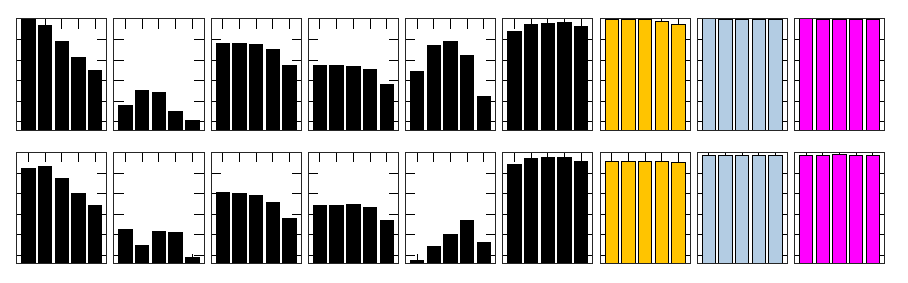
\includegraphics{./figures/parts/02/chapters/04/sections/05/pose_improvement_percent}}%
    \gplfronttext
  \end{picture}%
\endgroup

  \vspace{0.75cm}
  \caption{\small Τα ποσοστά επίτευξης του στόχου (\ref{objective:02_04}) ανά
           αλγόριθμο υπό δοκιμή, τυπική απόκλιση διαταραχών που επιδρούν στις
           πραγματικές μετρήσεις $\sigma_R$, και τυπική απόκλιση διαταραχών των
           συντεταγμένων του χάρτη $\sigma_{\bm{M}}$. Το διάγραμμα αυτό
           απαντάει στην ερώτηση: ``Από τον συνολικό αριθμό εκτιμήσεων στάσης
           που εισήχθησαν σε κάθε μέθοδο, ποιό είναι το ποσοστό των
           εκτιμήσεων των οποίων το σφάλμα μειώθηκε ως αποτέλεσμα της εφαμογής
           της κάθε μίας;". Κάθε ράβδος αντιστοιχεί σε $\approx
           4.5$$\cdot$$10\texttt{e}$$+$$5$ πειράματα ευθυγράμμισης, για όλες
           τις μεθόδους εκτός των NDT-PSO και TEASER, οι οποίες δοκιμάσθηκαν
           στο ένα δέκατο αυτής της τιμής λόγω του υπέρογκου χρόνου εκτέλεσής
           τους.  Σ.τ.Σ.: Αυτό το διάγραμμα είναι το σημαντικότερο του
           κεφαλαίου και ίσως το σημαντικότερο της διατριβής: οι σχεδιασθεντες
           σε αυτήν μέθοδοι \textit{διατηρούν την ευρωστία τους κατά μήκος
           των διαταραχών που επιδρούν στις μετρήσεις του φυσικού αισθητήρα
           δεδομένου ενός επιπέδου διαφθοράς χαρτη \underline{και} εκτελούνται
           σε πραγματικό χρόνο}, σε αντίθεση με όλους τους υπό δοκιμή
           αλγορίθμους της βιβλιογραφίας}
  \label{fig:02_04_05:01}
\end{figure}

\begin{figure}[!h]\vspace{3cm}%
  \definecolor{c1}{rgb}{0 0.4470 0.7410}
\definecolor{c2}{rgb}{0.8500 0.3250 0.0980}
\definecolor{c3}{rgb}{0.9290 0.6940 0.1250}
\definecolor{c4}{rgb}{0.4940 0.1840 0.5560}
\definecolor{c5}{rgb}{0.4660 0.6740 0.1880}
\definecolor{c6}{rgb}{0.3010 0.7450 0.9330}
\definecolor{c7}{RGB}{251,180,185}
\definecolor{c8}{RGB}{247,104,161}
\definecolor{c9}{RGB}{255,0,255}
\definecolor{g}{RGB}{44,162,95}
\definecolor{r}{RGB}{227,0,0}

% GNUPLOT: LaTeX picture with Postscript
\begingroup
  \makeatletter
  \providecommand\color[2][]{%
    \GenericError{(gnuplot) \space\space\space\@spaces}{%
      Package color not loaded in conjunction with
      terminal option `colourtext'%
    }{See the gnuplot documentation for explanation.%
    }{Either use 'blacktext' in gnuplot or load the package
      color.sty in LaTeX.}%
    \renewcommand\color[2][]{}%
  }%
  \providecommand\includegraphics[2][]{%
    \GenericError{(gnuplot) \space\space\space\@spaces}{%
      Package graphicx or graphics not loaded%
    }{See the gnuplot documentation for explanation.%
    }{The gnuplot epslatex terminal needs graphicx.sty or graphics.sty.}%
    \renewcommand\includegraphics[2][]{}%
  }%
  \providecommand\rotatebox[2]{#2}%
  \@ifundefined{ifGPcolor}{%
    \newif\ifGPcolor
    \GPcolorfalse
  }{}%
  \@ifundefined{ifGPblacktext}{%
    \newif\ifGPblacktext
    \GPblacktexttrue
  }{}%
  % define a \g@addto@macro without @ in the name:
  \let\gplgaddtomacro\g@addto@macro
  % define empty templates for all commands taking text:
  \gdef\gplfronttext{}%
  \gdef\gplfronttext{}%
  \makeatother
  \ifGPblacktext
    % no textcolor at all
    \def\colorrgb#1{}%
    \def\colorgray#1{}%
  \else
    % gray or color?
    \ifGPcolor
      \def\colorrgb#1{\color[rgb]{#1}}%
      \def\colorgray#1{\color[gray]{#1}}%
      \expandafter\def\csname LTw\endcsname{\color{white}}%
      \expandafter\def\csname LTb\endcsname{\color{black}}%
      \expandafter\def\csname LTa\endcsname{\color{black}}%
      \expandafter\def\csname LT0\endcsname{\color[rgb]{1,0,0}}%
      \expandafter\def\csname LT1\endcsname{\color[rgb]{0,1,0}}%
      \expandafter\def\csname LT2\endcsname{\color[rgb]{0,0,1}}%
      \expandafter\def\csname LT3\endcsname{\color[rgb]{1,0,1}}%
      \expandafter\def\csname LT4\endcsname{\color[rgb]{0,1,1}}%
      \expandafter\def\csname LT5\endcsname{\color[rgb]{1,1,0}}%
      \expandafter\def\csname LT6\endcsname{\color[rgb]{0,0,0}}%
      \expandafter\def\csname LT7\endcsname{\color[rgb]{1,0.3,0}}%
      \expandafter\def\csname LT8\endcsname{\color[rgb]{0.5,0.5,0.5}}%
    \else
      % gray
      \def\colorrgb#1{\color{black}}%
      \def\colorgray#1{\color[gray]{#1}}%
      \expandafter\def\csname LTw\endcsname{\color{white}}%
      \expandafter\def\csname LTb\endcsname{\color{black}}%
      \expandafter\def\csname LTa\endcsname{\color{black}}%
      \expandafter\def\csname LT0\endcsname{\color{black}}%
      \expandafter\def\csname LT1\endcsname{\color{black}}%
      \expandafter\def\csname LT2\endcsname{\color{black}}%
      \expandafter\def\csname LT3\endcsname{\color{black}}%
      \expandafter\def\csname LT4\endcsname{\color{black}}%
      \expandafter\def\csname LT5\endcsname{\color{black}}%
      \expandafter\def\csname LT6\endcsname{\color{black}}%
      \expandafter\def\csname LT7\endcsname{\color{black}}%
      \expandafter\def\csname LT8\endcsname{\color{black}}%
    \fi
  \fi
    \setlength{\unitlength}{0.0500bp}%
    \ifx\gptboxheight\undefined%
      \newlength{\gptboxheight}%
      \newlength{\gptboxwidth}%
      \newsavebox{\gptboxtext}%
    \fi%
    \setlength{\fboxrule}{0.5pt}%
    \setlength{\fboxsep}{1pt}%
    \hspace{1.75cm}
\begin{picture}(8000.00,7000.00)%
    \gplgaddtomacro\gplfronttext{%
      \colorrgb{0.15,0.15,0.15}%
      \put(-52,5715){\makebox(0,0)[r]{\strut{}\small $1.0$$\cdot$$10^5$}}%
      \colorrgb{0.15,0.15,0.15}%
      \put(-52,6221){\makebox(0,0)[r]{\strut{}\small $1.5$$\cdot$$10^5$}}%
      \colorrgb{0.15,0.15,0.15}%
      \put(-52,6727){\makebox(0,0)[r]{\strut{}\small $2.0$$\cdot$$10^5$}}%
      \colorrgb{0.15,0.15,0.15}%
      \put(303,5394){\makebox(0,0){\strut{}}}%
      \colorrgb{0.15,0.15,0.15}%
      \put(1194,5394){\makebox(0,0){\strut{}}}%
      \colorrgb{0.15,0.15,0.15}%
      \put(2085,5394){\makebox(0,0){\strut{}}}%
      \colorrgb{0.15,0.15,0.15}%
      \put(2843,5394){\makebox(0,0){\strut{}}}%
      \put(1639,7149){\makebox(0,0){\strut{}{\color{g}{$\|e(\bm{p}, \hat{\bm{p}}^\prime)\|_2 < \|e(\bm{p}, \hat{\bm{p}})\|_2$}}}}%
      \put(6359,7149){\makebox(0,0){\strut{}{\color{r}{$\|e(\bm{p}, \hat{\bm{p}}^\prime)\|_2 \geq \|e(\bm{p}, \hat{\bm{p}})\|_2$}}}}%

      \put(-400,7800){\makebox(0,0){\strut{}{\color{c1}{\rule[0.6mm]{0.5cm}{0.5mm}}}\small PLICP}}
      \put(600,7800){\makebox(0,0){\strut{}{\color{c2}{\rule[0.6mm]{0.5cm}{0.5mm}}}\small NDT}}
      \put(1600,7800){\makebox(0,0){\strut{}{\color{c3}{\rule[0.6mm]{0.5cm}{0.5mm}}}\small FastGICP}}
      \put(3000,7800){\makebox(0,0){\strut{}{\color{c4}{\rule[0.6mm]{0.5cm}{0.5mm}}}\small FastVGICP}}
      \put(4400,7800){\makebox(0,0){\strut{}{\color{c5}{\rule[0.6mm]{0.5cm}{0.5mm}}}\small NDT-PSO}}
      \put(5700,7800){\makebox(0,0){\strut{}{\color{c6}{\rule[0.6mm]{0.5cm}{0.5mm}}}\small TEASER}}
      \put(6600,7800){\makebox(0,0){\strut{}{\color{c7}{\rule[0.6mm]{0.5cm}{0.5mm}}}\small x1}}
      \put(7200,7800){\makebox(0,0){\strut{}{\color{c8}{\rule[0.6mm]{0.5cm}{0.5mm}}}\small uf}}
      \put(7800,7800){\makebox(0,0){\strut{}{\color{c9}{\rule[0.6mm]{0.5cm}{0.5mm}}}\small fm}}


      \put(-1542,6271){\rotatebox{90}{\makebox(0,0){\strut{}\small $\sigma_R = 0.01$ m}}}%
      \put(-1542,4885){\rotatebox{90}{\makebox(0,0){\strut{}\small $\sigma_R = 0.03$ m}}}%
      \put(-1542,3499){\rotatebox{90}{\makebox(0,0){\strut{}\small $\sigma_R = 0.05$ m}}}%
      \put(-1542,2113){\rotatebox{90}{\makebox(0,0){\strut{}\small $\sigma_R = 0.10$ m}}}%
      \put(-1542,727){\rotatebox{90}{\makebox(0,0) {\strut{}\small $\sigma_R = 0.20$ m}}}%

      \put(-942,3499){\rotatebox{90}{\makebox(0,0){\strut{}$-\sum \|e(\bm{p},\hat{\bm{p}}_i^\prime)\|_2-\|e(\bm{p},\hat{\bm{p}}_i)\|_2$}}}%
      \put(3999,3499){\rotatebox{90}{\makebox(0,0){\strut{}$+\sum \|e(\bm{p},\hat{\bm{p}}_i^\prime)\|_2-\|e(\bm{p},\hat{\bm{p}}_i)\|_2$}}}%
      \put(3999,8200){\makebox(0,0){\strut{}$\sigma_{\bm{M}} = 0.0$ m}}
    }%
    \gplgaddtomacro\gplfronttext{%
      \colorrgb{0.00,0.00,0.00}%
    }%
    \gplgaddtomacro\gplfronttext{%
      \colorrgb{0.15,0.15,0.15}%
      \put(-52,4329){\makebox(0,0)[r]{\strut{}\small $1.0$$\cdot$$10^5$}}%
      \colorrgb{0.15,0.15,0.15}%
      \put(-52,4835){\makebox(0,0)[r]{\strut{}\small $1.5$$\cdot$$10^5$}}%
      \colorrgb{0.15,0.15,0.15}%
      \put(-52,5341){\makebox(0,0)[r]{\strut{}\small $2.0$$\cdot$$10^5$}}%
      \colorrgb{0.15,0.15,0.15}%
      \put(303,4008){\makebox(0,0){\strut{}}}%
      \colorrgb{0.15,0.15,0.15}%
      \put(1194,4008){\makebox(0,0){\strut{}}}%
      \colorrgb{0.15,0.15,0.15}%
      \put(2085,4008){\makebox(0,0){\strut{}}}%
      \colorrgb{0.15,0.15,0.15}%
      \put(2843,4008){\makebox(0,0){\strut{}}}%
    }%
    \gplgaddtomacro\gplfronttext{%
    }%
    \gplgaddtomacro\gplfronttext{%
      \colorrgb{0.15,0.15,0.15}%
      \put(-52,2943){\makebox(0,0)[r]{\strut{}\small $1.0$$\cdot$$10^5$}}%
      \colorrgb{0.15,0.15,0.15}%
      \put(-52,3449){\makebox(0,0)[r]{\strut{}\small $1.5$$\cdot$$10^5$}}%
      \colorrgb{0.15,0.15,0.15}%
      \put(-52,3955){\makebox(0,0)[r]{\strut{}\small $2.0$$\cdot$$10^5$}}%
      \colorrgb{0.15,0.15,0.15}%
      \put(303,2622){\makebox(0,0){\strut{}}}%
      \colorrgb{0.15,0.15,0.15}%
      \put(1194,2622){\makebox(0,0){\strut{}}}%
      \colorrgb{0.15,0.15,0.15}%
      \put(2085,2622){\makebox(0,0){\strut{}}}%
      \colorrgb{0.15,0.15,0.15}%
      \put(2843,2622){\makebox(0,0){\strut{}}}%
    }%
    \gplgaddtomacro\gplfronttext{%
      \colorrgb{0.15,0.15,0.15}%
    }%
    \gplgaddtomacro\gplfronttext{%
      \colorrgb{0.15,0.15,0.15}%
      \put(-52,1557){\makebox(0,0)[r]{\strut{}\small $1.0$$\cdot$$10^5$}}%
      \colorrgb{0.15,0.15,0.15}%
      \put(-52,2063){\makebox(0,0)[r]{\strut{}\small $1.5$$\cdot$$10^5$}}%
      \colorrgb{0.15,0.15,0.15}%
      \put(-52,2569){\makebox(0,0)[r]{\strut{}\small $2.0$$\cdot$$10^5$}}%
      \colorrgb{0.15,0.15,0.15}%
      \put(303,1236){\makebox(0,0){\strut{}}}%
      \colorrgb{0.15,0.15,0.15}%
      \put(1194,1236){\makebox(0,0){\strut{}}}%
      \colorrgb{0.15,0.15,0.15}%
      \put(2085,1236){\makebox(0,0){\strut{}}}%
      \colorrgb{0.15,0.15,0.15}%
      \put(2843,1236){\makebox(0,0){\strut{}}}%
    }%
    \gplgaddtomacro\gplfronttext{%
    }%
    \gplgaddtomacro\gplfronttext{%
      \colorrgb{0.15,0.15,0.15}%
      \put(-52,171){\makebox(0,0)[r]{\strut{}\small $1.0$$\cdot$$10^5$}}%
      \colorrgb{0.15,0.15,0.15}%
      \put(-52,677){\makebox(0,0)[r]{\strut{}\small $1.5$$\cdot$$10^5$}}%
      \colorrgb{0.15,0.15,0.15}%
      \put(-52,1183){\makebox(0,0)[r]{\strut{}\small $2.0$$\cdot$$10^5$}}%
      \colorrgb{0.15,0.15,0.15}%
      \put(303,-150){\makebox(0,0){\strut{}\small $3.4$$\cdot$$10^5$}}%
      \colorrgb{0.15,0.15,0.15}%
      \put(1194,-150){\makebox(0,0){\strut{}\small $3.8$$\cdot$$10^5$}}%
      \colorrgb{0.15,0.15,0.15}%
      \put(2085,-150){\makebox(0,0){\strut{}\small $4.2$$\cdot$$10^5$}}%
      \colorrgb{0.15,0.15,0.15}%
      \put(2843,-150){\makebox(0,0){\strut{}\small $E$$\cdot$$|D|$}}%
    }%
    \gplgaddtomacro\gplfronttext{%
      \colorrgb{0.15,0.15,0.15}%
      \put(1639,-480){\makebox(0,0){\strut{}$|\{\hat{\bm{p}}_{i}^\prime\}| : \|e(\bm{p}, \hat{\bm{p}}_i^\prime)\|_2 < \|e(\bm{p}, \hat{\bm{p}}_i)\|_2$}}%
    }%
    \gplgaddtomacro\gplfronttext{%
      \colorrgb{0.15,0.15,0.15}%
      \put(4668,5614){\makebox(0,0)[r]{\strut{}\small $10^{-1}$}}%
      \colorrgb{0.15,0.15,0.15}%
      \put(4668,5947){\makebox(0,0)[r]{\strut{}\small $10^{+1}$}}%
      \colorrgb{0.15,0.15,0.15}%
      \put(4668,6280){\makebox(0,0)[r]{\strut{}\small $10^{+3}$}}%
      \colorrgb{0.15,0.15,0.15}%
      \put(4668,6612){\makebox(0,0)[r]{\strut{}\small $10^{+5}$}}%
      \colorrgb{0.15,0.15,0.15}%
      \put(4850,5394){\makebox(0,0){\strut{}}}%
      \colorrgb{0.15,0.15,0.15}%
      \put(5365,5394){\makebox(0,0){\strut{}}}%
      \colorrgb{0.15,0.15,0.15}%
      \put(5881,5394){\makebox(0,0){\strut{}}}%
      \colorrgb{0.15,0.15,0.15}%
      \put(6396,5394){\makebox(0,0){\strut{}}}%
      \colorrgb{0.15,0.15,0.15}%
      \put(6912,5394){\makebox(0,0){\strut{}}}%
      \colorrgb{0.15,0.15,0.15}%
      \put(7427,5394){\makebox(0,0){\strut{}}}%
      \colorrgb{0.15,0.15,0.15}%
      \put(7766,5394){\makebox(0,0){\strut{}}}%
    }%
    \gplgaddtomacro\gplfronttext{%
      \colorrgb{0.00,0.00,0.00}%
    }%
    \gplgaddtomacro\gplfronttext{%
      \colorrgb{0.15,0.15,0.15}%
      \put(4668,4228){\makebox(0,0)[r]{\strut{}\small $10^{-1}$}}%
      \colorrgb{0.15,0.15,0.15}%
      \put(4668,4561){\makebox(0,0)[r]{\strut{}\small $10^{+1}$}}%
      \colorrgb{0.15,0.15,0.15}%
      \put(4668,4894){\makebox(0,0)[r]{\strut{}\small $10^{+3}$}}%
      \colorrgb{0.15,0.15,0.15}%
      \put(4668,5226){\makebox(0,0)[r]{\strut{}\small $10^{+5}$}}%
      \colorrgb{0.15,0.15,0.15}%
      \put(4850,4008){\makebox(0,0){\strut{}}}%
      \colorrgb{0.15,0.15,0.15}%
      \put(5365,4008){\makebox(0,0){\strut{}}}%
      \colorrgb{0.15,0.15,0.15}%
      \put(5881,4008){\makebox(0,0){\strut{}}}%
      \colorrgb{0.15,0.15,0.15}%
      \put(6396,4008){\makebox(0,0){\strut{}}}%
      \colorrgb{0.15,0.15,0.15}%
      \put(6912,4008){\makebox(0,0){\strut{}}}%
      \colorrgb{0.15,0.15,0.15}%
      \put(7427,4008){\makebox(0,0){\strut{}}}%
      \colorrgb{0.15,0.15,0.15}%
      \put(7766,4008){\makebox(0,0){\strut{}}}%
    }%
    \gplgaddtomacro\gplfronttext{%
    }%
    \gplgaddtomacro\gplfronttext{%
      \colorrgb{0.15,0.15,0.15}%
      \put(4668,2842){\makebox(0,0)[r]{\strut{}\small $10^{-1}$}}%
      \colorrgb{0.15,0.15,0.15}%
      \put(4668,3175){\makebox(0,0)[r]{\strut{}\small $10^{+1}$}}%
      \colorrgb{0.15,0.15,0.15}%
      \put(4668,3508){\makebox(0,0)[r]{\strut{}\small $10^{+3}$}}%
      \colorrgb{0.15,0.15,0.15}%
      \put(4668,3840){\makebox(0,0)[r]{\strut{}\small $10^{+5}$}}%
      \colorrgb{0.15,0.15,0.15}%
      \put(4850,2622){\makebox(0,0){\strut{}}}%
      \colorrgb{0.15,0.15,0.15}%
      \put(5365,2622){\makebox(0,0){\strut{}}}%
      \colorrgb{0.15,0.15,0.15}%
      \put(5881,2622){\makebox(0,0){\strut{}}}%
      \colorrgb{0.15,0.15,0.15}%
      \put(6396,2622){\makebox(0,0){\strut{}}}%
      \colorrgb{0.15,0.15,0.15}%
      \put(6912,2622){\makebox(0,0){\strut{}}}%
      \colorrgb{0.15,0.15,0.15}%
      \put(7427,2622){\makebox(0,0){\strut{}}}%
      \colorrgb{0.15,0.15,0.15}%
      \put(7766,2622){\makebox(0,0){\strut{}}}%
    }%
    \gplgaddtomacro\gplfronttext{%
      \colorrgb{0.15,0.15,0.15}%
    }%
    \gplgaddtomacro\gplfronttext{%
      \colorrgb{0.15,0.15,0.15}%
      \put(4668,1456){\makebox(0,0)[r]{\strut{}\small $10^{-1}$}}%
      \colorrgb{0.15,0.15,0.15}%
      \put(4668,1789){\makebox(0,0)[r]{\strut{}\small $10^{+1}$}}%
      \colorrgb{0.15,0.15,0.15}%
      \put(4668,2122){\makebox(0,0)[r]{\strut{}\small $10^{+3}$}}%
      \colorrgb{0.15,0.15,0.15}%
      \put(4668,2454){\makebox(0,0)[r]{\strut{}\small $10^{+5}$}}%
      \colorrgb{0.15,0.15,0.15}%
      \put(4850,1236){\makebox(0,0){\strut{}}}%
      \colorrgb{0.15,0.15,0.15}%
      \put(5365,1236){\makebox(0,0){\strut{}}}%
      \colorrgb{0.15,0.15,0.15}%
      \put(5881,1236){\makebox(0,0){\strut{}}}%
      \colorrgb{0.15,0.15,0.15}%
      \put(6396,1236){\makebox(0,0){\strut{}}}%
      \colorrgb{0.15,0.15,0.15}%
      \put(6912,1236){\makebox(0,0){\strut{}}}%
      \colorrgb{0.15,0.15,0.15}%
      \put(7427,1236){\makebox(0,0){\strut{}}}%
      \colorrgb{0.15,0.15,0.15}%
      \put(7766,1236){\makebox(0,0){\strut{}}}%
    }%
    \gplgaddtomacro\gplfronttext{%
    }%
    \gplgaddtomacro\gplfronttext{%
      \colorrgb{0.15,0.15,0.15}%
      \put(4668,70){\makebox(0,0)[r]{\strut{}\small $10^{-1}$}}%
      \colorrgb{0.15,0.15,0.15}%
      \put(4668,403){\makebox(0,0)[r]{\strut{}\small $10^{+1}$}}%
      \colorrgb{0.15,0.15,0.15}%
      \put(4668,736){\makebox(0,0)[r]{\strut{}\small $10^{+3}$}}%
      \colorrgb{0.15,0.15,0.15}%
      \put(4668,1068){\makebox(0,0)[r]{\strut{}\small $10^{+5}$}}%
      \colorrgb{0.15,0.15,0.15}%
      \put(4850,-150){\makebox(0,0){\strut{}\small $10^0$}}%
      \colorrgb{0.15,0.15,0.15}%
      \put(5365,-150){\makebox(0,0){\strut{}\small $10^1$}}%
      \colorrgb{0.15,0.15,0.15}%
      \put(5881,-150){\makebox(0,0){\strut{}\small $10^2$}}%
      \colorrgb{0.15,0.15,0.15}%
      \put(6396,-150){\makebox(0,0){\strut{}\small $10^3$}}%
      \colorrgb{0.15,0.15,0.15}%
      \put(6912,-150){\makebox(0,0){\strut{}\small $10^4$}}%
      \colorrgb{0.15,0.15,0.15}%
      \put(7427,-150){\makebox(0,0){\strut{}}}%
      \colorrgb{0.15,0.15,0.15}%
      \put(7766,-150){\makebox(0,0){\strut{}\small $E$$\cdot$$|D|$}}%
    }%
    \gplgaddtomacro\gplfronttext{%
      \colorrgb{0.15,0.15,0.15}%
      \put(6359,-480){\makebox(0,0){\strut{}$|\{\hat{\bm{p}}_{i}^\prime\}| : \|e(\bm{p}, \hat{\bm{p}}_i^\prime)\|_2 \geq \|e(\bm{p}, \hat{\bm{p}}_i)\|_2$}}%
    }%
    \put(0,0){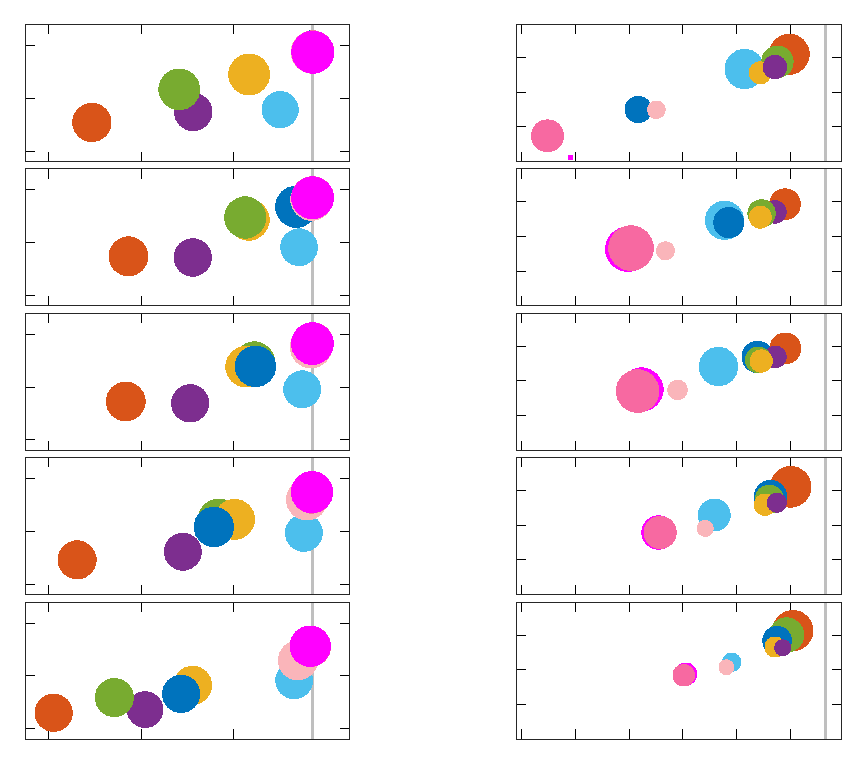
\includegraphics{./figures/parts/02/chapters/04/sections/05/pose_improvement_circles_sm0}}%
    \gplfronttext
  \end{picture}%
\endgroup

  \vspace{1cm}
  \caption{\small Η συνολική μείωση (αριστερά, στον κάθετο άξονα) και αύξηση
           (δεξιά) του σφάλματος εκτίμησης στάσης συναρτήσει του αριθμού των
           δειγμάτων των οποίων το μέτρο σφάλματος εκτίμησης στάσης μειώθηκε
           (αριστερά, στον οριζόντιο άξονα) και αυξήθηκε (δεξιά), για
           $\sigma_{\bm{M}} = 0.0$ m. Η ακτίνα των κύκλων είναι ανάλογη της
           μέσης μείωσης (αύξησης) ανά στάση για την οποία το σφάλμα μειώθηκε
           (αυξήθηκε) ως αποτέλεσμα της εφαρμογής κάθε μεθόδου.  Αυτό το
           διάγραμμα απαντάει στις εξής ερωτήσεις: (α) ``Από τον συνολικό
           αριθμό εκτιμήσεων στάσης που εισήχθησαν σε κάθε μέθοδο, πόσων το
           σφάλμα κατάφερε η κάθε μέθοδος να μειώσει, και σε πόσες απέτυχε;",
           (β) ``Από τον συνολικό αριθμό εκτιμήσεων στάσης που εισήχθησαν σε
           κάθε μέθοδο, πόσο είναι το συνολικό σφάλμα που κατάφερε να μειώσει η
           καθεμία;", (γ) ``Από τον συνολικό αριθμό εκτιμήσεων στάσης που
           εισήχθησαν σε κάθε μέθοδο, πόσο είναι το συνολικό σφάλμα που επέφερε
           η καθεμία όταν δεν κατάφερε να μειώσει το σφάλμα της αρχικής
           εκτίμησης;", και (δ) ``Ποιό είναι το μέσο σφάλμα κατά το οποίο
           μειώθηκε (αυξήθηκε) μία αρχική εκτίμηση για αυτές των οποίων το
           σφάλμα μειώθηκε (αυξήθηκε);"}
  \label{fig:02_04_05:01_circles_sm0}
\end{figure}

\begin{figure}[!h]\vspace{3cm}%
  \definecolor{c1}{rgb}{0 0.4470 0.7410}
\definecolor{c2}{rgb}{0.8500 0.3250 0.0980}
\definecolor{c3}{rgb}{0.9290 0.6940 0.1250}
\definecolor{c4}{rgb}{0.4940 0.1840 0.5560}
\definecolor{c5}{rgb}{0.4660 0.6740 0.1880}
\definecolor{c6}{rgb}{0.3010 0.7450 0.9330}
\definecolor{c7}{RGB}{251,180,185}
\definecolor{c8}{RGB}{247,104,161}
\definecolor{c9}{RGB}{255,0,255}
\definecolor{g}{RGB}{44,162,95}
\definecolor{r}{RGB}{227,0,0}

% GNUPLOT: LaTeX picture with Postscript
\begingroup
  \makeatletter
  \providecommand\color[2][]{%
    \GenericError{(gnuplot) \space\space\space\@spaces}{%
      Package color not loaded in conjunction with
      terminal option `colourtext'%
    }{See the gnuplot documentation for explanation.%
    }{Either use 'blacktext' in gnuplot or load the package
      color.sty in LaTeX.}%
    \renewcommand\color[2][]{}%
  }%
  \providecommand\includegraphics[2][]{%
    \GenericError{(gnuplot) \space\space\space\@spaces}{%
      Package graphicx or graphics not loaded%
    }{See the gnuplot documentation for explanation.%
    }{The gnuplot epslatex terminal needs graphicx.sty or graphics.sty.}%
    \renewcommand\includegraphics[2][]{}%
  }%
  \providecommand\rotatebox[2]{#2}%
  \@ifundefined{ifGPcolor}{%
    \newif\ifGPcolor
    \GPcolorfalse
  }{}%
  \@ifundefined{ifGPblacktext}{%
    \newif\ifGPblacktext
    \GPblacktexttrue
  }{}%
  % define a \g@addto@macro without @ in the name:
  \let\gplgaddtomacro\g@addto@macro
  % define empty templates for all commands taking text:
  \gdef\gplfronttext{}%
  \gdef\gplfronttext{}%
  \makeatother
  \ifGPblacktext
    % no textcolor at all
    \def\colorrgb#1{}%
    \def\colorgray#1{}%
  \else
    % gray or color?
    \ifGPcolor
      \def\colorrgb#1{\color[rgb]{#1}}%
      \def\colorgray#1{\color[gray]{#1}}%
      \expandafter\def\csname LTw\endcsname{\color{white}}%
      \expandafter\def\csname LTb\endcsname{\color{black}}%
      \expandafter\def\csname LTa\endcsname{\color{black}}%
      \expandafter\def\csname LT0\endcsname{\color[rgb]{1,0,0}}%
      \expandafter\def\csname LT1\endcsname{\color[rgb]{0,1,0}}%
      \expandafter\def\csname LT2\endcsname{\color[rgb]{0,0,1}}%
      \expandafter\def\csname LT3\endcsname{\color[rgb]{1,0,1}}%
      \expandafter\def\csname LT4\endcsname{\color[rgb]{0,1,1}}%
      \expandafter\def\csname LT5\endcsname{\color[rgb]{1,1,0}}%
      \expandafter\def\csname LT6\endcsname{\color[rgb]{0,0,0}}%
      \expandafter\def\csname LT7\endcsname{\color[rgb]{1,0.3,0}}%
      \expandafter\def\csname LT8\endcsname{\color[rgb]{0.5,0.5,0.5}}%
    \else
      % gray
      \def\colorrgb#1{\color{black}}%
      \def\colorgray#1{\color[gray]{#1}}%
      \expandafter\def\csname LTw\endcsname{\color{white}}%
      \expandafter\def\csname LTb\endcsname{\color{black}}%
      \expandafter\def\csname LTa\endcsname{\color{black}}%
      \expandafter\def\csname LT0\endcsname{\color{black}}%
      \expandafter\def\csname LT1\endcsname{\color{black}}%
      \expandafter\def\csname LT2\endcsname{\color{black}}%
      \expandafter\def\csname LT3\endcsname{\color{black}}%
      \expandafter\def\csname LT4\endcsname{\color{black}}%
      \expandafter\def\csname LT5\endcsname{\color{black}}%
      \expandafter\def\csname LT6\endcsname{\color{black}}%
      \expandafter\def\csname LT7\endcsname{\color{black}}%
      \expandafter\def\csname LT8\endcsname{\color{black}}%
    \fi
  \fi
    \setlength{\unitlength}{0.0500bp}%
    \ifx\gptboxheight\undefined%
      \newlength{\gptboxheight}%
      \newlength{\gptboxwidth}%
      \newsavebox{\gptboxtext}%
    \fi%
    \setlength{\fboxrule}{0.5pt}%
    \setlength{\fboxsep}{1pt}%

    \hspace{1.75cm}
\begin{picture}(8000.00,7000.00)%
    \gplgaddtomacro\gplfronttext{%
      \colorrgb{0.15,0.15,0.15}%
      \put(-52,5734){\makebox(0,0)[r]{\strut{}\small $1.0$$\cdot$$10^5$}}%
      \colorrgb{0.15,0.15,0.15}%
      \put(-52,6331){\makebox(0,0)[r]{\strut{}\small $1.5$$\cdot$$10^5$}}%
      \colorrgb{0.15,0.15,0.15}%
      \put(-52,6929){\makebox(0,0)[r]{\strut{}\small $2.0$$\cdot$$10^5$}}%
      \colorrgb{0.15,0.15,0.15}%
      \put(80,5394){\makebox(0,0){\strut{}}}%
      \colorrgb{0.15,0.15,0.15}%
      \put(1328,5394){\makebox(0,0){\strut{}}}%
      \colorrgb{0.15,0.15,0.15}%
      \put(2159,5394){\makebox(0,0){\strut{}}}%
      \colorrgb{0.15,0.15,0.15}%
      \put(2867,5394){\makebox(0,0){\strut{}}}%
    }%
    \gplgaddtomacro\gplfronttext{%
      \colorrgb{0.00,0.00,0.00}%
      \put(1639,7149){\makebox(0,0){\strut{}{\color{g}{$\|e(\bm{p}, \hat{\bm{p}}^\prime)\|_2 < \|e(\bm{p}, \hat{\bm{p}})\|_2$}}}}%
      \put(6359,7149){\makebox(0,0){\strut{}{\color{r}{$\|e(\bm{p}, \hat{\bm{p}}^\prime)\|_2 \geq \|e(\bm{p}, \hat{\bm{p}})\|_2$}}}}%

      \put(-400,7800){\makebox(0,0){\strut{}{\color{c1}{\rule[0.6mm]{0.5cm}{0.5mm}}}\small PLICP}}
      \put(600,7800){\makebox(0,0){\strut{}{\color{c2}{\rule[0.6mm]{0.5cm}{0.5mm}}}\small NDT}}
      \put(1600,7800){\makebox(0,0){\strut{}{\color{c3}{\rule[0.6mm]{0.5cm}{0.5mm}}}\small FastGICP}}
      \put(3000,7800){\makebox(0,0){\strut{}{\color{c4}{\rule[0.6mm]{0.5cm}{0.5mm}}}\small FastVGICP}}
      \put(4400,7800){\makebox(0,0){\strut{}{\color{c5}{\rule[0.6mm]{0.5cm}{0.5mm}}}\small NDT-PSO}}
      \put(5700,7800){\makebox(0,0){\strut{}{\color{c6}{\rule[0.6mm]{0.5cm}{0.5mm}}}\small TEASER}}
      \put(6600,7800){\makebox(0,0){\strut{}{\color{c7}{\rule[0.6mm]{0.5cm}{0.5mm}}}\small x1}}
      \put(7200,7800){\makebox(0,0){\strut{}{\color{c8}{\rule[0.6mm]{0.5cm}{0.5mm}}}\small uf}}
      \put(7800,7800){\makebox(0,0){\strut{}{\color{c9}{\rule[0.6mm]{0.5cm}{0.5mm}}}\small fm}}


      \put(-1542,6271){\rotatebox{90}{\makebox(0,0){\strut{}\small $\sigma_R = 0.01$ m}}}%
      \put(-1542,4885){\rotatebox{90}{\makebox(0,0){\strut{}\small $\sigma_R = 0.03$ m}}}%
      \put(-1542,3499){\rotatebox{90}{\makebox(0,0){\strut{}\small $\sigma_R = 0.05$ m}}}%
      \put(-1542,2113){\rotatebox{90}{\makebox(0,0){\strut{}\small $\sigma_R = 0.10$ m}}}%
      \put(-1542,727){\rotatebox{90}{\makebox(0,0) {\strut{}\small $\sigma_R = 0.20$ m}}}%

      \put(-942,3499){\rotatebox{90}{\makebox(0,0){\strut{}$-\sum \|e(\bm{p},\hat{\bm{p}}_i^\prime)\|_2-\|e(\bm{p},\hat{\bm{p}}_i)\|_2$}}}%
      \put(3999,3499){\rotatebox{90}{\makebox(0,0){\strut{}$+\sum \|e(\bm{p},\hat{\bm{p}}_i^\prime)\|_2-\|e(\bm{p},\hat{\bm{p}}_i)\|_2$}}}%
      \put(3999,8200){\makebox(0,0){\strut{}$\sigma_{\bm{M}} = 0.05$ m}}
    }%
    \gplgaddtomacro\gplfronttext{%
      \colorrgb{0.15,0.15,0.15}%
      \put(-52,4348){\makebox(0,0)[r]{\strut{}\small $1.0$$\cdot$$10^5$}}%
      \colorrgb{0.15,0.15,0.15}%
      \put(-52,4945){\makebox(0,0)[r]{\strut{}\small $1.5$$\cdot$$10^5$}}%
      \colorrgb{0.15,0.15,0.15}%
      \put(-52,5543){\makebox(0,0)[r]{\strut{}\small $2.0$$\cdot$$10^5$}}%
      \colorrgb{0.15,0.15,0.15}%
      \put(80,4008){\makebox(0,0){\strut{}}}%
      \colorrgb{0.15,0.15,0.15}%
      \put(1328,4008){\makebox(0,0){\strut{}}}%
      \colorrgb{0.15,0.15,0.15}%
      \put(2159,4008){\makebox(0,0){\strut{}}}%
      \colorrgb{0.15,0.15,0.15}%
      \put(2867,4008){\makebox(0,0){\strut{}}}%
    }%
    \gplgaddtomacro\gplfronttext{%
    }%
    \gplgaddtomacro\gplfronttext{%
      \colorrgb{0.15,0.15,0.15}%
      \put(-52,2962){\makebox(0,0)[r]{\strut{}\small $1.0$$\cdot$$10^5$}}%
      \colorrgb{0.15,0.15,0.15}%
      \put(-52,3559){\makebox(0,0)[r]{\strut{}\small $1.5$$\cdot$$10^5$}}%
      \colorrgb{0.15,0.15,0.15}%
      \put(-52,4157){\makebox(0,0)[r]{\strut{}\small $2.0$$\cdot$$10^5$}}%
      \colorrgb{0.15,0.15,0.15}%
      \put(80,2622){\makebox(0,0){\strut{}}}%
      \colorrgb{0.15,0.15,0.15}%
      \put(1328,2622){\makebox(0,0){\strut{}}}%
      \colorrgb{0.15,0.15,0.15}%
      \put(2159,2622){\makebox(0,0){\strut{}}}%
      \colorrgb{0.15,0.15,0.15}%
      \put(2867,2622){\makebox(0,0){\strut{}}}%
    }%
    \gplgaddtomacro\gplfronttext{%
      \colorrgb{0.15,0.15,0.15}%
    }%
    \gplgaddtomacro\gplfronttext{%
      \colorrgb{0.15,0.15,0.15}%
      \put(-52,1576){\makebox(0,0)[r]{\strut{}\small $1.0$$\cdot$$10^5$}}%
      \colorrgb{0.15,0.15,0.15}%
      \put(-52,2173){\makebox(0,0)[r]{\strut{}\small $1.5$$\cdot$$10^5$}}%
      \colorrgb{0.15,0.15,0.15}%
      \put(-52,2771){\makebox(0,0)[r]{\strut{}\small $2.0$$\cdot$$10^5$}}%
      \colorrgb{0.15,0.15,0.15}%
      \put(80,1236){\makebox(0,0){\strut{}}}%
      \colorrgb{0.15,0.15,0.15}%
      \put(1328,1236){\makebox(0,0){\strut{}}}%
      \colorrgb{0.15,0.15,0.15}%
      \put(2159,1236){\makebox(0,0){\strut{}}}%
      \colorrgb{0.15,0.15,0.15}%
      \put(2867,1236){\makebox(0,0){\strut{}}}%
    }%
    \gplgaddtomacro\gplfronttext{%
    }%
    \gplgaddtomacro\gplfronttext{%
      \colorrgb{0.15,0.15,0.15}%
      \put(-52,190){\makebox(0,0)[r]{\strut{}\small $1.0$$\cdot$$10^5$}}%
      \colorrgb{0.15,0.15,0.15}%
      \put(-52,787){\makebox(0,0)[r]{\strut{}\small $1.5$$\cdot$$10^5$}}%
      \colorrgb{0.15,0.15,0.15}%
      \put(-52,1385){\makebox(0,0)[r]{\strut{}\small $2.0$$\cdot$$10^5$}}%
      \colorrgb{0.15,0.15,0.15}%
      \put(80,-150){\makebox(0,0){\strut{}\small $3.2$$\cdot$$10^5$}}%
      \colorrgb{0.15,0.15,0.15}%
      \put(1328,-150){\makebox(0,0){\strut{}\small $3.8$$\cdot$$10^5$}}%
      \colorrgb{0.15,0.15,0.15}%
      \put(2159,-150){\makebox(0,0){\strut{}\small $4.2$$\cdot$$10^5$}}%
      \colorrgb{0.15,0.15,0.15}%
      \put(2867,-150){\makebox(0,0){\strut{}\small $E$$\cdot$$|D|$}}%
    }%
    \gplgaddtomacro\gplfronttext{%
      \colorrgb{0.15,0.15,0.15}%
      \put(1639,-480){\makebox(0,0){\strut{}$|\{\hat{\bm{p}}_{i}^\prime\}| : \|e(\bm{p}, \hat{\bm{p}}_i^\prime)\|_2 < \|e(\bm{p}, \hat{\bm{p}}_i)\|_2$}}%
    }%
    \gplgaddtomacro\gplfronttext{%
      \colorrgb{0.15,0.15,0.15}%
      \put(4668,5614){\makebox(0,0)[r]{\strut{}\small $10^{+2}$}}%
      \colorrgb{0.15,0.15,0.15}%
      \put(4668,6174){\makebox(0,0)[r]{\strut{}\small $10^{+4}$}}%
      \colorrgb{0.15,0.15,0.15}%
      \put(4668,6733){\makebox(0,0)[r]{\strut{}\small $10^{+6}$}}%
      \colorrgb{0.15,0.15,0.15}%
      \put(4800,5394){\makebox(0,0){\strut{}}}%
      \colorrgb{0.15,0.15,0.15}%
      \put(5974,5394){\makebox(0,0){\strut{}}}%
      \colorrgb{0.15,0.15,0.15}%
      \put(7148,5394){\makebox(0,0){\strut{}}}%
      \colorrgb{0.15,0.15,0.15}%
      \put(7919,5394){\makebox(0,0){\strut{}}}%
    }%
    \gplgaddtomacro\gplfronttext{%
      \colorrgb{0.00,0.00,0.00}%
    }%
    \gplgaddtomacro\gplfronttext{%
      \colorrgb{0.15,0.15,0.15}%
      \put(4668,4228){\makebox(0,0)[r]{\strut{}\small $10^{+2}$}}%
      \colorrgb{0.15,0.15,0.15}%
      \put(4668,4788){\makebox(0,0)[r]{\strut{}\small $10^{+4}$}}%
      \colorrgb{0.15,0.15,0.15}%
      \put(4668,5347){\makebox(0,0)[r]{\strut{}\small $10^{+6}$}}%
      \colorrgb{0.15,0.15,0.15}%
      \put(4800,4008){\makebox(0,0){\strut{}}}%
      \colorrgb{0.15,0.15,0.15}%
      \put(5974,4008){\makebox(0,0){\strut{}}}%
      \colorrgb{0.15,0.15,0.15}%
      \put(7148,4008){\makebox(0,0){\strut{}}}%
      \colorrgb{0.15,0.15,0.15}%
      \put(7919,4008){\makebox(0,0){\strut{}}}%
    }%
    \gplgaddtomacro\gplfronttext{%
    }%
    \gplgaddtomacro\gplfronttext{%
      \colorrgb{0.15,0.15,0.15}%
      \put(4668,2842){\makebox(0,0)[r]{\strut{}\small $10^{+2}$}}%
      \colorrgb{0.15,0.15,0.15}%
      \put(4668,3402){\makebox(0,0)[r]{\strut{}\small $10^{+4}$}}%
      \colorrgb{0.15,0.15,0.15}%
      \put(4668,3961){\makebox(0,0)[r]{\strut{}\small $10^{+6}$}}%
      \colorrgb{0.15,0.15,0.15}%
      \put(4800,2622){\makebox(0,0){\strut{}}}%
      \colorrgb{0.15,0.15,0.15}%
      \put(5974,2622){\makebox(0,0){\strut{}}}%
      \colorrgb{0.15,0.15,0.15}%
      \put(7148,2622){\makebox(0,0){\strut{}}}%
      \colorrgb{0.15,0.15,0.15}%
      \put(7919,2622){\makebox(0,0){\strut{}}}%
    }%
    \gplgaddtomacro\gplfronttext{%
      \colorrgb{0.15,0.15,0.15}%
    }%
    \gplgaddtomacro\gplfronttext{%
      \colorrgb{0.15,0.15,0.15}%
      \put(4668,1456){\makebox(0,0)[r]{\strut{}\small $10^{+2}$}}%
      \colorrgb{0.15,0.15,0.15}%
      \put(4668,2016){\makebox(0,0)[r]{\strut{}\small $10^{+4}$}}%
      \colorrgb{0.15,0.15,0.15}%
      \put(4668,2575){\makebox(0,0)[r]{\strut{}\small $10^{+6}$}}%
      \colorrgb{0.15,0.15,0.15}%
      \put(4800,1236){\makebox(0,0){\strut{}}}%
      \colorrgb{0.15,0.15,0.15}%
      \put(5974,1236){\makebox(0,0){\strut{}}}%
      \colorrgb{0.15,0.15,0.15}%
      \put(7148,1236){\makebox(0,0){\strut{}}}%
      \colorrgb{0.15,0.15,0.15}%
      \put(7919,1236){\makebox(0,0){\strut{}}}%
    }%
    \gplgaddtomacro\gplfronttext{%
    }%
    \gplgaddtomacro\gplfronttext{%
      \colorrgb{0.15,0.15,0.15}%
      \put(4668,70){\makebox(0,0)[r]{\strut{}\small $10^{+2}$}}%
      \colorrgb{0.15,0.15,0.15}%
      \put(4668,630){\makebox(0,0)[r]{\strut{}\small $10^{+4}$}}%
      \colorrgb{0.15,0.15,0.15}%
      \put(4668,1189){\makebox(0,0)[r]{\strut{}\small $10^{+6}$}}%
      \colorrgb{0.15,0.15,0.15}%
      \put(4800,-150){\makebox(0,0){\strut{}\small $10^3$}}%
      \colorrgb{0.15,0.15,0.15}%
      \put(5974,-150){\makebox(0,0){\strut{}\small $10^4$}}%
      \colorrgb{0.15,0.15,0.15}%
      \put(7148,-150){\makebox(0,0){\strut{}\small $10^5$}}%
      \colorrgb{0.15,0.15,0.15}%
      \put(7919,-150){\makebox(0,0){\strut{}\small $E$$\cdot$$|D|$}}%
    }%
    \gplgaddtomacro\gplfronttext{%
      \colorrgb{0.15,0.15,0.15}%
      \put(6359,-480){\makebox(0,0){\strut{}$|\{\hat{\bm{p}}_{i}^\prime\}| : \|e(\bm{p}, \hat{\bm{p}}_i^\prime)\|_2 \geq \|e(\bm{p}, \hat{\bm{p}}_i)\|_2$}}%
    }%
    \put(0,0){\includegraphics{./figures/parts/02/chapters/04/sections/05//pose_improvement_circles_sm5}}%
    \gplfronttext
  \end{picture}%
\endgroup

  \vspace{1cm}
  \caption{\small Η συνολική μείωση (αριστερά, στον κάθετο άξονα) και αύξηση
           (δεξιά) του σφάλματος εκτίμησης στάσης συναρτήσει του αριθμού των
           δειγμάτων των οποίων το μέτρο σφάλματος εκτίμησης στάσης μειώθηκε
           (αριστερά, στον οριζόντιο άξονα) και αυξήθηκε (δεξιά), για
           $\sigma_{\bm{M}} = 0.05$ m. Η ακτίνα των κύκλων είναι ανάλογη της
           μέσης μείωσης (αύξησης) ανά στάση για την οποία το σφάλμα μειώθηκε
           (αυξήθηκε) ως αποτέλεσμα της εφαρμογής κάθε μεθόδου. Αυτό το
           διάγραμμα απαντάει στις εξής ερωτήσεις: (α) ``Από τον συνολικό
           αριθμό εκτιμήσεων στάσης που εισήχθησαν σε κάθε μέθοδο, πόσων το
           σφάλμα κατάφερε η κάθε μέθοδος να μειώσει, και σε πόσες απέτυχε;",
           (β) ``Από τον συνολικό αριθμό εκτιμήσεων στάσης που εισήχθησαν σε
           κάθε μέθοδο, πόσο είναι το συνολικό σφάλμα που κατάφερε να μειώσει η
           καθεμία;", (γ) ``Από τον συνολικό αριθμό εκτιμήσεων στάσης που
           εισήχθησαν σε κάθε μέθοδο, πόσο είναι το συνολικό σφάλμα που επέφερε
           η καθεμία όταν δεν κατάφερε να μειώσει το σφάλμα της αρχικής
           εκτίμησης;", και (δ) ``Ποιό είναι το μέσο σφάλμα κατά το οποίο
           μειώθηκε (αυξήθηκε) μία αρχική εκτίμηση για αυτές των οποίων το
           σφάλμα μειώθηκε (αυξήθηκε);"}
  \label{fig:02_04_05:01_circles_sm5}
\end{figure}

Στο σχήμα \ref{fig:02_04_05:02} απεικονίζονται οι κατανομες των καθαρών χρόνων
εκτέλεσης του κάθε αλγορίθμου, δηλαδή ο ολικός χρόνος εκτέλεσης των άνευ του
χρόνου εκτέλεσης υπολογισμού εικονικών σαρώσεων. Στην άνω σειρά του σχήματος
\ref{fig:02_04_05:03} απεικονιζεται η κατανομή του αριθμού των εικονικών
σαρώσεων που συνέλαβαν οι τρεις όψεις του FSMSM, και στη μεσαία ο ολικος χρόνος
εκτέλεσής τους για τη διαμόρφωση που περιγράφηκε στην ενότητα
\ref{subsection:02_04_05:01}. Στην τελευταία σειρά απεικονίζονται οι χρόνοι
εκτέλεσης των τριων μεθοδων για την ίδια διαμόρφωση εάν όμως η αναπαράσταση του
χάρτη γινόταν μέσω χάρτη πλέγματος. Η διαφορά ανάμεσα στους δύο χρόνους
εκτέλεσης έγκειται στο γεγονός ότι ο υπολογισμός εικονικών σαρώσεων σε χάρτες
πλέγματος γίνεται σε πολύ μικρότερο χρόνο ($\approx 30\%$) σε σχέση με την
υλοποίηση που ακολουθήσαμε \cite{Walsh2018}. Με βάση τα στοιχεία του σχήματος
\ref{fig:02_04_05:04}, ο λόγος για τις αυξημένες τιμές χρόνου εκτέλεσης της
μεθόδου \texttt{x1} σε σχέση με αυτές των \texttt{uf} και \texttt{fm} οφείλεται
στον αυξημένο αριθμό επανεκκινήσεων της πρώτης.

\begin{figure}[!h]
  \definecolor{c1}{rgb}{0 0.4470 0.7410}
\definecolor{c2}{rgb}{0.8500 0.3250 0.0980}
\definecolor{c3}{rgb}{0.9290 0.6940 0.1250}
\definecolor{c4}{rgb}{0.4940 0.1840 0.5560}
\definecolor{c5}{rgb}{0.4660 0.6740 0.1880}
\definecolor{c6}{rgb}{0.3010 0.7450 0.9330}
\definecolor{c7}{RGB}{251,180,185}
\definecolor{c8}{RGB}{247,104,161}
\definecolor{c9}{RGB}{255,0,255}

% GNUPLOT: LaTeX picture with Postscript
\begingroup
  \makeatletter
  \providecommand\color[2][]{%
    \GenericError{(gnuplot) \space\space\space\@spaces}{%
      Package color not loaded in conjunction with
      terminal option `colourtext'%
    }{See the gnuplot documentation for explanation.%
    }{Either use 'blacktext' in gnuplot or load the package
      color.sty in LaTeX.}%
    \renewcommand\color[2][]{}%
  }%
  \providecommand\includegraphics[2][]{%
    \GenericError{(gnuplot) \space\space\space\@spaces}{%
      Package graphicx or graphics not loaded%
    }{See the gnuplot documentation for explanation.%
    }{The gnuplot epslatex terminal needs graphicx.sty or graphics.sty.}%
    \renewcommand\includegraphics[2][]{}%
  }%
  \providecommand\rotatebox[2]{#2}%
  \@ifundefined{ifGPcolor}{%
    \newif\ifGPcolor
    \GPcolorfalse
  }{}%
  \@ifundefined{ifGPblacktext}{%
    \newif\ifGPblacktext
    \GPblacktexttrue
  }{}%
  % define a \g@addto@macro without @ in the name:
  \let\gplgaddtomacro\g@addto@macro
  % define empty templates for all commands taking text:
  \gdef\gplbacktext{}%
  \gdef\gplfronttext{}%
  \makeatother
  \ifGPblacktext
    % no textcolor at all
    \def\colorrgb#1{}%
    \def\colorgray#1{}%
  \else
    % gray or color?
    \ifGPcolor
      \def\colorrgb#1{\color[rgb]{#1}}%
      \def\colorgray#1{\color[gray]{#1}}%
      \expandafter\def\csname LTw\endcsname{\color{white}}%
      \expandafter\def\csname LTb\endcsname{\color{black}}%
      \expandafter\def\csname LTa\endcsname{\color{black}}%
      \expandafter\def\csname LT0\endcsname{\color[rgb]{1,0,0}}%
      \expandafter\def\csname LT1\endcsname{\color[rgb]{0,1,0}}%
      \expandafter\def\csname LT2\endcsname{\color[rgb]{0,0,1}}%
      \expandafter\def\csname LT3\endcsname{\color[rgb]{1,0,1}}%
      \expandafter\def\csname LT4\endcsname{\color[rgb]{0,1,1}}%
      \expandafter\def\csname LT5\endcsname{\color[rgb]{1,1,0}}%
      \expandafter\def\csname LT6\endcsname{\color[rgb]{0,0,0}}%
      \expandafter\def\csname LT7\endcsname{\color[rgb]{1,0.3,0}}%
      \expandafter\def\csname LT8\endcsname{\color[rgb]{0.5,0.5,0.5}}%
    \else
      % gray
      \def\colorrgb#1{\color{black}}%
      \def\colorgray#1{\color[gray]{#1}}%
      \expandafter\def\csname LTw\endcsname{\color{white}}%
      \expandafter\def\csname LTb\endcsname{\color{black}}%
      \expandafter\def\csname LTa\endcsname{\color{black}}%
      \expandafter\def\csname LT0\endcsname{\color{black}}%
      \expandafter\def\csname LT1\endcsname{\color{black}}%
      \expandafter\def\csname LT2\endcsname{\color{black}}%
      \expandafter\def\csname LT3\endcsname{\color{black}}%
      \expandafter\def\csname LT4\endcsname{\color{black}}%
      \expandafter\def\csname LT5\endcsname{\color{black}}%
      \expandafter\def\csname LT6\endcsname{\color{black}}%
      \expandafter\def\csname LT7\endcsname{\color{black}}%
      \expandafter\def\csname LT8\endcsname{\color{black}}%
    \fi
  \fi
    \setlength{\unitlength}{0.0500bp}%
    \ifx\gptboxheight\undefined%
      \newlength{\gptboxheight}%
      \newlength{\gptboxwidth}%
      \newsavebox{\gptboxtext}%
    \fi%
    \setlength{\fboxrule}{0.5pt}%
    \setlength{\fboxsep}{1pt}%
\begin{picture}(9600.00,4000.00)%
    \gplgaddtomacro\gplbacktext{%
      \colorrgb{0.15,0.15,0.15}%
      \put(828,2656){\makebox(0,0)[r]{\strut{}$10^{-2}$}}%
      \colorrgb{0.15,0.15,0.15}%
      \put(828,3051){\makebox(0,0)[r]{\strut{}$10^{-1}$}}%
      \colorrgb{0.15,0.15,0.15}%
      \put(828,3445){\makebox(0,0)[r]{\strut{}$10^{0}$}}%
      \colorrgb{0.15,0.15,0.15}%
      \put(828,3840){\makebox(0,0)[r]{\strut{}$10^{1}$}}%
      \colorrgb{0.15,0.15,0.15}%
      \put(1728,2160){\makebox(0,0){\strut{}}}%
      \colorrgb{0.15,0.15,0.15}%
      \put(3264,2160){\makebox(0,0){\strut{}}}%
      \colorrgb{0.15,0.15,0.15}%
      \put(4800,2160){\makebox(0,0){\strut{}}}%
      \colorrgb{0.15,0.15,0.15}%
      \put(6335,2160){\makebox(0,0){\strut{}}}%
      \colorrgb{0.15,0.15,0.15}%
      \put(7871,2160){\makebox(0,0){\strut{}}}%
    }%
    \gplgaddtomacro\gplfronttext{%
      \colorrgb{0.00,0.00,0.00}%
      \put(4799,4179){\makebox(0,0){\strut{}$\sigma_{\bm{M}} = 0.0$ m}}%
      \put(600,4700){\makebox(0,0){\strut{}{\color{c1}{\rule[0.6mm]{0.5cm}{0.5mm}}}\small PLICP}}
      \put(1600,4700){\makebox(0,0){\strut{}{\color{c2}{\rule[0.6mm]{0.5cm}{0.5mm}}}\small NDT}}
      \put(2600,4700){\makebox(0,0){\strut{}{\color{c3}{\rule[0.6mm]{0.5cm}{0.5mm}}}\small FastGICP}}
      \put(4000,4700){\makebox(0,0){\strut{}{\color{c4}{\rule[0.6mm]{0.5cm}{0.5mm}}}\small FastVGICP}}
      \put(5400,4700){\makebox(0,0){\strut{}{\color{c5}{\rule[0.6mm]{0.5cm}{0.5mm}}}\small NDT-PSO}}
      \put(6700,4700){\makebox(0,0){\strut{}{\color{c6}{\rule[0.6mm]{0.5cm}{0.5mm}}}\small TEASER}}
      \put(7600,4700){\makebox(0,0){\strut{}{\color{c7}{\rule[0.6mm]{0.5cm}{0.5mm}}}\small x1}}
      \put(8200,4700){\makebox(0,0){\strut{}{\color{c8}{\rule[0.6mm]{0.5cm}{0.5mm}}}\small uf}}
      \put(8800,4700){\makebox(0,0){\strut{}{\color{c9}{\rule[0.6mm]{0.5cm}{0.5mm}}}\small fm}}
      \put(4799,5200){\makebox(0,0){\strut{}Κατανομή καθαρού χρόνου εκτέλεσης [sec]}}%
    }%
    \gplgaddtomacro\gplbacktext{%
      \colorrgb{0.15,0.15,0.15}%
      \put(828,316){\makebox(0,0)[r]{\strut{}$10^{-2}$}}%
      \colorrgb{0.15,0.15,0.15}%
      \put(828,711){\makebox(0,0)[r]{\strut{}$10^{-1}$}}%
      \colorrgb{0.15,0.15,0.15}%
      \put(828,1105){\makebox(0,0)[r]{\strut{}$10^{0}$}}%
      \colorrgb{0.15,0.15,0.15}%
      \put(828,1500){\makebox(0,0)[r]{\strut{}$10^{1}$}}%
      \colorrgb{0.15,0.15,0.15}%
      \put(1728,-180){\makebox(0,0){\strut{}}}%
      \colorrgb{0.15,0.15,0.15}%
      \put(3264,-180){\makebox(0,0){\strut{}}}%
      \colorrgb{0.15,0.15,0.15}%
      \put(4800,-180){\makebox(0,0){\strut{}}}%
      \colorrgb{0.15,0.15,0.15}%
      \put(6335,-180){\makebox(0,0){\strut{}}}%
      \colorrgb{0.15,0.15,0.15}%
      \put(7871,-180){\makebox(0,0){\strut{}}}%
    }%
    \gplgaddtomacro\gplfronttext{%
      \colorrgb{0.15,0.15,0.15}%
      \put(4799,-510){\makebox(0,0){\strut{}Τυπική απόκλιση διαταραχών $\sigma_R$ [m]}}%
      \colorrgb{0.00,0.00,0.00}%
      \put(4799,1839){\makebox(0,0){\strut{}$\sigma_{\bm{M}} = 0.05$ m}}%
    }%
    \gplbacktext
    \put(0,0){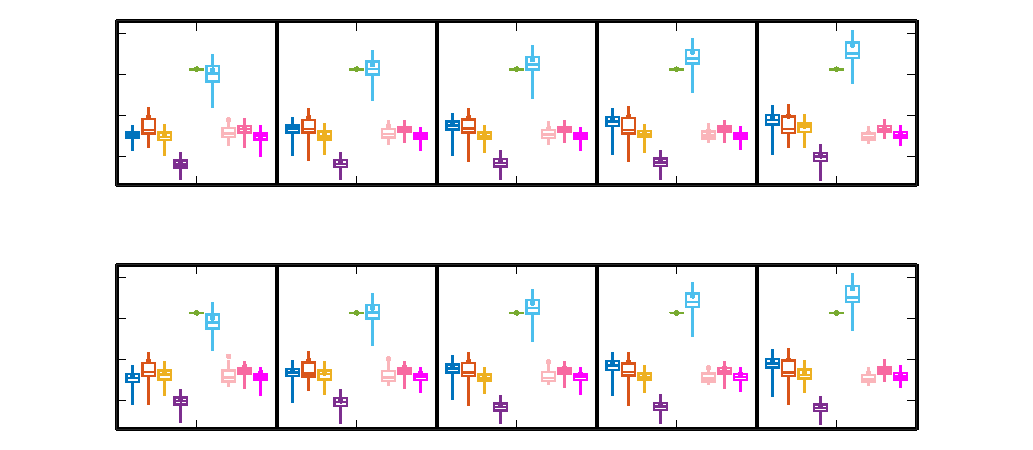
\includegraphics{./figures/parts/02/chapters/04/sections/05/boxplots_execution_times}}%
    \gplfronttext
  \end{picture}%
\endgroup

  \vspace{1cm}
  \caption{\small Οι κατανομές των χρόνων εκτέλεσης όλων των αλγορίθμων χωρίς να
           συνυπολογίζεται ο χρόνος υπολογισμού σαρώσεων χάρτη. Για τους
           \texttt{x1}, \texttt{uf}, και \texttt{fm}, ο ολικός χρόνος εκτέλεσης
           με βαση τη διαμόρφωση της ενότητας \ref{subsection:02_04_05:01}
           απεικονίζεται στο σχήμα \ref{fig:02_04_05:03}. Παρατηρήστε πως η
           εκτέλεση των μεθόδων NDT-PSO και TEASER σε τέσσερα επεξεργαστικά
           νήματα έχει ως αποτέλεσμα χρόνους εκτέλεσης άνω του ενός
           δευτερολέπτου, δηλαδή η εκτέλεσή τους γίνεται σε μη πραγματικό
           χρόνο}
  \label{fig:02_04_05:02}
\end{figure}

\begin{figure}[!h]
  \definecolor{c7}{RGB}{251,180,185}
\definecolor{c8}{RGB}{247,104,161}
\definecolor{c9}{RGB}{255,0,255}

% GNUPLOT: LaTeX picture with Postscript
\begingroup
  \makeatletter
  \providecommand\color[2][]{%
    \GenericError{(gnuplot) \space\space\space\@spaces}{%
      Package color not loaded in conjunction with
      terminal option `colourtext'%
    }{See the gnuplot documentation for explanation.%
    }{Either use 'blacktext' in gnuplot or load the package
      color.sty in LaTeX.}%
    \renewcommand\color[2][]{}%
  }%
  \providecommand\includegraphics[2][]{%
    \GenericError{(gnuplot) \space\space\space\@spaces}{%
      Package graphicx or graphics not loaded%
    }{See the gnuplot documentation for explanation.%
    }{The gnuplot epslatex terminal needs graphicx.sty or graphics.sty.}%
    \renewcommand\includegraphics[2][]{}%
  }%
  \providecommand\rotatebox[2]{#2}%
  \@ifundefined{ifGPcolor}{%
    \newif\ifGPcolor
    \GPcolorfalse
  }{}%
  \@ifundefined{ifGPblacktext}{%
    \newif\ifGPblacktext
    \GPblacktexttrue
  }{}%
  % define a \g@addto@macro without @ in the name:
  \let\gplgaddtomacro\g@addto@macro
  % define empty templates for all commands taking text:
  \gdef\gplfronttext{}%
  \gdef\gplfronttext{}%
  \makeatother
  \ifGPblacktext
    % no textcolor at all
    \def\colorrgb#1{}%
    \def\colorgray#1{}%
  \else
    % gray or color?
    \ifGPcolor
      \def\colorrgb#1{\color[rgb]{#1}}%
      \def\colorgray#1{\color[gray]{#1}}%
      \expandafter\def\csname LTw\endcsname{\color{white}}%
      \expandafter\def\csname LTb\endcsname{\color{black}}%
      \expandafter\def\csname LTa\endcsname{\color{black}}%
      \expandafter\def\csname LT0\endcsname{\color[rgb]{1,0,0}}%
      \expandafter\def\csname LT1\endcsname{\color[rgb]{0,1,0}}%
      \expandafter\def\csname LT2\endcsname{\color[rgb]{0,0,1}}%
      \expandafter\def\csname LT3\endcsname{\color[rgb]{1,0,1}}%
      \expandafter\def\csname LT4\endcsname{\color[rgb]{0,1,1}}%
      \expandafter\def\csname LT5\endcsname{\color[rgb]{1,1,0}}%
      \expandafter\def\csname LT6\endcsname{\color[rgb]{0,0,0}}%
      \expandafter\def\csname LT7\endcsname{\color[rgb]{1,0.3,0}}%
      \expandafter\def\csname LT8\endcsname{\color[rgb]{0.5,0.5,0.5}}%
    \else
      % gray
      \def\colorrgb#1{\color{black}}%
      \def\colorgray#1{\color[gray]{#1}}%
      \expandafter\def\csname LTw\endcsname{\color{white}}%
      \expandafter\def\csname LTb\endcsname{\color{black}}%
      \expandafter\def\csname LTa\endcsname{\color{black}}%
      \expandafter\def\csname LT0\endcsname{\color{black}}%
      \expandafter\def\csname LT1\endcsname{\color{black}}%
      \expandafter\def\csname LT2\endcsname{\color{black}}%
      \expandafter\def\csname LT3\endcsname{\color{black}}%
      \expandafter\def\csname LT4\endcsname{\color{black}}%
      \expandafter\def\csname LT5\endcsname{\color{black}}%
      \expandafter\def\csname LT6\endcsname{\color{black}}%
      \expandafter\def\csname LT7\endcsname{\color{black}}%
      \expandafter\def\csname LT8\endcsname{\color{black}}%
    \fi
  \fi
    \setlength{\unitlength}{0.0500bp}%
    \ifx\gptboxheight\undefined%
      \newlength{\gptboxheight}%
      \newlength{\gptboxwidth}%
      \newsavebox{\gptboxtext}%
    \fi%
    \setlength{\fboxrule}{0.5pt}%
    \setlength{\fboxsep}{1pt}%
\begin{picture}(8000.00,6000.00)%
    \gplgaddtomacro\gplfronttext{%
      \colorrgb{0.15,0.15,0.15}%
      \put(-52,4522){\makebox(0,0)[r]{\strut{}\small $100$}}%
      \colorrgb{0.15,0.15,0.15}%
      \put(-52,4940){\makebox(0,0)[r]{\strut{}\small $200$}}%
      \colorrgb{0.15,0.15,0.15}%
      \put(-52,5184){\makebox(0,0)[r]{\strut{}\small $300$}}%
      \colorrgb{0.15,0.15,0.15}%
      \put(-52,5358){\makebox(0,0)[r]{\strut{}\small $400$}}%
      \colorrgb{0.15,0.15,0.15}%
      \put(-52,5775){\makebox(0,0)[r]{\strut{}\small $800$}}%
      \colorrgb{0.15,0.15,0.15}%
      \put(-52,5910){\makebox(0,0)[r]{\strut{}\small $1000$}}%
      \colorrgb{0.15,0.15,0.15}%
      \put(468,4239){\makebox(0,0){\strut{}}}%
      \colorrgb{0.15,0.15,0.15}%
      \put(1244,4239){\makebox(0,0){\strut{}}}%
      \colorrgb{0.15,0.15,0.15}%
      \put(2020,4239){\makebox(0,0){\strut{}}}%
      \colorrgb{0.15,0.15,0.15}%
      \put(2795,4239){\makebox(0,0){\strut{}}}%
      \colorrgb{0.15,0.15,0.15}%
      \put(3571,4239){\makebox(0,0){\strut{}}}%
    }%
    \gplgaddtomacro\gplfronttext{%
      \colorrgb{0.00,0.00,0.00}%
      \put(3999,6159){\makebox(0,0){\strut{}Κατανομή αριθμού σαρώσεων χάρτη}}%
      \put(2019,6559){\makebox(0,0){\strut{}$\sigma_{\bm{M}} = 0.0$ m}}%
      \put(6019,6559){\makebox(0,0){\strut{}$\sigma_{\bm{M}} = 0.05$ m}}%
      \put(2999,6959){\makebox(0,0){\strut{}{\color{c7}{\rule[0.6mm]{0.5cm}{0.5mm}}}\small x1}}
      \put(3999,6959){\makebox(0,0){\strut{}{\color{c8}{\rule[0.6mm]{0.5cm}{0.5mm}}}\small uf}}
      \put(4999,6959){\makebox(0,0){\strut{}{\color{c9}{\rule[0.6mm]{0.5cm}{0.5mm}}}\small fm}}
    }%
    \gplgaddtomacro\gplfronttext{%
      \colorrgb{0.15,0.15,0.15}%
      \put(3908,4522){\makebox(0,0)[r]{\strut{}}}%
      \colorrgb{0.15,0.15,0.15}%
      \put(3908,4940){\makebox(0,0)[r]{\strut{}}}%
      \colorrgb{0.15,0.15,0.15}%
      \put(3908,5184){\makebox(0,0)[r]{\strut{}}}%
      \colorrgb{0.15,0.15,0.15}%
      \put(3908,5358){\makebox(0,0)[r]{\strut{}}}%
      \colorrgb{0.15,0.15,0.15}%
      \put(3908,5775){\makebox(0,0)[r]{\strut{}}}%
      \colorrgb{0.15,0.15,0.15}%
      \put(3908,5910){\makebox(0,0)[r]{\strut{}}}%
      \colorrgb{0.15,0.15,0.15}%
      \put(4428,4239){\makebox(0,0){\strut{}}}%
      \colorrgb{0.15,0.15,0.15}%
      \put(5204,4239){\makebox(0,0){\strut{}}}%
      \colorrgb{0.15,0.15,0.15}%
      \put(5980,4239){\makebox(0,0){\strut{}}}%
      \colorrgb{0.15,0.15,0.15}%
      \put(6755,4239){\makebox(0,0){\strut{}}}%
      \colorrgb{0.15,0.15,0.15}%
      \put(7531,4239){\makebox(0,0){\strut{}}}%
    }%
    \gplgaddtomacro\gplfronttext{%
    }%
    \gplgaddtomacro\gplfronttext{%
      \colorrgb{0.15,0.15,0.15}%
      \put(-52,2260){\makebox(0,0)[r]{\strut{}\small $0.0$}}%
      \colorrgb{0.15,0.15,0.15}%
      \put(-52,2683){\makebox(0,0)[r]{\strut{}\small $0.100$}}%
      \colorrgb{0.15,0.15,0.15}%
      \put(-52,3105){\makebox(0,0)[r]{\strut{}\small $0.200$}}%
      \colorrgb{0.15,0.15,0.15}%
      \put(-52,3528){\makebox(0,0)[r]{\strut{}\small $0.300$}}%
      \colorrgb{0.15,0.15,0.15}%
      \put(468,2040){\makebox(0,0){\strut{}}}%
      \colorrgb{0.15,0.15,0.15}%
      \put(1244,2040){\makebox(0,0){\strut{}}}%
      \colorrgb{0.15,0.15,0.15}%
      \put(2020,2040){\makebox(0,0){\strut{}}}%
      \colorrgb{0.15,0.15,0.15}%
      \put(2795,2040){\makebox(0,0){\strut{}}}%
      \colorrgb{0.15,0.15,0.15}%
      \put(3571,2040){\makebox(0,0){\strut{}}}%
    }%
    \gplgaddtomacro\gplfronttext{%
      \colorrgb{0.00,0.00,0.00}%
      \put(3999,3959){\makebox(0,0){\strut{}Κατανομή ολικού χρόνου εκτέλεσης [sec]}}%
    }%
    \gplgaddtomacro\gplfronttext{%
      \colorrgb{0.15,0.15,0.15}%
      \put(3908,2260){\makebox(0,0)[r]{\strut{}}}%
      \colorrgb{0.15,0.15,0.15}%
      \put(3908,2683){\makebox(0,0)[r]{\strut{}}}%
      \colorrgb{0.15,0.15,0.15}%
      \put(3908,3105){\makebox(0,0)[r]{\strut{}}}%
      \colorrgb{0.15,0.15,0.15}%
      \put(3908,3528){\makebox(0,0)[r]{\strut{}}}%
      \colorrgb{0.15,0.15,0.15}%
      \put(4428,2040){\makebox(0,0){\strut{}}}%
      \colorrgb{0.15,0.15,0.15}%
      \put(5204,2040){\makebox(0,0){\strut{}}}%
      \colorrgb{0.15,0.15,0.15}%
      \put(5980,2040){\makebox(0,0){\strut{}}}%
      \colorrgb{0.15,0.15,0.15}%
      \put(6755,2040){\makebox(0,0){\strut{}}}%
      \colorrgb{0.15,0.15,0.15}%
      \put(7531,2040){\makebox(0,0){\strut{}}}%
    }%
    \gplgaddtomacro\gplfronttext{%
    }%
    \gplgaddtomacro\gplfronttext{%
      \colorrgb{0.15,0.15,0.15}%
      \put(-52,60){\makebox(0,0)[r]{\strut{}\small $0.0$}}%
      \colorrgb{0.15,0.15,0.15}%
      \put(-52,483){\makebox(0,0)[r]{\strut{}\small $0.050$}}%
      \colorrgb{0.15,0.15,0.15}%
      \put(-52,905){\makebox(0,0)[r]{\strut{}\small $0.100$}}%
      \colorrgb{0.15,0.15,0.15}%
      \put(-52,1328){\makebox(0,0)[r]{\strut{}\small $0.150$}}%
      \colorrgb{0.15,0.15,0.15}%
      \put(468,-160){\makebox(0,0){\strut{}$0.01$}}%
      \colorrgb{0.15,0.15,0.15}%
      \put(1244,-160){\makebox(0,0){\strut{}$0.03$}}%
      \colorrgb{0.15,0.15,0.15}%
      \put(2020,-160){\makebox(0,0){\strut{}$0.05$}}%
      \colorrgb{0.15,0.15,0.15}%
      \put(2795,-160){\makebox(0,0){\strut{}$0.10$}}%
      \colorrgb{0.15,0.15,0.15}%
      \put(3571,-160){\makebox(0,0){\strut{}$0.20$}}%
    }%
    \gplgaddtomacro\gplfronttext{%
      \colorrgb{0.15,0.15,0.15}%
      \put(3999,-490){\makebox(0,0){\strut{}Τυπική απόκλιση διαταραχών $\sigma_R$ [m]}}%
      \colorrgb{0.00,0.00,0.00}%
      \put(3999,1759){\makebox(0,0){\strut{}Κατανομή ολικού χρόνου εκτέλεσης [sec] (Αναγωγή σε αναπαράσταση χάρτη μέσω πλέγματος)}}%
    }%
    \gplgaddtomacro\gplfronttext{%
      \colorrgb{0.15,0.15,0.15}%
      \put(3908,60){\makebox(0,0)[r]{\strut{}}}%
      \colorrgb{0.15,0.15,0.15}%
      \put(3908,483){\makebox(0,0)[r]{\strut{}}}%
      \colorrgb{0.15,0.15,0.15}%
      \put(3908,905){\makebox(0,0)[r]{\strut{}}}%
      \colorrgb{0.15,0.15,0.15}%
      \put(3908,1328){\makebox(0,0)[r]{\strut{}}}%
      \colorrgb{0.15,0.15,0.15}%
      \put(4428,-160){\makebox(0,0){\strut{}$0.01$}}%
      \colorrgb{0.15,0.15,0.15}%
      \put(5204,-160){\makebox(0,0){\strut{}$0.03$}}%
      \colorrgb{0.15,0.15,0.15}%
      \put(5980,-160){\makebox(0,0){\strut{}$0.05$}}%
      \colorrgb{0.15,0.15,0.15}%
      \put(6755,-160){\makebox(0,0){\strut{}$0.10$}}%
      \colorrgb{0.15,0.15,0.15}%
      \put(7531,-160){\makebox(0,0){\strut{}$0.20$}}%
    }%
    \gplgaddtomacro\gplfronttext{%
    }%
    \put(0,0){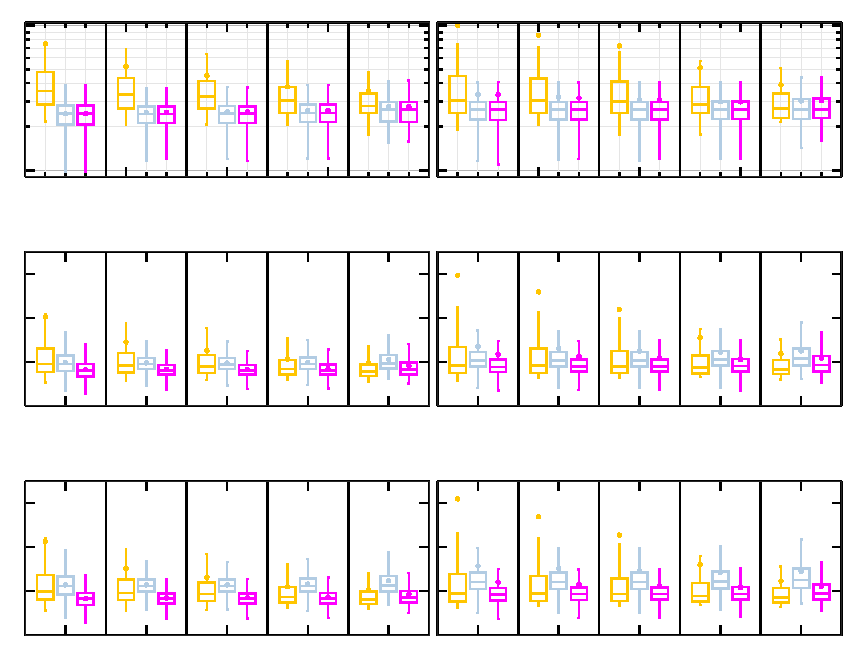
\includegraphics{./figures/parts/02/chapters/04/sections/05/boxplots_iterations}}%
    \gplfronttext
  \end{picture}%
\endgroup

  \vspace{1cm}
  \caption{\small Οι κατανομές του αριθμού των συλληφθέντων σαρώσεων χάρτη (άνω
           σειρά), των ολικών χρόνων εκτέλεσης με βάση τη διαμόρφωση της
           ενότητας \ref{subsection:02_04_05:01} (μεσαία), και του ανηγμένου
           χρόνου εκτέλεσης εάν ο χάρτης του κάθε περιβάλλοντος αναπαρίστατο
           μέσω πλέγματος}
  \label{fig:02_04_05:03}
\end{figure}

\begin{figure}[!h]\centering\vspace{1.5cm}
  \begin{subfigure}{\linewidth}
    \input{./figures/parts/02/chapters/04/sections/05/recoveries_sm0.tex}
  \end{subfigure}\\\vspace{2.2cm}%
  \begin{subfigure}{\linewidth}\hspace{1.0cm}
    % GNUPLOT: LaTeX picture with Postscript
\begingroup
  \makeatletter
  \providecommand\color[2][]{%
    \GenericError{(gnuplot) \space\space\space\@spaces}{%
      Package color not loaded in conjunction with
      terminal option `colourtext'%
    }{See the gnuplot documentation for explanation.%
    }{Either use 'blacktext' in gnuplot or load the package
      color.sty in LaTeX.}%
    \renewcommand\color[2][]{}%
  }%
  \providecommand\includegraphics[2][]{%
    \GenericError{(gnuplot) \space\space\space\@spaces}{%
      Package graphicx or graphics not loaded%
    }{See the gnuplot documentation for explanation.%
    }{The gnuplot epslatex terminal needs graphicx.sty or graphics.sty.}%
    \renewcommand\includegraphics[2][]{}%
  }%
  \providecommand\rotatebox[2]{#2}%
  \@ifundefined{ifGPcolor}{%
    \newif\ifGPcolor
    \GPcolorfalse
  }{}%
  \@ifundefined{ifGPblacktext}{%
    \newif\ifGPblacktext
    \GPblacktexttrue
  }{}%
  % define a \g@addto@macro without @ in the name:
  \let\gplgaddtomacro\g@addto@macro
  % define empty templates for all commands taking text:
  \gdef\gplfronttext{}%
  \gdef\gplfronttext{}%
  \makeatother
  \ifGPblacktext
    % no textcolor at all
    \def\colorrgb#1{}%
    \def\colorgray#1{}%
  \else
    % gray or color?
    \ifGPcolor
      \def\colorrgb#1{\color[rgb]{#1}}%
      \def\colorgray#1{\color[gray]{#1}}%
      \expandafter\def\csname LTw\endcsname{\color{white}}%
      \expandafter\def\csname LTb\endcsname{\color{black}}%
      \expandafter\def\csname LTa\endcsname{\color{black}}%
      \expandafter\def\csname LT0\endcsname{\color[rgb]{1,0,0}}%
      \expandafter\def\csname LT1\endcsname{\color[rgb]{0,1,0}}%
      \expandafter\def\csname LT2\endcsname{\color[rgb]{0,0,1}}%
      \expandafter\def\csname LT3\endcsname{\color[rgb]{1,0,1}}%
      \expandafter\def\csname LT4\endcsname{\color[rgb]{0,1,1}}%
      \expandafter\def\csname LT5\endcsname{\color[rgb]{1,1,0}}%
      \expandafter\def\csname LT6\endcsname{\color[rgb]{0,0,0}}%
      \expandafter\def\csname LT7\endcsname{\color[rgb]{1,0.3,0}}%
      \expandafter\def\csname LT8\endcsname{\color[rgb]{0.5,0.5,0.5}}%
    \else
      % gray
      \def\colorrgb#1{\color{black}}%
      \def\colorgray#1{\color[gray]{#1}}%
      \expandafter\def\csname LTw\endcsname{\color{white}}%
      \expandafter\def\csname LTb\endcsname{\color{black}}%
      \expandafter\def\csname LTa\endcsname{\color{black}}%
      \expandafter\def\csname LT0\endcsname{\color{black}}%
      \expandafter\def\csname LT1\endcsname{\color{black}}%
      \expandafter\def\csname LT2\endcsname{\color{black}}%
      \expandafter\def\csname LT3\endcsname{\color{black}}%
      \expandafter\def\csname LT4\endcsname{\color{black}}%
      \expandafter\def\csname LT5\endcsname{\color{black}}%
      \expandafter\def\csname LT6\endcsname{\color{black}}%
      \expandafter\def\csname LT7\endcsname{\color{black}}%
      \expandafter\def\csname LT8\endcsname{\color{black}}%
    \fi
  \fi
    \setlength{\unitlength}{0.0500bp}%
    \ifx\gptboxheight\undefined%
      \newlength{\gptboxheight}%
      \newlength{\gptboxwidth}%
      \newsavebox{\gptboxtext}%
    \fi%
    \setlength{\fboxrule}{0.5pt}%
    \setlength{\fboxsep}{1pt}%
\begin{picture}(8000.00,5000.00)%
    \gplgaddtomacro\gplfronttext{%
      \put(-548,4375){\rotatebox{90}{\makebox(0,0){\strut{}\texttt{x1}}}}%
      \put(-548,3125){\rotatebox{90}{\makebox(0,0){\strut{}\texttt{uf}}}}%
      \put(-548,1875){\rotatebox{90}{\makebox(0,0){\strut{}\texttt{fm}}}}%
      \put(-148,3125) {\rotatebox{90}{\makebox(0,0){\strut{}$\|\Delta \hat{\bm{l}}\|_2 \in [0, \sqrt{2} \cdot \overline{\delta}_{xy}]$}}}%
    }%
    \gplgaddtomacro\gplfronttext{%
      \colorrgb{0.15,0.15,0.15}%
      \put(3999,5450){\makebox(0,0){\strut{}$\sigma_{\bm{M}} = 0.05$ m}}%
      \put(816,5100) {\makebox(0,0){\strut{}$\sigma_R = 0.01$ m}}%
      \put(2432,5100){\makebox(0,0){\strut{}$\sigma_R = 0.03$ m}}%
      \put(4000,5100){\makebox(0,0){\strut{}$\sigma_R = 0.05$ m}}%
      \put(5568,5100){\makebox(0,0){\strut{}$\sigma_R = 0.10$ m}}%
      \put(7184,5100){\makebox(0,0){\strut{}$\sigma_R = 0.20$ m}}%
      \put(3999,1056){\makebox(0,0){\strut{}$\Delta\hat{\theta} \in [-\overline{\delta}_\theta, +\overline{\delta}_\theta]$}}
    }%
    \put(0,0){
\includegraphics{./figures/parts/02/chapters/04/sections/05/recoveries_sm5}}%
    \gplfronttext
  \end{picture}%
\endgroup

  \end{subfigure}%
  \vspace{-1cm}
\caption{\small Χάρτες θερμότητας του αριθμού των επανεκκινήσεων των
         μεθόδων \texttt{x1}, \texttt{uf}, και \texttt{fm} ανά επίπεδο
         διαταραχών των μετρήσεων της πραγματικής σάρωσης $\sigma_R$ και
         διαφθορας του χάρτη $\sigma_{\bm{M}}$. Ο οριζόντιος άξονας κάθε χάρτη
         θερμότητας αναφέρεται στο σφάλμα εκτίμησης προσανατολισμού
         $\Delta\hat{\theta} = \theta-\hat{\theta}$ της αρχικής εκτίμησης
         $\hat{\bm{p}}(\hat{x},\hat{y},\hat{\theta})$, ενώ ο καθετος άξονας
         στο μέτρο του αρχικού σφάλματος εκτίμησης θέσης
         $\|\Delta \hat{\bm{l}}\|_2$, $\Delta\hat{\bm{l}} = (x-\hat{x}, y-\hat{y})$}
\label{fig:02_04_05:04}
\end{figure}


Στο σχήμα \ref{fig:02_04_05:05} απεικονίζονται οι κατανομές των μέτρων των
σφαλμάτων στάσης όλων των αλγορίθμων για τις διαφορες τιμές των διαταραχών
μετρήσεων και διαφθοράς χάρτη. Στην πρώτη και τρίτη σειρά εμφανίζονται σε πλήρη
άποψη οι κατανομές για $\sigma_{\bm{M}} = 0.0$ m και $\sigma_{\bm{M}} = 0.05$ m
αντίστοιχα, ενώ στην δεύτερη και τέταρτη εμφανίζονται οι ίδιες κατανομές αλλά
εστιασμένες προς τις ελαχιστες παρατηρούμενες τιμές. Στα σχήματα
\ref{fig:appendix:02_04_05:01} και \ref{fig:appendix:02_04_05:02} του
παραρτήματος \ref{appendix:04:pos_orient_errors} απεικονίζονται οι κατανομές
των συνιστώντων σφαλμάτων θέσης και προσανατολισμού.


\begin{figure}[!h]\centering\vspace{2cm}
  \begin{subfigure}{\linewidth}\hspace{-1cm}
    \definecolor{c1}{rgb}{0 0.4470 0.7410}
\definecolor{c2}{rgb}{0.8500 0.3250 0.0980}
\definecolor{c3}{rgb}{0.9290 0.6940 0.1250}
\definecolor{c4}{rgb}{0.4940 0.1840 0.5560}
\definecolor{c5}{rgb}{0.4660 0.6740 0.1880}
\definecolor{c6}{rgb}{0.3010 0.7450 0.9330}
\definecolor{c7}{RGB}{251,180,185}
\definecolor{c8}{RGB}{247,104,161}
\definecolor{c9}{RGB}{255,0,255}

% GNUPLOT: LaTeX picture with Postscript
\begingroup
  \makeatletter
  \providecommand\color[2][]{%
    \GenericError{(gnuplot) \space\space\space\@spaces}{%
      Package color not loaded in conjunction with
      terminal option `colourtext'%
    }{See the gnuplot documentation for explanation.%
    }{Either use 'blacktext' in gnuplot or load the package
      color.sty in LaTeX.}%
    \renewcommand\color[2][]{}%
  }%
  \providecommand\includegraphics[2][]{%
    \GenericError{(gnuplot) \space\space\space\@spaces}{%
      Package graphicx or graphics not loaded%
    }{See the gnuplot documentation for explanation.%
    }{The gnuplot epslatex terminal needs graphicx.sty or graphics.sty.}%
    \renewcommand\includegraphics[2][]{}%
  }%
  \providecommand\rotatebox[2]{#2}%
  \@ifundefined{ifGPcolor}{%
    \newif\ifGPcolor
    \GPcolorfalse
  }{}%
  \@ifundefined{ifGPblacktext}{%
    \newif\ifGPblacktext
    \GPblacktexttrue
  }{}%
  % define a \g@addto@macro without @ in the name:
  \let\gplgaddtomacro\g@addto@macro
  % define empty templates for all commands taking text:
  \gdef\gplfronttext{}%
  \gdef\gplfronttext{}%
  \makeatother
  \ifGPblacktext
    % no textcolor at all
    \def\colorrgb#1{}%
    \def\colorgray#1{}%
  \else
    % gray or color?
    \ifGPcolor
      \def\colorrgb#1{\color[rgb]{#1}}%
      \def\colorgray#1{\color[gray]{#1}}%
      \expandafter\def\csname LTw\endcsname{\color{white}}%
      \expandafter\def\csname LTb\endcsname{\color{black}}%
      \expandafter\def\csname LTa\endcsname{\color{black}}%
      \expandafter\def\csname LT0\endcsname{\color[rgb]{1,0,0}}%
      \expandafter\def\csname LT1\endcsname{\color[rgb]{0,1,0}}%
      \expandafter\def\csname LT2\endcsname{\color[rgb]{0,0,1}}%
      \expandafter\def\csname LT3\endcsname{\color[rgb]{1,0,1}}%
      \expandafter\def\csname LT4\endcsname{\color[rgb]{0,1,1}}%
      \expandafter\def\csname LT5\endcsname{\color[rgb]{1,1,0}}%
      \expandafter\def\csname LT6\endcsname{\color[rgb]{0,0,0}}%
      \expandafter\def\csname LT7\endcsname{\color[rgb]{1,0.3,0}}%
      \expandafter\def\csname LT8\endcsname{\color[rgb]{0.5,0.5,0.5}}%
    \else
      % gray
      \def\colorrgb#1{\color{black}}%
      \def\colorgray#1{\color[gray]{#1}}%
      \expandafter\def\csname LTw\endcsname{\color{white}}%
      \expandafter\def\csname LTb\endcsname{\color{black}}%
      \expandafter\def\csname LTa\endcsname{\color{black}}%
      \expandafter\def\csname LT0\endcsname{\color{black}}%
      \expandafter\def\csname LT1\endcsname{\color{black}}%
      \expandafter\def\csname LT2\endcsname{\color{black}}%
      \expandafter\def\csname LT3\endcsname{\color{black}}%
      \expandafter\def\csname LT4\endcsname{\color{black}}%
      \expandafter\def\csname LT5\endcsname{\color{black}}%
      \expandafter\def\csname LT6\endcsname{\color{black}}%
      \expandafter\def\csname LT7\endcsname{\color{black}}%
      \expandafter\def\csname LT8\endcsname{\color{black}}%
    \fi
  \fi
    \setlength{\unitlength}{0.0500bp}%
    \ifx\gptboxheight\undefined%
      \newlength{\gptboxheight}%
      \newlength{\gptboxwidth}%
      \newsavebox{\gptboxtext}%
    \fi%
    \setlength{\fboxrule}{0.5pt}%
    \setlength{\fboxsep}{1pt}%
\begin{picture}(9600.00,4000.00)%
    \gplgaddtomacro\gplfronttext{%
      \colorrgb{0.15,0.15,0.15}%
      \put(828,2380){\makebox(0,0)[r]{\strut{}$0.0$}}%
      \colorrgb{0.15,0.15,0.15}%
      \put(828,2606){\makebox(0,0)[r]{\strut{}$0.10$}}%
      \colorrgb{0.15,0.15,0.15}%
      \put(828,2831){\makebox(0,0)[r]{\strut{}$0.20$}}%
      \colorrgb{0.15,0.15,0.15}%
      \put(828,3057){\makebox(0,0)[r]{\strut{}$0.30$}}%
      \colorrgb{0.15,0.15,0.15}%
      \put(828,3282){\makebox(0,0)[r]{\strut{}$0.40$}}%
      \colorrgb{0.15,0.15,0.15}%
      \put(828,3508){\makebox(0,0)[r]{\strut{}$0.50$}}%
      \colorrgb{0.15,0.15,0.15}%
      \put(828,3733){\makebox(0,0)[r]{\strut{}$0.60$}}%
      \colorrgb{0.15,0.15,0.15}%
      \put(828,3959){\makebox(0,0)[r]{\strut{}$0.70$}}%
      \colorrgb{0.15,0.15,0.15}%
      \put(1728,2160){\makebox(0,0){\strut{}}}%
      \colorrgb{0.15,0.15,0.15}%
      \put(3264,2160){\makebox(0,0){\strut{}}}%
      \colorrgb{0.15,0.15,0.15}%
      \put(4800,2160){\makebox(0,0){\strut{}}}%
      \colorrgb{0.15,0.15,0.15}%
      \put(6335,2160){\makebox(0,0){\strut{}}}%
      \colorrgb{0.15,0.15,0.15}%
      \put(7871,2160){\makebox(0,0){\strut{}}}%
    }%
    \gplgaddtomacro\gplfronttext{%
      \colorrgb{0.00,0.00,0.00}%
      \put(4799,4179){\makebox(0,0){\strut{}$\sigma_{\bm{M}} = 0.0$ m---Πλήρης Άποψη}}%
      \put(600,4700){\makebox(0,0){\strut{}{\color{c1}{\rule[0.6mm]{0.5cm}{0.5mm}}}\small PLICP}}
      \put(1600,4700){\makebox(0,0){\strut{}{\color{c2}{\rule[0.6mm]{0.5cm}{0.5mm}}}\small NDT}}
      \put(2600,4700){\makebox(0,0){\strut{}{\color{c3}{\rule[0.6mm]{0.5cm}{0.5mm}}}\small FastGICP}}
      \put(4000,4700){\makebox(0,0){\strut{}{\color{c4}{\rule[0.6mm]{0.5cm}{0.5mm}}}\small FastVGICP}}
      \put(5400,4700){\makebox(0,0){\strut{}{\color{c5}{\rule[0.6mm]{0.5cm}{0.5mm}}}\small NDT-PSO}}
      \put(6700,4700){\makebox(0,0){\strut{}{\color{c6}{\rule[0.6mm]{0.5cm}{0.5mm}}}\small TEASER}}
      \put(7600,4700){\makebox(0,0){\strut{}{\color{c7}{\rule[0.6mm]{0.5cm}{0.5mm}}}\small \texttt{x1}}}
      \put(8200,4700){\makebox(0,0){\strut{}{\color{c8}{\rule[0.6mm]{0.5cm}{0.5mm}}}\small \texttt{uf}}}
      \put(8800,4700){\makebox(0,0){\strut{}{\color{c9}{\rule[0.6mm]{0.5cm}{0.5mm}}}\small \texttt{fm}}}
      \put(4799,5200){\makebox(0,0){\strut{}Κατανομές σφαλμάτων στάσης}}%
    }%
    \gplgaddtomacro\gplfronttext{%
      \colorrgb{0.15,0.15,0.15}%
      \put(828,40){\makebox(0,0)[r]{\strut{}$0.0$}}%
      \colorrgb{0.15,0.15,0.15}%
      \put(828,356){\makebox(0,0)[r]{\strut{}$0.02$}}%
      \colorrgb{0.15,0.15,0.15}%
      \put(828,672){\makebox(0,0)[r]{\strut{}$0.04$}}%
      \colorrgb{0.15,0.15,0.15}%
      \put(828,987){\makebox(0,0)[r]{\strut{}$0.06$}}%
      \colorrgb{0.15,0.15,0.15}%
      \put(828,1303){\makebox(0,0)[r]{\strut{}$0.08$}}%
      \colorrgb{0.15,0.15,0.15}%
      \put(828,1619){\makebox(0,0)[r]{\strut{}$0.10$}}%
      \colorrgb{0.15,0.15,0.15}%
      \put(1728,-180){\makebox(0,0){\strut{}$0.01$}}%
      \colorrgb{0.15,0.15,0.15}%
      \put(3264,-180){\makebox(0,0){\strut{}$0.03$}}%
      \colorrgb{0.15,0.15,0.15}%
      \put(4800,-180){\makebox(0,0){\strut{}$0.05$}}%
      \colorrgb{0.15,0.15,0.15}%
      \put(6335,-180){\makebox(0,0){\strut{}$0.10$}}%
      \colorrgb{0.15,0.15,0.15}%
      \put(7871,-180){\makebox(0,0){\strut{}$0.20$}}%
    }%
    \gplgaddtomacro\gplfronttext{%
      \colorrgb{0.15,0.15,0.15}%
      \put(4799,-510){\makebox(0,0){\strut{}Τυπική απόκλιση διαταραχών $\sigma_R$ [m]}}%
      \colorrgb{0.00,0.00,0.00}%
      \put(4799,1839){\makebox(0,0){\strut{}$\sigma_{\bm{M}} = 0.0$ m---Εστιασμένη Άποψη}}%
    }%
    \put(0,0){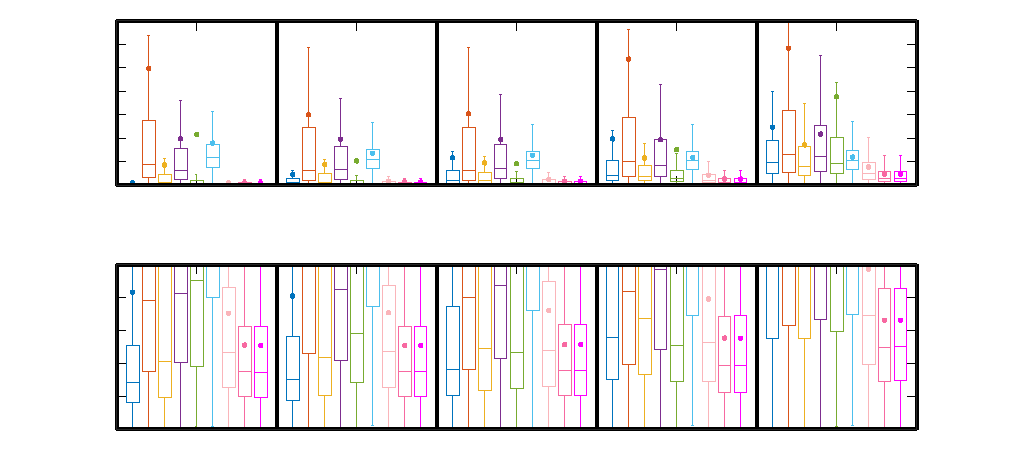
\includegraphics{./figures/parts/02/chapters/04/sections/05/boxplots_pose_errors_sm0}}%
    \gplfronttext
  \end{picture}%
\endgroup

  \end{subfigure}\\\vspace{3cm}%
  \begin{subfigure}{\linewidth}\hspace{-1cm}
    \input{./figures/parts/02/chapters/04/sections/05/boxplots_pose_errors_sm5.tex}
  \end{subfigure}%
  \vspace{1cm}
\caption{\small Οι κατανομές των σφαλμάτων εκτίμησης στάσης για κάθε αλγόριθμο
         με βάση την πειραματική διάταξη της ενότητας
         \ref{subsection:02_04_05:01}. Κάθε ορθογώνιο αντιπροσωπεύει τα
         στατιστικά $\approx 4.5$$\cdot$$10\texttt{e}$$+$$5$ ευθυγραμμίσεων, με
         την εξαίρεση των μεθόδων NDT-PSO και TEASER οι οποίες δοκιμάστηκαν
         $\approx 4.5$$\cdot$$10\texttt{e}$$+$$4$ φορές. Οι κουκίδες
         αντιπροσωπεύουν ολικά μέσα σφάλματα εκτίμησης}
\label{fig:02_04_05:05}
\end{figure}


Τα σχήματα \ref{fig:02_04_05:06}, \ref{fig:02_04_05:07}, \ref{fig:02_04_05:08},
και \ref{fig:02_04_05:09} αναπαριστούν τα μέτρα των τελικών σφαλμάτων στάσης ως
προς τα αρχικά σφάλματα προσανατολισμού (οριζόντιος άξονας) και θέσης
(κάθετος). Συγκεκριμένα, στα πρώτα δύο σχήματα απεικονίζονται τα τελικά
σφάλματα για $\sigma_{\bm{M}} = 0.0$ m $\sigma_{\bm{M}} = 0.05$ αντίστοιχα,
κατακερματισμένα σε ομάδες μέτρων σφάλματος εκτίμησης. Στα δύο τελευταία
σχήματα απεικονίζονται τα ίδια σφάλματα αλλά εστιασμένα ως προς τις ελάχιστες
τιμές, με άνω όριο τον ολικό μέσο όρο σφαλμάτων εκτίμησης στάσης ανά επίπεδο
διαφθοράς χάρτη.


\begin{figure}[!h]\vspace{1cm}\hspace{0.5cm}
  % GNUPLOT: LaTeX picture with Postscript
\begingroup
  \makeatletter
  \providecommand\color[2][]{%
    \GenericError{(gnuplot) \space\space\space\@spaces}{%
      Package color not loaded in conjunction with
      terminal option `colourtext'%
    }{See the gnuplot documentation for explanation.%
    }{Either use 'blacktext' in gnuplot or load the package
      color.sty in LaTeX.}%
    \renewcommand\color[2][]{}%
  }%
  \providecommand\includegraphics[2][]{%
    \GenericError{(gnuplot) \space\space\space\@spaces}{%
      Package graphicx or graphics not loaded%
    }{See the gnuplot documentation for explanation.%
    }{The gnuplot epslatex terminal needs graphicx.sty or graphics.sty.}%
    \renewcommand\includegraphics[2][]{}%
  }%
  \providecommand\rotatebox[2]{#2}%
  \@ifundefined{ifGPcolor}{%
    \newif\ifGPcolor
    \GPcolorfalse
  }{}%
  \@ifundefined{ifGPblacktext}{%
    \newif\ifGPblacktext
    \GPblacktexttrue
  }{}%
  % define a \g@addto@macro without @ in the name:
  \let\gplgaddtomacro\g@addto@macro
  % define empty templates for all commands taking text:
  \gdef\gplfronttext{}%
  \gdef\gplfronttext{}%
  \makeatother
  \ifGPblacktext
    % no textcolor at all
    \def\colorrgb#1{}%
    \def\colorgray#1{}%
  \else
    % gray or color?
    \ifGPcolor
      \def\colorrgb#1{\color[rgb]{#1}}%
      \def\colorgray#1{\color[gray]{#1}}%
      \expandafter\def\csname LTw\endcsname{\color{white}}%
      \expandafter\def\csname LTb\endcsname{\color{black}}%
      \expandafter\def\csname LTa\endcsname{\color{black}}%
      \expandafter\def\csname LT0\endcsname{\color[rgb]{1,0,0}}%
      \expandafter\def\csname LT1\endcsname{\color[rgb]{0,1,0}}%
      \expandafter\def\csname LT2\endcsname{\color[rgb]{0,0,1}}%
      \expandafter\def\csname LT3\endcsname{\color[rgb]{1,0,1}}%
      \expandafter\def\csname LT4\endcsname{\color[rgb]{0,1,1}}%
      \expandafter\def\csname LT5\endcsname{\color[rgb]{1,1,0}}%
      \expandafter\def\csname LT6\endcsname{\color[rgb]{0,0,0}}%
      \expandafter\def\csname LT7\endcsname{\color[rgb]{1,0.3,0}}%
      \expandafter\def\csname LT8\endcsname{\color[rgb]{0.5,0.5,0.5}}%
    \else
      % gray
      \def\colorrgb#1{\color{black}}%
      \def\colorgray#1{\color[gray]{#1}}%
      \expandafter\def\csname LTw\endcsname{\color{white}}%
      \expandafter\def\csname LTb\endcsname{\color{black}}%
      \expandafter\def\csname LTa\endcsname{\color{black}}%
      \expandafter\def\csname LT0\endcsname{\color{black}}%
      \expandafter\def\csname LT1\endcsname{\color{black}}%
      \expandafter\def\csname LT2\endcsname{\color{black}}%
      \expandafter\def\csname LT3\endcsname{\color{black}}%
      \expandafter\def\csname LT4\endcsname{\color{black}}%
      \expandafter\def\csname LT5\endcsname{\color{black}}%
      \expandafter\def\csname LT6\endcsname{\color{black}}%
      \expandafter\def\csname LT7\endcsname{\color{black}}%
      \expandafter\def\csname LT8\endcsname{\color{black}}%
    \fi
  \fi
  \setlength{\unitlength}{0.0500bp}%
  \begin{picture}(8000.00,10000.00)%
    \gplgaddtomacro\gplfronttext{%
      \colorrgb{0.00,0.00,0.00}%
      \put(716,10200){\makebox(0,0){\strut{}\small $\sigma_R = 0.01$}}%
      \colorrgb{0.00,0.00,0.00}%
      \put(2029,10200){\makebox(0,0){\strut{}\small $\sigma_R = 0.03$}}%
      \colorrgb{0.00,0.00,0.00}%
      \put(3343,10200){\makebox(0,0){\strut{}\small $\sigma_R = 0.05$}}%
      \colorrgb{0.00,0.00,0.00}%
      \put(4656,10200){\makebox(0,0){\strut{}\small $\sigma_R = 0.10$}}%
      \colorrgb{0.00,0.00,0.00}%
      \put(5969,10200){\makebox(0,0){\strut{}\small $\sigma_R = 0.20$ [m]}}%
    }%
    \gplgaddtomacro\gplfronttext{%
      \colorrgb{0.00,0.00,0.00}%
      \put(-700,9400){\rotatebox{90}{\makebox(0,0){\strut{}\small PLICP}}}%
      \put(-700,8300){\rotatebox{90}{\makebox(0,0){\strut{}\small NDT}}}%
      \put(-700,7200){\rotatebox{90}{\makebox(0,0){\strut{}\small FastGICP}}}%
      \put(-700,6100){\rotatebox{90}{\makebox(0,0){\strut{}\small FastVGICP}}}%
      \put(-700,5000){\rotatebox{90}{\makebox(0,0){\strut{}\small NDT-PSO}}}%
      \put(-700,3900){\rotatebox{90}{\makebox(0,0){\strut{}\small TEASER}}}%
      \put(-700,2800){\rotatebox{90}{\makebox(0,0){\strut{}\small \texttt{x1}}}}%
      \put(-700,1700){\rotatebox{90}{\makebox(0,0){\strut{}\small \texttt{uf}}}}%
      \put(-700,600){\rotatebox{90}{\makebox(0,0){\strut{}\small \texttt{fm}}}}%
    }%
    \gplgaddtomacro\gplfronttext{%
      \colorrgb{0.00,0.00,0.00}%
      \put(7800,600){\makebox(0,0)[l]{\strut{}$<0.001$}}%
      \colorrgb{0.00,0.00,0.00}%
      \put(7800,1700){\makebox(0,0)[l]{\strut{}$<0.01$}}%
      \colorrgb{0.00,0.00,0.00}%
      \put(7800,2800){\makebox(0,0)[l]{\strut{}$<0.05$}}%
      \colorrgb{0.00,0.00,0.00}%
      \put(7800,3900){\makebox(0,0)[l]{\strut{}$<0.10$}}%
      \colorrgb{0.00,0.00,0.00}%
      \put(7800,5000){\makebox(0,0)[l]{\strut{}$<0.20$}}%
      \colorrgb{0.00,0.00,0.00}%
      \put(7800,6100){\makebox(0,0)[l]{\strut{}$<0.50$}}%
      \colorrgb{0.00,0.00,0.00}%
      \put(7800,7200){\makebox(0,0)[l]{\strut{}$<1.0$}}%
      \colorrgb{0.00,0.00,0.00}%
      \put(7800,8300){\makebox(0,0)[l]{\strut{}$<10.0$}}%
      \colorrgb{0.00,0.00,0.00}%
      \put(7800,9400){\makebox(0,0)[l]{\strut{}$\leq e_{\max}^{\sigma_{\bm{M}}} = 29.29$}}%

      \put(-200,5000) {\rotatebox{90}{\makebox(0,0){\strut{}$\|\Delta \hat{\bm{l}}\|_2 \in [0, \sqrt{2} \cdot \overline{\delta}_{xy}]$}}}%
      \put(3343,-156){\makebox(0,0){\strut{}$\Delta\hat{\theta} \in [-\overline{\delta}_\theta, +\overline{\delta}_\theta]$}}
    }%
    \put(0,0){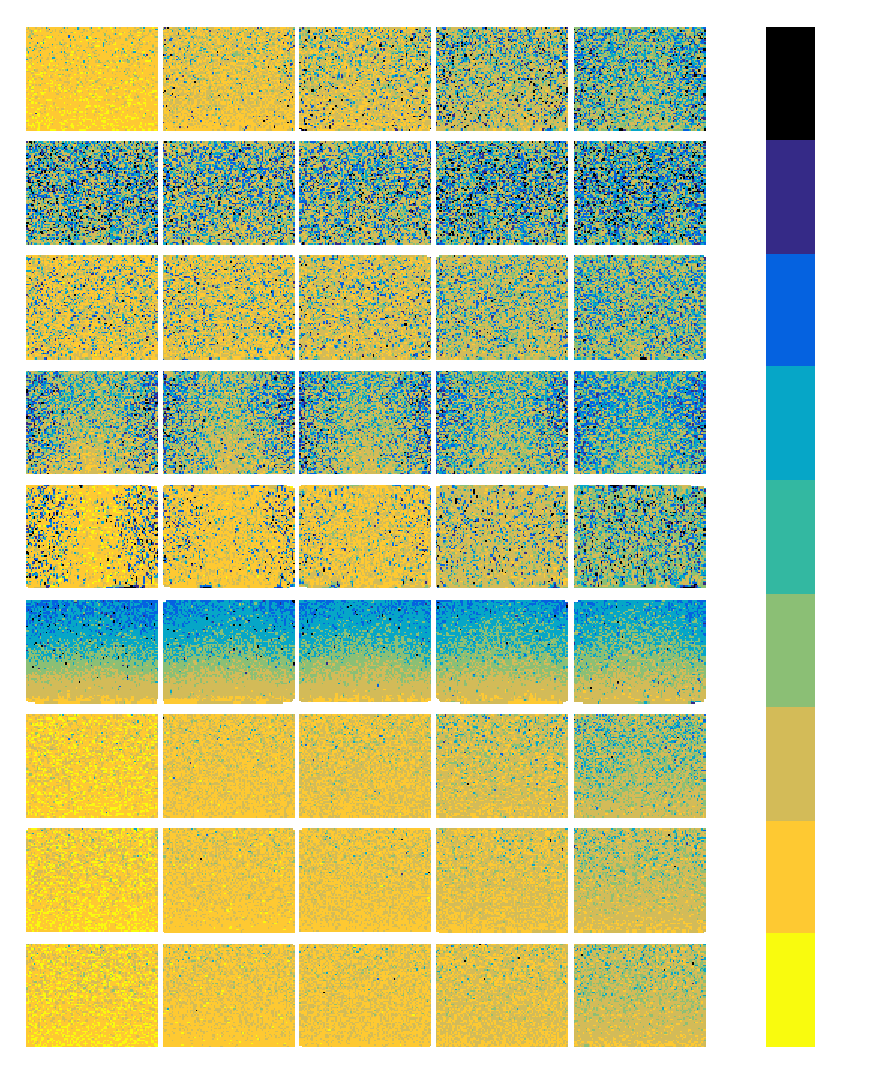
\includegraphics{./figures/parts/02/chapters/04/sections/05/caer_style_pose_errors_binned_sm0}}%
    \gplfronttext
  \end{picture}%
\endgroup

  \vspace{1cm}
  \caption{\small Χάρτες θερμότητας των μέτρων των τελικών σφαλμάτων εκτίμησης
           στάσης συναρτήσει των αρχικών σφαλμάτων εκτίμησης προσανατολισμού
           $\Delta\hat{\theta}$ (στον οριζόντιο άξονα) και των μέτρων των
           αρχικων σφαλμάτων εκτίμησης θέσης $\|\Delta \hat{\bm{l}}\|_2$ (στον
           κάθετο άξονα) για όλα τα διενεργηθέντα πειράματα, ανά αλγόριθμο και
           ανά τυπική απόκλιση διαταραχών του φυσικού αισθητηρα, για
           $\sigma_{\bm{M}} = 0.0$ m}
  \label{fig:02_04_05:06}
\end{figure}

\begin{figure}[!h]\vspace{1cm}\hspace{0.5cm}
  \input{./figures/parts/02/chapters/04/sections/05/caer_style_pose_errors_binned_sm5.tex}
  \vspace{1cm}
  \caption{\small Χάρτες θερμότητας των μέτρων των τελικών σφαλμάτων εκτίμησης
           στάσης συναρτήσει των αρχικών σφαλμάτων εκτίμησης προσανατολισμού
           $\Delta\hat{\theta}$ (στον οριζόντιο άξονα) και των μέτρων των
           αρχικων σφαλμάτων εκτίμησης θέσης $\|\Delta \hat{\bm{l}}\|_2$ (στον
           κάθετο άξονα) για όλα τα διενεργηθέντα πειράματα, ανά αλγόριθμο και
           ανά τυπική απόκλιση διαταραχών του φυσικού αισθητηρα, για
           $\sigma_{\bm{M}} = 0.05$ m}
  \label{fig:02_04_05:07}
\end{figure}

\begin{figure}[!h]\vspace{1cm}\hspace{0.5cm}
  \input{./figures/parts/02/chapters/04/sections/05/caer_style_pose_errors_sm0.tex}
  \vspace{1cm}
  \caption{\small Χάρτες θερμότητας των μέτρων των τελικών σφαλμάτων εκτίμησης
           στάσης συναρτήσει των αρχικών σφαλμάτων εκτίμησης προσανατολισμού
           $\Delta\hat{\theta}$ (στον οριζόντιο άξονα) και των μέτρων των
           αρχικων σφαλμάτων εκτίμησης θέσης $\|\Delta \hat{\bm{l}}\|_2$ (στον
           κάθετο άξονα) για όλα τα διενεργηθέντα πειράματα, ανά αλγόριθμο και
           ανά τυπική απόκλιση διαταραχών του φυσικού αισθητηρα, εστιασμένοι
           στο διάστημα $[0, e_{\sigma_{\bm{M}}}^{\text{avg}}]$, όπου με
           $e_{\sigma_{\bm{M}}}^{\text{avg}}$ σημειώνεται ο μέσος όρος
           σφάλματος εκτίμησης στάσης για κάθε αλγόριθμο, κάθε επεξεργασθέν
           δείγμα, και κάθε τιμή τυπικής απόκλισης των διαταραχών που επιδρούν
           στις μετρήσεις του φυσικού αισθητήρα, για $\sigma_{\bm{M}} = 0.0$ m.
           Τιμές μέτρου σφάλματος εκτίμησης άνω του μέσου όρου σημειώνονται με
           μαύρο χρώμα}
  \label{fig:02_04_05:08}
\end{figure}

\begin{figure}[!h]\vspace{1cm}\hspace{0.5cm}
  \input{./figures/parts/02/chapters/04/sections/05/caer_style_pose_errors_sm5.tex}
  \vspace{1cm}
  \caption{\small Χάρτες θερμότητας των μέτρων των τελικών σφαλμάτων εκτίμησης
           στάσης συναρτήσει των αρχικών σφαλμάτων εκτίμησης προσανατολισμού
           $\Delta\hat{\theta}$ (στον οριζόντιο άξονα) και των μέτρων των
           αρχικων σφαλμάτων εκτίμησης θέσης $\|\Delta \hat{\bm{l}}\|_2$ (στον
           κάθετο άξονα) για όλα τα διενεργηθέντα πειράματα, ανά αλγόριθμο και
           ανά τυπική απόκλιση διαταραχών του φυσικού αισθητηρα, εστιασμένοι
           στο διάστημα $[0, e_{\sigma_{\bm{M}}}^{\text{avg}}]$, όπου με
           $e_{\sigma_{\bm{M}}}^{\text{avg}}$ σημειώνεται ο μέσος όρος
           σφάλματος εκτίμησης στάσης για κάθε αλγόριθμο, κάθε επεξεργασθέν
           δείγμα, και κάθε τιμή τυπικής απόκλισης των διαταραχών που επιδρούν
           στις μετρήσεις του φυσικού αισθητήρα, για $\sigma_{\bm{M}} = 0.05$
           m.  Τιμές μέτρου σφάλματος εκτίμησης άνω του μέσου όρου σημειώνονται
           με μαύρο χρώμα}
  \label{fig:02_04_05:09}
\end{figure}


Τα σχήματα \ref{fig:02_04_05:10}, \ref{fig:02_04_05:11}, και
\ref{fig:02_04_05:12} απεικονίζουν αντίστοιχα τα ποσοστά επίτευξης του στόχου
(\ref{objective:02_04}) ως προς (α) προσανατολισμό ανά μονάδα αρχικού σφάλματος
προσανατολισμού και (β) θέση ανά μονάδα αρχικού σφάλματος εκτίμησης (i) θέσης
και (ii) προσανατολισμού.

\begin{figure}[!h]\centering
  \vspace{2cm}
  \definecolor{c1}{rgb}{0 0.4470 0.7410}
\definecolor{c2}{rgb}{0.8500 0.3250 0.0980}
\definecolor{c3}{rgb}{0.9290 0.6940 0.1250}
\definecolor{c4}{rgb}{0.4940 0.1840 0.5560}
\definecolor{c5}{rgb}{0.4660 0.6740 0.1880}
\definecolor{c6}{rgb}{0.3010 0.7450 0.9330}
\definecolor{c7}{RGB}{251,180,185}
\definecolor{c8}{RGB}{247,104,161}
\definecolor{c9}{RGB}{255,0,255}

% GNUPLOT: LaTeX picture with Postscript
\begingroup
  \makeatletter
  \providecommand\color[2][]{%
    \GenericError{(gnuplot) \space\space\space\@spaces}{%
      Package color not loaded in conjunction with
      terminal option `colourtext'%
    }{See the gnuplot documentation for explanation.%
    }{Either use 'blacktext' in gnuplot or load the package
      color.sty in LaTeX.}%
    \renewcommand\color[2][]{}%
  }%
  \providecommand\includegraphics[2][]{%
    \GenericError{(gnuplot) \space\space\space\@spaces}{%
      Package graphicx or graphics not loaded%
    }{See the gnuplot documentation for explanation.%
    }{The gnuplot epslatex terminal needs graphicx.sty or graphics.sty.}%
    \renewcommand\includegraphics[2][]{}%
  }%
  \providecommand\rotatebox[2]{#2}%
  \@ifundefined{ifGPcolor}{%
    \newif\ifGPcolor
    \GPcolorfalse
  }{}%
  \@ifundefined{ifGPblacktext}{%
    \newif\ifGPblacktext
    \GPblacktexttrue
  }{}%
  % define a \g@addto@macro without @ in the name:
  \let\gplgaddtomacro\g@addto@macro
  % define empty templates for all commands taking text:
  \gdef\gplfronttext{}%
  \gdef\gplfronttext{}%
  \makeatother
  \ifGPblacktext
    % no textcolor at all
    \def\colorrgb#1{}%
    \def\colorgray#1{}%
  \else
    % gray or color?
    \ifGPcolor
      \def\colorrgb#1{\color[rgb]{#1}}%
      \def\colorgray#1{\color[gray]{#1}}%
      \expandafter\def\csname LTw\endcsname{\color{white}}%
      \expandafter\def\csname LTb\endcsname{\color{black}}%
      \expandafter\def\csname LTa\endcsname{\color{black}}%
      \expandafter\def\csname LT0\endcsname{\color[rgb]{1,0,0}}%
      \expandafter\def\csname LT1\endcsname{\color[rgb]{0,1,0}}%
      \expandafter\def\csname LT2\endcsname{\color[rgb]{0,0,1}}%
      \expandafter\def\csname LT3\endcsname{\color[rgb]{1,0,1}}%
      \expandafter\def\csname LT4\endcsname{\color[rgb]{0,1,1}}%
      \expandafter\def\csname LT5\endcsname{\color[rgb]{1,1,0}}%
      \expandafter\def\csname LT6\endcsname{\color[rgb]{0,0,0}}%
      \expandafter\def\csname LT7\endcsname{\color[rgb]{1,0.3,0}}%
      \expandafter\def\csname LT8\endcsname{\color[rgb]{0.5,0.5,0.5}}%
    \else
      % gray
      \def\colorrgb#1{\color{black}}%
      \def\colorgray#1{\color[gray]{#1}}%
      \expandafter\def\csname LTw\endcsname{\color{white}}%
      \expandafter\def\csname LTb\endcsname{\color{black}}%
      \expandafter\def\csname LTa\endcsname{\color{black}}%
      \expandafter\def\csname LT0\endcsname{\color{black}}%
      \expandafter\def\csname LT1\endcsname{\color{black}}%
      \expandafter\def\csname LT2\endcsname{\color{black}}%
      \expandafter\def\csname LT3\endcsname{\color{black}}%
      \expandafter\def\csname LT4\endcsname{\color{black}}%
      \expandafter\def\csname LT5\endcsname{\color{black}}%
      \expandafter\def\csname LT6\endcsname{\color{black}}%
      \expandafter\def\csname LT7\endcsname{\color{black}}%
      \expandafter\def\csname LT8\endcsname{\color{black}}%
    \fi
  \fi
    \setlength{\unitlength}{0.0500bp}%
    \ifx\gptboxheight\undefined%
      \newlength{\gptboxheight}%
      \newlength{\gptboxwidth}%
      \newsavebox{\gptboxtext}%
    \fi%
    \setlength{\fboxrule}{0.5pt}%
    \setlength{\fboxsep}{1pt}%
\begin{picture}(8000.00,4800.00)%
    \gplgaddtomacro\gplfronttext{%
      \colorrgb{0.15,0.15,0.15}%
      \put(-52,2909){\makebox(0,0)[r]{\strut{}\small $80\%$}}%
      \colorrgb{0.15,0.15,0.15}%
      \put(-52,3369){\makebox(0,0)[r]{\strut{}\small $85\%$}}%
      \colorrgb{0.15,0.15,0.15}%
      \put(-52,3830){\makebox(0,0)[r]{\strut{}\small $90\%$}}%
      \colorrgb{0.15,0.15,0.15}%
      \put(-52,4290){\makebox(0,0)[r]{\strut{}\small $95\%$}}%
      \colorrgb{0.15,0.15,0.15}%
      \put(-52,4751){\makebox(0,0)[r]{\strut{}\small $100\%$}}%
      \colorrgb{0.15,0.15,0.15}%
      \put(1583,2228){\makebox(0,0){\strut{}}}%
      \colorrgb{0.15,0.15,0.15}%
      \put(562,2228){\makebox(0,0){\strut{}}}%
      \colorrgb{0.15,0.15,0.15}%
      \put(324,2228){\makebox(0,0){\strut{}}}%
      \colorrgb{0.15,0.15,0.15}%
      \put(86,2228){\makebox(0,0){\strut{}}}%
    }%
    \gplgaddtomacro\gplfronttext{%
      \colorrgb{0.15,0.15,0.15}%
      \put(-718,3599){\rotatebox{90}{\makebox(0,0){\strut{}$\sigma_{\bm{M}} = 0.0$ m}}}%
      \colorrgb{0.00,0.00,0.00}%
      \put(831,4971){\makebox(0,0){\strut{}$\sigma_R = 0.01$ m}}
      \put(3999,5900){\makebox(0,0){\strut{}Ποσοστό επιτυχίας στόχου (\ref{objective:02_04}) ανά μονάδα αρχικής μετατόπισης $|\Delta\theta|$}}%
      \put(0,5400){\makebox(0,0){\strut{}{\color{c1}{\rule[0.6mm]{0.5cm}{0.5mm}}}\small PLICP}}
      \put(1000,5400){\makebox(0,0){\strut{}{\color{c2}{\rule[0.6mm]{0.5cm}{0.5mm}}}\small NDT}}
      \put(2000,5400){\makebox(0,0){\strut{}{\color{c3}{\rule[0.6mm]{0.5cm}{0.5mm}}}\small FastGICP}}
      \put(3400,5400){\makebox(0,0){\strut{}{\color{c4}{\rule[0.6mm]{0.5cm}{0.5mm}}}\small FastVGICP}}
      \put(4800,5400){\makebox(0,0){\strut{}{\color{c5}{\rule[0.6mm]{0.5cm}{0.5mm}}}\small NDT-PSO}}
      \put(6100,5400){\makebox(0,0){\strut{}{\color{c6}{\rule[0.6mm]{0.5cm}{0.5mm}}}\small TEASER}}
      \put(7000,5400){\makebox(0,0){\strut{}{\color{c7}{\rule[0.6mm]{0.5cm}{0.5mm}}}\small x1}}
      \put(7600,5400){\makebox(0,0){\strut{}{\color{c8}{\rule[0.6mm]{0.5cm}{0.5mm}}}\small uf}}
      \put(8200,5400){\makebox(0,0){\strut{}{\color{c9}{\rule[0.6mm]{0.5cm}{0.5mm}}}\small fm}}
      \put(3999,-550){\makebox(0,0){\strut{}Αρχική μετατόπιση $|\Delta \theta|$ [rad]}}%
    }
    \gplgaddtomacro\gplfronttext{
      \colorrgb{0.15,0.15,0.15}
      \put(1532,2448){\makebox(0,0)[r]{\strut{}}}
      \colorrgb{0.15,0.15,0.15}%
      \put(1532,2909){\makebox(0,0)[r]{\strut{}}}%
      \colorrgb{0.15,0.15,0.15}%
      \put(1532,3369){\makebox(0,0)[r]{\strut{}}}%
      \colorrgb{0.15,0.15,0.15}%
      \put(1532,3830){\makebox(0,0)[r]{\strut{}}}%
      \colorrgb{0.15,0.15,0.15}%
      \put(1532,4290){\makebox(0,0)[r]{\strut{}}}%
      \colorrgb{0.15,0.15,0.15}%
      \put(1532,4751){\makebox(0,0)[r]{\strut{}}}%
      \colorrgb{0.15,0.15,0.15}%
      \put(3167,2228){\makebox(0,0){\strut{}}}%
      \colorrgb{0.15,0.15,0.15}%
      \put(2146,2228){\makebox(0,0){\strut{}}}%
      \colorrgb{0.15,0.15,0.15}%
      \put(1908,2228){\makebox(0,0){\strut{}}}%
      \colorrgb{0.15,0.15,0.15}%
      \put(1670,2228){\makebox(0,0){\strut{}}}%
    }%
    \gplgaddtomacro\gplfronttext{%
      \colorrgb{0.00,0.00,0.00}%
      \put(2415,4971){\makebox(0,0){\strut{}$\sigma_R = 0.03$ m}}%
    }%
    \gplgaddtomacro\gplfronttext{%
      \colorrgb{0.15,0.15,0.15}%
      \put(3116,2448){\makebox(0,0)[r]{\strut{}}}%
      \colorrgb{0.15,0.15,0.15}%
      \put(3116,2909){\makebox(0,0)[r]{\strut{}}}%
      \colorrgb{0.15,0.15,0.15}%
      \put(3116,3369){\makebox(0,0)[r]{\strut{}}}%
      \colorrgb{0.15,0.15,0.15}%
      \put(3116,3830){\makebox(0,0)[r]{\strut{}}}%
      \colorrgb{0.15,0.15,0.15}%
      \put(3116,4290){\makebox(0,0)[r]{\strut{}}}%
      \colorrgb{0.15,0.15,0.15}%
      \put(3116,4751){\makebox(0,0)[r]{\strut{}}}%
      \colorrgb{0.15,0.15,0.15}%
      \put(4751,2228){\makebox(0,0){\strut{}}}%
      \colorrgb{0.15,0.15,0.15}%
      \put(3730,2228){\makebox(0,0){\strut{}}}%
      \colorrgb{0.15,0.15,0.15}%
      \put(3492,2228){\makebox(0,0){\strut{}}}%
      \colorrgb{0.15,0.15,0.15}%
      \put(3254,2228){\makebox(0,0){\strut{}}}%
    }%
    \gplgaddtomacro\gplfronttext{%
      \colorrgb{0.00,0.00,0.00}%
      \put(3999,4971){\makebox(0,0){\strut{}$\sigma_R = 0.05$ m}}%
    }%
    \gplgaddtomacro\gplfronttext{%
      \colorrgb{0.15,0.15,0.15}%
      \put(4700,2448){\makebox(0,0)[r]{\strut{}}}%
      \colorrgb{0.15,0.15,0.15}%
      \put(4700,2909){\makebox(0,0)[r]{\strut{}}}%
      \colorrgb{0.15,0.15,0.15}%
      \put(4700,3369){\makebox(0,0)[r]{\strut{}}}%
      \colorrgb{0.15,0.15,0.15}%
      \put(4700,3830){\makebox(0,0)[r]{\strut{}}}%
      \colorrgb{0.15,0.15,0.15}%
      \put(4700,4290){\makebox(0,0)[r]{\strut{}}}%
      \colorrgb{0.15,0.15,0.15}%
      \put(4700,4751){\makebox(0,0)[r]{\strut{}}}%
      \colorrgb{0.15,0.15,0.15}%
      \put(6335,2228){\makebox(0,0){\strut{}}}%
      \colorrgb{0.15,0.15,0.15}%
      \put(5314,2228){\makebox(0,0){\strut{}}}%
      \colorrgb{0.15,0.15,0.15}%
      \put(5076,2228){\makebox(0,0){\strut{}}}%
      \colorrgb{0.15,0.15,0.15}%
      \put(4838,2228){\makebox(0,0){\strut{}}}%
    }%
    \gplgaddtomacro\gplfronttext{%
      \colorrgb{0.00,0.00,0.00}%
      \put(5583,4971){\makebox(0,0){\strut{}$\sigma_R = 0.10$ m}}%
    }%
    \gplgaddtomacro\gplfronttext{%
      \colorrgb{0.15,0.15,0.15}%
      \put(6284,2448){\makebox(0,0)[r]{\strut{}}}%
      \colorrgb{0.15,0.15,0.15}%
      \put(6284,2909){\makebox(0,0)[r]{\strut{}}}%
      \colorrgb{0.15,0.15,0.15}%
      \put(6284,3369){\makebox(0,0)[r]{\strut{}}}%
      \colorrgb{0.15,0.15,0.15}%
      \put(6284,3830){\makebox(0,0)[r]{\strut{}}}%
      \colorrgb{0.15,0.15,0.15}%
      \put(6284,4290){\makebox(0,0)[r]{\strut{}}}%
      \colorrgb{0.15,0.15,0.15}%
      \put(6284,4751){\makebox(0,0)[r]{\strut{}}}%
      \colorrgb{0.15,0.15,0.15}%
      \put(7919,2228){\makebox(0,0){\strut{}}}%
      \colorrgb{0.15,0.15,0.15}%
      \put(6898,2228){\makebox(0,0){\strut{}}}%
      \colorrgb{0.15,0.15,0.15}%
      \put(6660,2228){\makebox(0,0){\strut{}}}%
      \colorrgb{0.15,0.15,0.15}%
      \put(6422,2228){\makebox(0,0){\strut{}}}%
    }%
    \gplgaddtomacro\gplfronttext{%
      \colorrgb{0.00,0.00,0.00}%
      \put(7167,4971){\makebox(0,0){\strut{}$\sigma_R = 0.20$ m}}%
    }%
    \gplgaddtomacro\gplfronttext{%
      \colorrgb{0.15,0.15,0.15}%
      \put(-52,509){\makebox(0,0)[r]{\strut{}\small $80\%$}}%
      \colorrgb{0.15,0.15,0.15}%
      \put(-52,969){\makebox(0,0)[r]{\strut{}\small $85\%$}}%
      \colorrgb{0.15,0.15,0.15}%
      \put(-52,1430){\makebox(0,0)[r]{\strut{}\small $90\%$}}%
      \colorrgb{0.15,0.15,0.15}%
      \put(-52,1890){\makebox(0,0)[r]{\strut{}\small $95\%$}}%
      \colorrgb{0.15,0.15,0.15}%
      \put(-52,2351){\makebox(0,0)[r]{\strut{}\small $100\%$}}%
      \colorrgb{0.15,0.15,0.15}%
      \put(1583,-172){\makebox(0,0){\strut{}\small $\frac{\pi}{4}$}}%
      \colorrgb{0.15,0.15,0.15}%
      \put(562,-172){\makebox(0,0){\strut{}\small $\frac{\pi}{8}$}}%
      \colorrgb{0.15,0.15,0.15}%
      \put(324,-172){\makebox(0,0){\strut{}\small $\frac{\pi}{16}$}}%
      \colorrgb{0.15,0.15,0.15}%
      \put(86,-172){\makebox(0,0){\strut{}\footnotesize $0.0$}}%
    }%
    \gplgaddtomacro\gplfronttext{%
      \colorrgb{0.15,0.15,0.15}%
      \put(-718,1199){\rotatebox{90}{\makebox(0,0){\strut{}$\sigma_{\bm{M}} = 0.05$ m}}}%
    }%
    \gplgaddtomacro\gplfronttext{%
      \colorrgb{0.15,0.15,0.15}%
      \put(1532,48){\makebox(0,0)[r]{\strut{}}}%
      \colorrgb{0.15,0.15,0.15}%
      \put(1532,509){\makebox(0,0)[r]{\strut{}}}%
      \colorrgb{0.15,0.15,0.15}%
      \put(1532,969){\makebox(0,0)[r]{\strut{}}}%
      \colorrgb{0.15,0.15,0.15}%
      \put(1532,1430){\makebox(0,0)[r]{\strut{}}}%
      \colorrgb{0.15,0.15,0.15}%
      \put(1532,1890){\makebox(0,0)[r]{\strut{}}}%
      \colorrgb{0.15,0.15,0.15}%
      \put(1532,2351){\makebox(0,0)[r]{\strut{}}}%
      \colorrgb{0.15,0.15,0.15}%
      \put(3167,-172){\makebox(0,0){\strut{}\small $\frac{\pi}{4}$}}%
      \colorrgb{0.15,0.15,0.15}%
      \put(2146,-172){\makebox(0,0){\strut{}\small $\frac{\pi}{8}$}}%
      \colorrgb{0.15,0.15,0.15}%
      \put(1908,-172){\makebox(0,0){\strut{}\small $\frac{\pi}{16}$}}%
      \colorrgb{0.15,0.15,0.15}%
      %\put(1670,-172){\makebox(0,0){\strut{}\footnotesize $0.0$}}%
    }%
    \gplgaddtomacro\gplfronttext{%
    }%
    \gplgaddtomacro\gplfronttext{%
      \colorrgb{0.15,0.15,0.15}%
      \put(3116,48){\makebox(0,0)[r]{\strut{}}}%
      \colorrgb{0.15,0.15,0.15}%
      \put(3116,509){\makebox(0,0)[r]{\strut{}}}%
      \colorrgb{0.15,0.15,0.15}%
      \put(3116,969){\makebox(0,0)[r]{\strut{}}}%
      \colorrgb{0.15,0.15,0.15}%
      \put(3116,1430){\makebox(0,0)[r]{\strut{}}}%
      \colorrgb{0.15,0.15,0.15}%
      \put(3116,1890){\makebox(0,0)[r]{\strut{}}}%
      \colorrgb{0.15,0.15,0.15}%
      \put(3116,2351){\makebox(0,0)[r]{\strut{}}}%
      \colorrgb{0.15,0.15,0.15}%
      \put(4751,-172){\makebox(0,0){\strut{}\small $\frac{\pi}{4}$}}%
      \colorrgb{0.15,0.15,0.15}%
      \put(3730,-172){\makebox(0,0){\strut{}\small $\frac{\pi}{8}$}}%
      \colorrgb{0.15,0.15,0.15}%
      \put(3492,-172){\makebox(0,0){\strut{}\small $\frac{\pi}{16}$}}%
      \colorrgb{0.15,0.15,0.15}%
      %\put(3254,-172){\makebox(0,0){\strut{}\footnotesize $0.0$}}%
    }%
    \gplgaddtomacro\gplfronttext{%
    }%
    \gplgaddtomacro\gplfronttext{%
      \colorrgb{0.15,0.15,0.15}%
      \put(4700,48){\makebox(0,0)[r]{\strut{}}}%
      \colorrgb{0.15,0.15,0.15}%
      \put(4700,509){\makebox(0,0)[r]{\strut{}}}%
      \colorrgb{0.15,0.15,0.15}%
      \put(4700,969){\makebox(0,0)[r]{\strut{}}}%
      \colorrgb{0.15,0.15,0.15}%
      \put(4700,1430){\makebox(0,0)[r]{\strut{}}}%
      \colorrgb{0.15,0.15,0.15}%
      \put(4700,1890){\makebox(0,0)[r]{\strut{}}}%
      \colorrgb{0.15,0.15,0.15}%
      \put(4700,2351){\makebox(0,0)[r]{\strut{}}}%
      \colorrgb{0.15,0.15,0.15}%
      \put(6335,-172){\makebox(0,0){\strut{}\small $\frac{\pi}{4}$}}%
      \colorrgb{0.15,0.15,0.15}%
      \put(5314,-172){\makebox(0,0){\strut{}\small $\frac{\pi}{8}$}}%
      \colorrgb{0.15,0.15,0.15}%
      \put(5076,-172){\makebox(0,0){\strut{}\small $\frac{\pi}{16}$}}%
      \colorrgb{0.15,0.15,0.15}%
      %\put(4838,-172){\makebox(0,0){\strut{}\footnotesize $0.0$}}%
    }%
    \gplgaddtomacro\gplfronttext{%
    }%
    \gplgaddtomacro\gplfronttext{%
      \colorrgb{0.15,0.15,0.15}%
      \put(6284,48){\makebox(0,0)[r]{\strut{}}}%
      \colorrgb{0.15,0.15,0.15}%
      \put(6284,509){\makebox(0,0)[r]{\strut{}}}%
      \colorrgb{0.15,0.15,0.15}%
      \put(6284,969){\makebox(0,0)[r]{\strut{}}}%
      \colorrgb{0.15,0.15,0.15}%
      \put(6284,1430){\makebox(0,0)[r]{\strut{}}}%
      \colorrgb{0.15,0.15,0.15}%
      \put(6284,1890){\makebox(0,0)[r]{\strut{}}}%
      \colorrgb{0.15,0.15,0.15}%
      \put(6284,2351){\makebox(0,0)[r]{\strut{}}}%
      \colorrgb{0.15,0.15,0.15}%
      \put(7919,-172){\makebox(0,0){\strut{}\small $\frac{\pi}{4}$}}%
      \colorrgb{0.15,0.15,0.15}%
      \put(6898,-172){\makebox(0,0){\strut{}\small $\frac{\pi}{8}$}}%
      \colorrgb{0.15,0.15,0.15}%
      \put(6660,-172){\makebox(0,0){\strut{}\small $\frac{\pi}{16}$}}%
      \colorrgb{0.15,0.15,0.15}%
      %\put(6422,-172){\makebox(0,0){\strut{}\footnotesize $0.0$}}%
    }%
    \gplgaddtomacro\gplfronttext{%
    }%
    \put(0,0){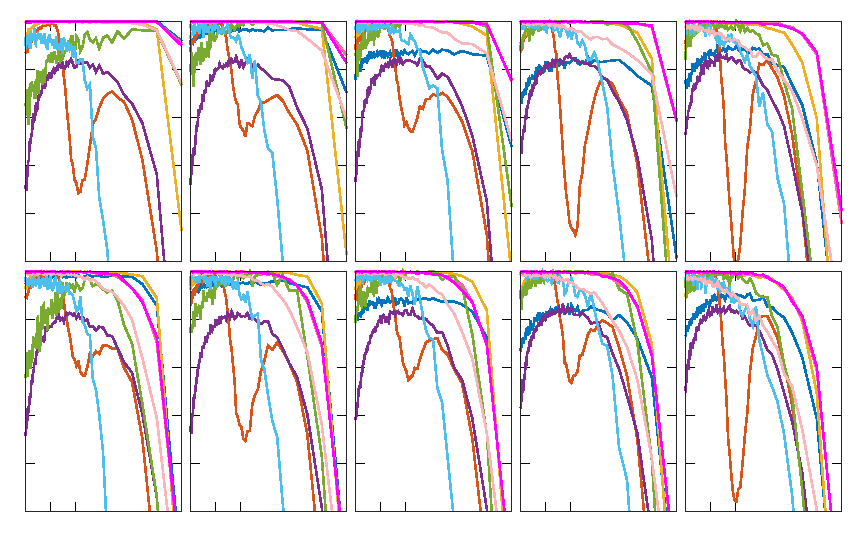
\includegraphics{./figures/parts/02/chapters/04/sections/05/orientation_improvement_percent_binned_curves}}%
    \gplfronttext
  \end{picture}%
\endgroup

  \vspace{1.5cm}
  \caption{\small Οι καμπύλες εξέλιξης των ποσοστών επίτευξης του στόχου
           \ref{objective:02_04} ως προς τη συνιστώσα του προσανατολισμού
           συναρτήσει του μέτρου του αρχικού σφάλματος εκτίμησης
           προσανατολισμού για όλες τις διαμορφώσεις της πειραματικής
           διαδικασίας}
  \label{fig:02_04_05:10}
\end{figure}

\begin{figure}[!h]\centering
  \vspace{2cm}
  \definecolor{c1}{rgb}{0 0.4470 0.7410}
\definecolor{c2}{rgb}{0.8500 0.3250 0.0980}
\definecolor{c3}{rgb}{0.9290 0.6940 0.1250}
\definecolor{c4}{rgb}{0.4940 0.1840 0.5560}
\definecolor{c5}{rgb}{0.4660 0.6740 0.1880}
\definecolor{c6}{rgb}{0.3010 0.7450 0.9330}
\definecolor{c7}{RGB}{251,180,185}
\definecolor{c8}{RGB}{247,104,161}
\definecolor{c9}{RGB}{255,0,255}

% GNUPLOT: LaTeX picture with Postscript
\begingroup
  \makeatletter
  \providecommand\color[2][]{%
    \GenericError{(gnuplot) \space\space\space\@spaces}{%
      Package color not loaded in conjunction with
      terminal option `colourtext'%
    }{See the gnuplot documentation for explanation.%
    }{Either use 'blacktext' in gnuplot or load the package
      color.sty in LaTeX.}%
    \renewcommand\color[2][]{}%
  }%
  \providecommand\includegraphics[2][]{%
    \GenericError{(gnuplot) \space\space\space\@spaces}{%
      Package graphicx or graphics not loaded%
    }{See the gnuplot documentation for explanation.%
    }{The gnuplot epslatex terminal needs graphicx.sty or graphics.sty.}%
    \renewcommand\includegraphics[2][]{}%
  }%
  \providecommand\rotatebox[2]{#2}%
  \@ifundefined{ifGPcolor}{%
    \newif\ifGPcolor
    \GPcolorfalse
  }{}%
  \@ifundefined{ifGPblacktext}{%
    \newif\ifGPblacktext
    \GPblacktexttrue
  }{}%
  % define a \g@addto@macro without @ in the name:
  \let\gplgaddtomacro\g@addto@macro
  % define empty templates for all commands taking text:
  \gdef\gplfronttext{}%
  \gdef\gplfronttext{}%
  \makeatother
  \ifGPblacktext
    % no textcolor at all
    \def\colorrgb#1{}%
    \def\colorgray#1{}%
  \else
    % gray or color?
    \ifGPcolor
      \def\colorrgb#1{\color[rgb]{#1}}%
      \def\colorgray#1{\color[gray]{#1}}%
      \expandafter\def\csname LTw\endcsname{\color{white}}%
      \expandafter\def\csname LTb\endcsname{\color{black}}%
      \expandafter\def\csname LTa\endcsname{\color{black}}%
      \expandafter\def\csname LT0\endcsname{\color[rgb]{1,0,0}}%
      \expandafter\def\csname LT1\endcsname{\color[rgb]{0,1,0}}%
      \expandafter\def\csname LT2\endcsname{\color[rgb]{0,0,1}}%
      \expandafter\def\csname LT3\endcsname{\color[rgb]{1,0,1}}%
      \expandafter\def\csname LT4\endcsname{\color[rgb]{0,1,1}}%
      \expandafter\def\csname LT5\endcsname{\color[rgb]{1,1,0}}%
      \expandafter\def\csname LT6\endcsname{\color[rgb]{0,0,0}}%
      \expandafter\def\csname LT7\endcsname{\color[rgb]{1,0.3,0}}%
      \expandafter\def\csname LT8\endcsname{\color[rgb]{0.5,0.5,0.5}}%
    \else
      % gray
      \def\colorrgb#1{\color{black}}%
      \def\colorgray#1{\color[gray]{#1}}%
      \expandafter\def\csname LTw\endcsname{\color{white}}%
      \expandafter\def\csname LTb\endcsname{\color{black}}%
      \expandafter\def\csname LTa\endcsname{\color{black}}%
      \expandafter\def\csname LT0\endcsname{\color{black}}%
      \expandafter\def\csname LT1\endcsname{\color{black}}%
      \expandafter\def\csname LT2\endcsname{\color{black}}%
      \expandafter\def\csname LT3\endcsname{\color{black}}%
      \expandafter\def\csname LT4\endcsname{\color{black}}%
      \expandafter\def\csname LT5\endcsname{\color{black}}%
      \expandafter\def\csname LT6\endcsname{\color{black}}%
      \expandafter\def\csname LT7\endcsname{\color{black}}%
      \expandafter\def\csname LT8\endcsname{\color{black}}%
    \fi
  \fi
    \setlength{\unitlength}{0.0500bp}%
    \ifx\gptboxheight\undefined%
      \newlength{\gptboxheight}%
      \newlength{\gptboxwidth}%
      \newsavebox{\gptboxtext}%
    \fi%
    \setlength{\fboxrule}{0.5pt}%
    \setlength{\fboxsep}{1pt}%
\begin{picture}(8000.00,4800.00)%
    \gplgaddtomacro\gplfronttext{%
      \colorrgb{0.15,0.15,0.15}%
      %\put(-52,2448){\makebox(0,0)[r]{\strut{}\small $0\%$}}%
      \colorrgb{0.15,0.15,0.15}%
      \put(-52,2909){\makebox(0,0)[r]{\strut{}\small $20\%$}}%
      \colorrgb{0.15,0.15,0.15}%
      \put(-52,3369){\makebox(0,0)[r]{\strut{}\small $40\%$}}%
      \colorrgb{0.15,0.15,0.15}%
      \put(-52,3830){\makebox(0,0)[r]{\strut{}\small $60\%$}}%
      \colorrgb{0.15,0.15,0.15}%
      \put(-52,4290){\makebox(0,0)[r]{\strut{}\small $80\%$}}%
      \colorrgb{0.15,0.15,0.15}%
      \put(-52,4751){\makebox(0,0)[r]{\strut{}\small $100\%$}}%
      \colorrgb{0.15,0.15,0.15}%
      \put(80,2228){\makebox(0,0){\strut{}}}%
      \colorrgb{0.15,0.15,0.15}%
      \put(456,2228){\makebox(0,0){\strut{}}}%
      \colorrgb{0.15,0.15,0.15}%
      \put(832,2228){\makebox(0,0){\strut{}}}%
      \colorrgb{0.15,0.15,0.15}%
      \put(1207,2228){\makebox(0,0){\strut{}}}%
      \colorrgb{0.15,0.15,0.15}%
      \put(1583,2228){\makebox(0,0){\strut{}}}%
    }%
    \gplgaddtomacro\gplfronttext{%
      \colorrgb{0.15,0.15,0.15}%
      \put(-718,3599){\rotatebox{90}{\makebox(0,0){\strut{}$\sigma_{\bm{M}} = 0.0$ m}}}%
      \colorrgb{0.00,0.00,0.00}%
      \put(831,4971){\makebox(0,0){\strut{}$\sigma_R = 0.01$ m}}%

      \put(3999,5900){\makebox(0,0){\strut{}Ποσοστό επιτυχίας στόχου (\ref{objective:02_04}) ως προς θέση ανά μονάδα αρχικής μετατόπισης $(\Delta x^2 + \Delta y^2)^{1/2}$}}%
      \put(0,5400){\makebox(0,0){\strut{}{\color{c1}{\rule[0.6mm]{0.5cm}{0.5mm}}}\small PLICP}}
      \put(1000,5400){\makebox(0,0){\strut{}{\color{c2}{\rule[0.6mm]{0.5cm}{0.5mm}}}\small NDT}}
      \put(2000,5400){\makebox(0,0){\strut{}{\color{c3}{\rule[0.6mm]{0.5cm}{0.5mm}}}\small FastGICP}}
      \put(3400,5400){\makebox(0,0){\strut{}{\color{c4}{\rule[0.6mm]{0.5cm}{0.5mm}}}\small FastVGICP}}
      \put(4800,5400){\makebox(0,0){\strut{}{\color{c5}{\rule[0.6mm]{0.5cm}{0.5mm}}}\small NDT-PSO}}
      \put(6100,5400){\makebox(0,0){\strut{}{\color{c6}{\rule[0.6mm]{0.5cm}{0.5mm}}}\small TEASER}}
      \put(7000,5400){\makebox(0,0){\strut{}{\color{c7}{\rule[0.6mm]{0.5cm}{0.5mm}}}\small \texttt{x1}}}
      \put(7600,5400){\makebox(0,0){\strut{}{\color{c8}{\rule[0.6mm]{0.5cm}{0.5mm}}}\small \texttt{uf}}}
      \put(8200,5400){\makebox(0,0){\strut{}{\color{c9}{\rule[0.6mm]{0.5cm}{0.5mm}}}\small \texttt{fm}}}
      \put(3999,-550){\makebox(0,0){\strut{}Αρχική μετατόπιση $(\Delta x^2 + \Delta y^2)^{1/2}$ [cm]}}%
    }%
    \gplgaddtomacro\gplfronttext{%
      \colorrgb{0.15,0.15,0.15}%
      \put(1532,2448){\makebox(0,0)[r]{\strut{}}}%
      \colorrgb{0.15,0.15,0.15}%
      \put(1532,2909){\makebox(0,0)[r]{\strut{}}}%
      \colorrgb{0.15,0.15,0.15}%
      \put(1532,3369){\makebox(0,0)[r]{\strut{}}}%
      \colorrgb{0.15,0.15,0.15}%
      \put(1532,3830){\makebox(0,0)[r]{\strut{}}}%
      \colorrgb{0.15,0.15,0.15}%
      \put(1532,4290){\makebox(0,0)[r]{\strut{}}}%
      \colorrgb{0.15,0.15,0.15}%
      \put(1532,4751){\makebox(0,0)[r]{\strut{}}}%
      \colorrgb{0.15,0.15,0.15}%
      \put(1664,2228){\makebox(0,0){\strut{}}}%
      \colorrgb{0.15,0.15,0.15}%
      \put(2040,2228){\makebox(0,0){\strut{}}}%
      \colorrgb{0.15,0.15,0.15}%
      \put(2416,2228){\makebox(0,0){\strut{}}}%
      \colorrgb{0.15,0.15,0.15}%
      \put(2791,2228){\makebox(0,0){\strut{}}}%
      \colorrgb{0.15,0.15,0.15}%
      \put(3167,2228){\makebox(0,0){\strut{}}}%
    }%
    \gplgaddtomacro\gplfronttext{%
      \colorrgb{0.00,0.00,0.00}%
      \put(2415,4971){\makebox(0,0){\strut{}$\sigma_R = 0.03$ m}}%
    }%
    \gplgaddtomacro\gplfronttext{%
      \colorrgb{0.15,0.15,0.15}%
      \put(3116,2448){\makebox(0,0)[r]{\strut{}}}%
      \colorrgb{0.15,0.15,0.15}%
      \put(3116,2909){\makebox(0,0)[r]{\strut{}}}%
      \colorrgb{0.15,0.15,0.15}%
      \put(3116,3369){\makebox(0,0)[r]{\strut{}}}%
      \colorrgb{0.15,0.15,0.15}%
      \put(3116,3830){\makebox(0,0)[r]{\strut{}}}%
      \colorrgb{0.15,0.15,0.15}%
      \put(3116,4290){\makebox(0,0)[r]{\strut{}}}%
      \colorrgb{0.15,0.15,0.15}%
      \put(3116,4751){\makebox(0,0)[r]{\strut{}}}%
      \colorrgb{0.15,0.15,0.15}%
      \put(3248,2228){\makebox(0,0){\strut{}}}%
      \colorrgb{0.15,0.15,0.15}%
      \put(3624,2228){\makebox(0,0){\strut{}}}%
      \colorrgb{0.15,0.15,0.15}%
      \put(4000,2228){\makebox(0,0){\strut{}}}%
      \colorrgb{0.15,0.15,0.15}%
      \put(4375,2228){\makebox(0,0){\strut{}}}%
      \colorrgb{0.15,0.15,0.15}%
      \put(4751,2228){\makebox(0,0){\strut{}}}%
    }%
    \gplgaddtomacro\gplfronttext{%
      \colorrgb{0.00,0.00,0.00}%
      \put(3999,4971){\makebox(0,0){\strut{}$\sigma_R = 0.05$ m}}%
    }%
    \gplgaddtomacro\gplfronttext{%
      \colorrgb{0.15,0.15,0.15}%
      \put(4700,2448){\makebox(0,0)[r]{\strut{}}}%
      \colorrgb{0.15,0.15,0.15}%
      \put(4700,2909){\makebox(0,0)[r]{\strut{}}}%
      \colorrgb{0.15,0.15,0.15}%
      \put(4700,3369){\makebox(0,0)[r]{\strut{}}}%
      \colorrgb{0.15,0.15,0.15}%
      \put(4700,3830){\makebox(0,0)[r]{\strut{}}}%
      \colorrgb{0.15,0.15,0.15}%
      \put(4700,4290){\makebox(0,0)[r]{\strut{}}}%
      \colorrgb{0.15,0.15,0.15}%
      \put(4700,4751){\makebox(0,0)[r]{\strut{}}}%
      \colorrgb{0.15,0.15,0.15}%
      \put(4832,2228){\makebox(0,0){\strut{}}}%
      \colorrgb{0.15,0.15,0.15}%
      \put(5208,2228){\makebox(0,0){\strut{}}}%
      \colorrgb{0.15,0.15,0.15}%
      \put(5584,2228){\makebox(0,0){\strut{}}}%
      \colorrgb{0.15,0.15,0.15}%
      \put(5959,2228){\makebox(0,0){\strut{}}}%
      \colorrgb{0.15,0.15,0.15}%
      \put(6335,2228){\makebox(0,0){\strut{}}}%
    }%
    \gplgaddtomacro\gplfronttext{%
      \colorrgb{0.00,0.00,0.00}%
      \put(5583,4971){\makebox(0,0){\strut{}$\sigma_R = 0.10$ m}}%
    }%
    \gplgaddtomacro\gplfronttext{%
      \colorrgb{0.15,0.15,0.15}%
      \put(6284,2448){\makebox(0,0)[r]{\strut{}}}%
      \colorrgb{0.15,0.15,0.15}%
      \put(6284,2909){\makebox(0,0)[r]{\strut{}}}%
      \colorrgb{0.15,0.15,0.15}%
      \put(6284,3369){\makebox(0,0)[r]{\strut{}}}%
      \colorrgb{0.15,0.15,0.15}%
      \put(6284,3830){\makebox(0,0)[r]{\strut{}}}%
      \colorrgb{0.15,0.15,0.15}%
      \put(6284,4290){\makebox(0,0)[r]{\strut{}}}%
      \colorrgb{0.15,0.15,0.15}%
      \put(6284,4751){\makebox(0,0)[r]{\strut{}}}%
      \colorrgb{0.15,0.15,0.15}%
      \put(6416,2228){\makebox(0,0){\strut{}}}%
      \colorrgb{0.15,0.15,0.15}%
      \put(6792,2228){\makebox(0,0){\strut{}}}%
      \colorrgb{0.15,0.15,0.15}%
      \put(7168,2228){\makebox(0,0){\strut{}}}%
      \colorrgb{0.15,0.15,0.15}%
      \put(7543,2228){\makebox(0,0){\strut{}}}%
      \colorrgb{0.15,0.15,0.15}%
      \put(7919,2228){\makebox(0,0){\strut{}}}%
    }%
    \gplgaddtomacro\gplfronttext{%
      \colorrgb{0.00,0.00,0.00}%
      \put(7167,4971){\makebox(0,0){\strut{}$\sigma_R = 0.20$ m}}%
    }%
    \gplgaddtomacro\gplfronttext{%
      \colorrgb{0.15,0.15,0.15}%
      \put(-52,48){\makebox(0,0)[r]{\strut{}\small $0\%$}}%
      \colorrgb{0.15,0.15,0.15}%
      \put(-52,509){\makebox(0,0)[r]{\strut{}\small $20\%$}}%
      \colorrgb{0.15,0.15,0.15}%
      \put(-52,969){\makebox(0,0)[r]{\strut{}\small $40\%$}}%
      \colorrgb{0.15,0.15,0.15}%
      \put(-52,1430){\makebox(0,0)[r]{\strut{}\small $60\%$}}%
      \colorrgb{0.15,0.15,0.15}%
      \put(-52,1890){\makebox(0,0)[r]{\strut{}\small $80\%$}}%
      \colorrgb{0.15,0.15,0.15}%
      \put(-52,2351){\makebox(0,0)[r]{\strut{}\small $100\%$}}%
      \colorrgb{0.15,0.15,0.15}%
      \put(80,-172){\makebox(0,0){\strut{}\footnotesize $0$}}%
      \colorrgb{0.15,0.15,0.15}%
      \put(456,-172){\makebox(0,0){\strut{}\footnotesize $7$}}%
      \colorrgb{0.15,0.15,0.15}%
      \put(832,-172){\makebox(0,0){\strut{}\footnotesize $14$}}%
      \colorrgb{0.15,0.15,0.15}%
      \put(1207,-172){\makebox(0,0){\strut{}\footnotesize $21$}}%
      \colorrgb{0.15,0.15,0.15}%
      \put(1583,-172){\makebox(0,0){\strut{}\footnotesize $28$}}%
    }%
    \gplgaddtomacro\gplfronttext{%
      \colorrgb{0.15,0.15,0.15}%
      \put(-718,1199){\rotatebox{90}{\makebox(0,0){\strut{}$\sigma_{\bm{M}} = 0.05$ m}}}%
    }%
    \gplgaddtomacro\gplfronttext{%
      \colorrgb{0.15,0.15,0.15}%
      \put(1532,48){\makebox(0,0)[r]{\strut{}}}%
      \colorrgb{0.15,0.15,0.15}%
      \put(1532,509){\makebox(0,0)[r]{\strut{}}}%
      \colorrgb{0.15,0.15,0.15}%
      \put(1532,969){\makebox(0,0)[r]{\strut{}}}%
      \colorrgb{0.15,0.15,0.15}%
      \put(1532,1430){\makebox(0,0)[r]{\strut{}}}%
      \colorrgb{0.15,0.15,0.15}%
      \put(1532,1890){\makebox(0,0)[r]{\strut{}}}%
      \colorrgb{0.15,0.15,0.15}%
      \put(1532,2351){\makebox(0,0)[r]{\strut{}}}%
      \colorrgb{0.15,0.15,0.15}%
      %\put(1664,-172){\makebox(0,0){\strut{}\footnotesize $0$}}%
      \colorrgb{0.15,0.15,0.15}%
      \put(2040,-172){\makebox(0,0){\strut{}\footnotesize $7$}}%
      \colorrgb{0.15,0.15,0.15}%
      \put(2416,-172){\makebox(0,0){\strut{}\footnotesize $14$}}%
      \colorrgb{0.15,0.15,0.15}%
      \put(2791,-172){\makebox(0,0){\strut{}\footnotesize $21$}}%
      \colorrgb{0.15,0.15,0.15}%
      \put(3167,-172){\makebox(0,0){\strut{}\footnotesize $28$}}%
    }%
    \gplgaddtomacro\gplfronttext{%
    }%
    \gplgaddtomacro\gplfronttext{%
      \colorrgb{0.15,0.15,0.15}%
      \put(3116,48){\makebox(0,0)[r]{\strut{}}}%
      \colorrgb{0.15,0.15,0.15}%
      \put(3116,509){\makebox(0,0)[r]{\strut{}}}%
      \colorrgb{0.15,0.15,0.15}%
      \put(3116,969){\makebox(0,0)[r]{\strut{}}}%
      \colorrgb{0.15,0.15,0.15}%
      \put(3116,1430){\makebox(0,0)[r]{\strut{}}}%
      \colorrgb{0.15,0.15,0.15}%
      \put(3116,1890){\makebox(0,0)[r]{\strut{}}}%
      \colorrgb{0.15,0.15,0.15}%
      \put(3116,2351){\makebox(0,0)[r]{\strut{}}}%
      \colorrgb{0.15,0.15,0.15}%
      %\put(3248,-172){\makebox(0,0){\strut{}\footnotesize $0$}}%
      \colorrgb{0.15,0.15,0.15}%
      \put(3624,-172){\makebox(0,0){\strut{}\footnotesize $7$}}%
      \colorrgb{0.15,0.15,0.15}%
      \put(4000,-172){\makebox(0,0){\strut{}\footnotesize $14$}}%
      \colorrgb{0.15,0.15,0.15}%
      \put(4375,-172){\makebox(0,0){\strut{}\footnotesize $21$}}%
      \colorrgb{0.15,0.15,0.15}%
      \put(4751,-172){\makebox(0,0){\strut{}\footnotesize $28$}}%
    }%
    \gplgaddtomacro\gplfronttext{%
    }%
    \gplgaddtomacro\gplfronttext{%
      \colorrgb{0.15,0.15,0.15}%
      \put(4700,48){\makebox(0,0)[r]{\strut{}}}%
      \colorrgb{0.15,0.15,0.15}%
      \put(4700,509){\makebox(0,0)[r]{\strut{}}}%
      \colorrgb{0.15,0.15,0.15}%
      \put(4700,969){\makebox(0,0)[r]{\strut{}}}%
      \colorrgb{0.15,0.15,0.15}%
      \put(4700,1430){\makebox(0,0)[r]{\strut{}}}%
      \colorrgb{0.15,0.15,0.15}%
      \put(4700,1890){\makebox(0,0)[r]{\strut{}}}%
      \colorrgb{0.15,0.15,0.15}%
      \put(4700,2351){\makebox(0,0)[r]{\strut{}}}%
      \colorrgb{0.15,0.15,0.15}%
      %\put(4832,-172){\makebox(0,0){\strut{}\footnotesize $0$}}%
      \colorrgb{0.15,0.15,0.15}%
      \put(5208,-172){\makebox(0,0){\strut{}\footnotesize $7$}}%
      \colorrgb{0.15,0.15,0.15}%
      \put(5584,-172){\makebox(0,0){\strut{}\footnotesize $14$}}%
      \colorrgb{0.15,0.15,0.15}%
      \put(5959,-172){\makebox(0,0){\strut{}\footnotesize $21$}}%
      \colorrgb{0.15,0.15,0.15}%
      \put(6335,-172){\makebox(0,0){\strut{}\footnotesize $28$}}%
    }%
    \gplgaddtomacro\gplfronttext{%
    }%
    \gplgaddtomacro\gplfronttext{%
      \colorrgb{0.15,0.15,0.15}%
      \put(6284,48){\makebox(0,0)[r]{\strut{}}}%
      \colorrgb{0.15,0.15,0.15}%
      \put(6284,509){\makebox(0,0)[r]{\strut{}}}%
      \colorrgb{0.15,0.15,0.15}%
      \put(6284,969){\makebox(0,0)[r]{\strut{}}}%
      \colorrgb{0.15,0.15,0.15}%
      \put(6284,1430){\makebox(0,0)[r]{\strut{}}}%
      \colorrgb{0.15,0.15,0.15}%
      \put(6284,1890){\makebox(0,0)[r]{\strut{}}}%
      \colorrgb{0.15,0.15,0.15}%
      \put(6284,2351){\makebox(0,0)[r]{\strut{}}}%
      \colorrgb{0.15,0.15,0.15}%
      %\put(6416,-172){\makebox(0,0){\strut{}\footnotesize $0$}}%
      \colorrgb{0.15,0.15,0.15}%
      \put(6792,-172){\makebox(0,0){\strut{}\footnotesize $7$}}%
      \colorrgb{0.15,0.15,0.15}%
      \put(7168,-172){\makebox(0,0){\strut{}\footnotesize $14$}}%
      \colorrgb{0.15,0.15,0.15}%
      \put(7543,-172){\makebox(0,0){\strut{}\footnotesize $21$}}%
      \colorrgb{0.15,0.15,0.15}%
      \put(7919,-172){\makebox(0,0){\strut{}\footnotesize $28$}}%
    }%
    \gplgaddtomacro\gplfronttext{%
    }%
    \put(0,0){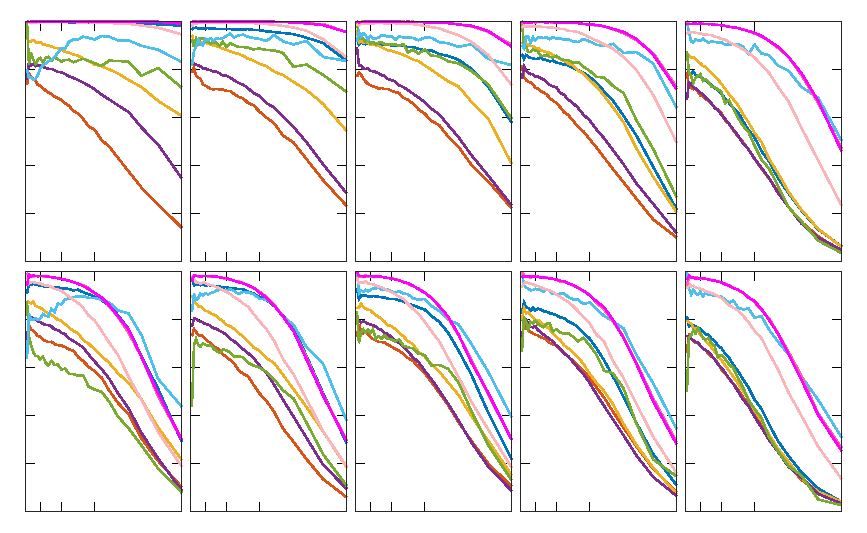
\includegraphics{./figures/parts/02/chapters/04/sections/05/position_improvement_percent_binned_curves}}%
    \gplfronttext
  \end{picture}%
\endgroup

  \vspace{1.5cm}
  \caption{\small Οι καμπύλες εξέλιξης των ποσοστών επίτευξης του στόχου
           \ref{objective:02_04} ως προς τη συνιστώσα της θέσης
           συναρτήσει του μέτρου του αρχικού σφάλματος εκτίμησης
           θέσης για όλες τις διαμορφώσεις της πειραματικής διαδικασίας}
  \label{fig:02_04_05:11}
\end{figure}


\begin{figure}[!h]\centering
  \vspace{2cm}
  \definecolor{c1}{rgb}{0 0.4470 0.7410}
\definecolor{c2}{rgb}{0.8500 0.3250 0.0980}
\definecolor{c3}{rgb}{0.9290 0.6940 0.1250}
\definecolor{c4}{rgb}{0.4940 0.1840 0.5560}
\definecolor{c5}{rgb}{0.4660 0.6740 0.1880}
\definecolor{c6}{rgb}{0.3010 0.7450 0.9330}
\definecolor{c7}{RGB}{251,180,185}
\definecolor{c8}{RGB}{247,104,161}
\definecolor{c9}{RGB}{255,0,255}

% GNUPLOT: LaTeX picture with Postscript
\begingroup
  \makeatletter
  \providecommand\color[2][]{%
    \GenericError{(gnuplot) \space\space\space\@spaces}{%
      Package color not loaded in conjunction with
      terminal option `colourtext'%
    }{See the gnuplot documentation for explanation.%
    }{Either use 'blacktext' in gnuplot or load the package
      color.sty in LaTeX.}%
    \renewcommand\color[2][]{}%
  }%
  \providecommand\includegraphics[2][]{%
    \GenericError{(gnuplot) \space\space\space\@spaces}{%
      Package graphicx or graphics not loaded%
    }{See the gnuplot documentation for explanation.%
    }{The gnuplot epslatex terminal needs graphicx.sty or graphics.sty.}%
    \renewcommand\includegraphics[2][]{}%
  }%
  \providecommand\rotatebox[2]{#2}%
  \@ifundefined{ifGPcolor}{%
    \newif\ifGPcolor
    \GPcolorfalse
  }{}%
  \@ifundefined{ifGPblacktext}{%
    \newif\ifGPblacktext
    \GPblacktexttrue
  }{}%
  % define a \g@addto@macro without @ in the name:
  \let\gplgaddtomacro\g@addto@macro
  % define empty templates for all commands taking text:
  \gdef\gplfronttext{}%
  \gdef\gplfronttext{}%
  \makeatother
  \ifGPblacktext
    % no textcolor at all
    \def\colorrgb#1{}%
    \def\colorgray#1{}%
  \else
    % gray or color?
    \ifGPcolor
      \def\colorrgb#1{\color[rgb]{#1}}%
      \def\colorgray#1{\color[gray]{#1}}%
      \expandafter\def\csname LTw\endcsname{\color{white}}%
      \expandafter\def\csname LTb\endcsname{\color{black}}%
      \expandafter\def\csname LTa\endcsname{\color{black}}%
      \expandafter\def\csname LT0\endcsname{\color[rgb]{1,0,0}}%
      \expandafter\def\csname LT1\endcsname{\color[rgb]{0,1,0}}%
      \expandafter\def\csname LT2\endcsname{\color[rgb]{0,0,1}}%
      \expandafter\def\csname LT3\endcsname{\color[rgb]{1,0,1}}%
      \expandafter\def\csname LT4\endcsname{\color[rgb]{0,1,1}}%
      \expandafter\def\csname LT5\endcsname{\color[rgb]{1,1,0}}%
      \expandafter\def\csname LT6\endcsname{\color[rgb]{0,0,0}}%
      \expandafter\def\csname LT7\endcsname{\color[rgb]{1,0.3,0}}%
      \expandafter\def\csname LT8\endcsname{\color[rgb]{0.5,0.5,0.5}}%
    \else
      % gray
      \def\colorrgb#1{\color{black}}%
      \def\colorgray#1{\color[gray]{#1}}%
      \expandafter\def\csname LTw\endcsname{\color{white}}%
      \expandafter\def\csname LTb\endcsname{\color{black}}%
      \expandafter\def\csname LTa\endcsname{\color{black}}%
      \expandafter\def\csname LT0\endcsname{\color{black}}%
      \expandafter\def\csname LT1\endcsname{\color{black}}%
      \expandafter\def\csname LT2\endcsname{\color{black}}%
      \expandafter\def\csname LT3\endcsname{\color{black}}%
      \expandafter\def\csname LT4\endcsname{\color{black}}%
      \expandafter\def\csname LT5\endcsname{\color{black}}%
      \expandafter\def\csname LT6\endcsname{\color{black}}%
      \expandafter\def\csname LT7\endcsname{\color{black}}%
      \expandafter\def\csname LT8\endcsname{\color{black}}%
    \fi
  \fi
    \setlength{\unitlength}{0.0500bp}%
    \ifx\gptboxheight\undefined%
      \newlength{\gptboxheight}%
      \newlength{\gptboxwidth}%
      \newsavebox{\gptboxtext}%
    \fi%
    \setlength{\fboxrule}{0.5pt}%
    \setlength{\fboxsep}{1pt}%
\begin{picture}(8000.00,4800.00)%
    \gplgaddtomacro\gplfronttext{%
      \colorrgb{0.15,0.15,0.15}%
      %\put(-52,2448){\makebox(0,0)[r]{\strut{}$40\%$}}%
      \colorrgb{0.15,0.15,0.15}%
      \put(-52,3216){\makebox(0,0)[r]{\strut{}$60\%$}}%
      \colorrgb{0.15,0.15,0.15}%
      \put(-52,3983){\makebox(0,0)[r]{\strut{}$80\%$}}%
      \colorrgb{0.15,0.15,0.15}%
      \put(-52,4751){\makebox(0,0)[r]{\strut{}$100\%$}}%
      \colorrgb{0.15,0.15,0.15}%
      \put(80,2228){\makebox(0,0){\strut{}}}%
      \colorrgb{0.15,0.15,0.15}%
      \put(439,2228){\makebox(0,0){\strut{}}}%
      \colorrgb{0.15,0.15,0.15}%
      \put(817,2228){\makebox(0,0){\strut{}}}%
      \colorrgb{0.15,0.15,0.15}%
      \put(1574,2228){\makebox(0,0){\strut{}}}%
    }%
    \gplgaddtomacro\gplfronttext{%
      \colorrgb{0.15,0.15,0.15}%
      \put(-718,3599){\rotatebox{90}{\makebox(0,0){\strut{}$\sigma_{\bm{M}} = 0.0$ m}}}%
      \colorrgb{0.00,0.00,0.00}%
      \put(831,4971){\makebox(0,0){\strut{}$\sigma_R = 0.01$ m}}%
      \put(3999,6200){\makebox(0,0){\strut{}Ποσοστό επιτυχίας στόχου (\ref{objective:02_04})}}%
      \put(3999,5900){\makebox(0,0){\strut{}ως προς θέση ανά μονάδα αρχικού σφάλματος εκτίμησης προσανατολισμού $\Delta\hat{\theta}$}}%
      \put(0,5400){\makebox(0,0){\strut{}{\color{c1}{\rule[0.6mm]{0.5cm}{0.5mm}}}PLICP}}
      \put(1000,5400){\makebox(0,0){\strut{}{\color{c2}{\rule[0.6mm]{0.5cm}{0.5mm}}}NDT}}
      \put(2000,5400){\makebox(0,0){\strut{}{\color{c3}{\rule[0.6mm]{0.5cm}{0.5mm}}}FastGICP}}
      \put(3400,5400){\makebox(0,0){\strut{}{\color{c4}{\rule[0.6mm]{0.5cm}{0.5mm}}}FastVGICP}}
      \put(4800,5400){\makebox(0,0){\strut{}{\color{c5}{\rule[0.6mm]{0.5cm}{0.5mm}}}NDT-PSO}}
      \put(6100,5400){\makebox(0,0){\strut{}{\color{c6}{\rule[0.6mm]{0.5cm}{0.5mm}}}TEASER}}
      \put(7000,5400){\makebox(0,0){\strut{}{\color{c7}{\rule[0.6mm]{0.5cm}{0.5mm}}}\texttt{x1}}}
      \put(7600,5400){\makebox(0,0){\strut{}{\color{c8}{\rule[0.6mm]{0.5cm}{0.5mm}}}\texttt{uf}}}
      \put(8200,5400){\makebox(0,0){\strut{}{\color{c9}{\rule[0.6mm]{0.5cm}{0.5mm}}}\texttt{fm}}}
      \put(3999,-550){\makebox(0,0){\strut{}Αρχικό σφάλμα εκτίμησης προσανατολισμού $|\Delta\hat{\theta}|$ [rad]}}%
    }%
    \gplgaddtomacro\gplfronttext{%
      \colorrgb{0.15,0.15,0.15}%
      \put(1532,2448){\makebox(0,0)[r]{\strut{}}}%
      \colorrgb{0.15,0.15,0.15}%
      \put(1532,3216){\makebox(0,0)[r]{\strut{}}}%
      \colorrgb{0.15,0.15,0.15}%
      \put(1532,3983){\makebox(0,0)[r]{\strut{}}}%
      \colorrgb{0.15,0.15,0.15}%
      \put(1532,4751){\makebox(0,0)[r]{\strut{}}}%
      \colorrgb{0.15,0.15,0.15}%
      \put(1664,2228){\makebox(0,0){\strut{}}}%
      \colorrgb{0.15,0.15,0.15}%
      \put(2023,2228){\makebox(0,0){\strut{}}}%
      \colorrgb{0.15,0.15,0.15}%
      \put(2401,2228){\makebox(0,0){\strut{}}}%
      \colorrgb{0.15,0.15,0.15}%
      \put(3158,2228){\makebox(0,0){\strut{}}}%
    }%
    \gplgaddtomacro\gplfronttext{%
      \colorrgb{0.00,0.00,0.00}%
      \put(2415,4971){\makebox(0,0){\strut{}$\sigma_R = 0.03$ m}}%
    }%
    \gplgaddtomacro\gplfronttext{%
      \colorrgb{0.15,0.15,0.15}%
      \put(3116,2448){\makebox(0,0)[r]{\strut{}}}%
      \colorrgb{0.15,0.15,0.15}%
      \put(3116,3216){\makebox(0,0)[r]{\strut{}}}%
      \colorrgb{0.15,0.15,0.15}%
      \put(3116,3983){\makebox(0,0)[r]{\strut{}}}%
      \colorrgb{0.15,0.15,0.15}%
      \put(3116,4751){\makebox(0,0)[r]{\strut{}}}%
      \colorrgb{0.15,0.15,0.15}%
      \put(3248,2228){\makebox(0,0){\strut{}}}%
      \colorrgb{0.15,0.15,0.15}%
      \put(3607,2228){\makebox(0,0){\strut{}}}%
      \colorrgb{0.15,0.15,0.15}%
      \put(3985,2228){\makebox(0,0){\strut{}}}%
      \colorrgb{0.15,0.15,0.15}%
      \put(4742,2228){\makebox(0,0){\strut{}}}%
    }%
    \gplgaddtomacro\gplfronttext{%
      \colorrgb{0.00,0.00,0.00}%
      \put(3999,4971){\makebox(0,0){\strut{}$\sigma_R = 0.05$ m}}%
    }%
    \gplgaddtomacro\gplfronttext{%
      \colorrgb{0.15,0.15,0.15}%
      \put(4700,2448){\makebox(0,0)[r]{\strut{}}}%
      \colorrgb{0.15,0.15,0.15}%
      \put(4700,3216){\makebox(0,0)[r]{\strut{}}}%
      \colorrgb{0.15,0.15,0.15}%
      \put(4700,3983){\makebox(0,0)[r]{\strut{}}}%
      \colorrgb{0.15,0.15,0.15}%
      \put(4700,4751){\makebox(0,0)[r]{\strut{}}}%
      \colorrgb{0.15,0.15,0.15}%
      \put(4832,2228){\makebox(0,0){\strut{}}}%
      \colorrgb{0.15,0.15,0.15}%
      \put(5191,2228){\makebox(0,0){\strut{}}}%
      \colorrgb{0.15,0.15,0.15}%
      \put(5569,2228){\makebox(0,0){\strut{}}}%
      \colorrgb{0.15,0.15,0.15}%
      \put(6326,2228){\makebox(0,0){\strut{}}}%
    }%
    \gplgaddtomacro\gplfronttext{%
      \colorrgb{0.00,0.00,0.00}%
      \put(5583,4971){\makebox(0,0){\strut{}$\sigma_R = 0.10$ m}}%
    }%
    \gplgaddtomacro\gplfronttext{%
      \colorrgb{0.15,0.15,0.15}%
      \put(6284,2448){\makebox(0,0)[r]{\strut{}}}%
      \colorrgb{0.15,0.15,0.15}%
      \put(6284,3216){\makebox(0,0)[r]{\strut{}}}%
      \colorrgb{0.15,0.15,0.15}%
      \put(6284,3983){\makebox(0,0)[r]{\strut{}}}%
      \colorrgb{0.15,0.15,0.15}%
      \put(6284,4751){\makebox(0,0)[r]{\strut{}}}%
      \colorrgb{0.15,0.15,0.15}%
      \put(6416,2228){\makebox(0,0){\strut{}}}%
      \colorrgb{0.15,0.15,0.15}%
      \put(6775,2228){\makebox(0,0){\strut{}}}%
      \colorrgb{0.15,0.15,0.15}%
      \put(7153,2228){\makebox(0,0){\strut{}}}%
      \colorrgb{0.15,0.15,0.15}%
      \put(7910,2228){\makebox(0,0){\strut{}}}%
    }%
    \gplgaddtomacro\gplfronttext{%
      \colorrgb{0.00,0.00,0.00}%
      \put(7167,4971){\makebox(0,0){\strut{}$\sigma_R = 0.20$ m}}%
    }%
    \gplgaddtomacro\gplfronttext{%
      \colorrgb{0.15,0.15,0.15}%
      \put(-52,48){\makebox(0,0)[r]{\strut{}$40\%$}}%
      \colorrgb{0.15,0.15,0.15}%
      \put(-52,816){\makebox(0,0)[r]{\strut{}$60\%$}}%
      \colorrgb{0.15,0.15,0.15}%
      \put(-52,1583){\makebox(0,0)[r]{\strut{}$80\%$}}%
      \colorrgb{0.15,0.15,0.15}%
      \put(-52,2351){\makebox(0,0)[r]{\strut{}$100\%$}}%
      \colorrgb{0.15,0.15,0.15}%
      \put(80,-172){\makebox(0,0){\strut{}$0.0$}}%
      \colorrgb{0.15,0.15,0.15}%
      \put(439,-172){\makebox(0,0){\strut{}$\frac{\pi}{16}$}}%
      \colorrgb{0.15,0.15,0.15}%
      \put(817,-172){\makebox(0,0){\strut{}$\frac{\pi}{8}$}}%
      \colorrgb{0.15,0.15,0.15}%
      \put(1574,-172){\makebox(0,0){\strut{}$\frac{\pi}{4}$}}%
    }%
    \gplgaddtomacro\gplfronttext{%
      \colorrgb{0.15,0.15,0.15}%
      \put(-718,1199){\rotatebox{90}{\makebox(0,0){\strut{}$\sigma_{\bm{M}} = 0.05$ m}}}%
    }%
    \gplgaddtomacro\gplfronttext{%
      \colorrgb{0.15,0.15,0.15}%
      \put(1532,48){\makebox(0,0)[r]{\strut{}}}%
      \colorrgb{0.15,0.15,0.15}%
      \put(1532,816){\makebox(0,0)[r]{\strut{}}}%
      \colorrgb{0.15,0.15,0.15}%
      \put(1532,1583){\makebox(0,0)[r]{\strut{}}}%
      \colorrgb{0.15,0.15,0.15}%
      \put(1532,2351){\makebox(0,0)[r]{\strut{}}}%
      \colorrgb{0.15,0.15,0.15}%
      %\put(1664,-172){\makebox(0,0){\strut{}$0.0$}}%
      \colorrgb{0.15,0.15,0.15}%
      \put(2023,-172){\makebox(0,0){\strut{}$\frac{\pi}{16}$}}%
      \colorrgb{0.15,0.15,0.15}%
      \put(2401,-172){\makebox(0,0){\strut{}$\frac{\pi}{8}$}}%
      \colorrgb{0.15,0.15,0.15}%
      \put(3158,-172){\makebox(0,0){\strut{}$\frac{\pi}{4}$}}%
    }%
    \gplgaddtomacro\gplfronttext{%
    }%
    \gplgaddtomacro\gplfronttext{%
      \colorrgb{0.15,0.15,0.15}%
      \put(3116,48){\makebox(0,0)[r]{\strut{}}}%
      \colorrgb{0.15,0.15,0.15}%
      \put(3116,816){\makebox(0,0)[r]{\strut{}}}%
      \colorrgb{0.15,0.15,0.15}%
      \put(3116,1583){\makebox(0,0)[r]{\strut{}}}%
      \colorrgb{0.15,0.15,0.15}%
      \put(3116,2351){\makebox(0,0)[r]{\strut{}}}%
      \colorrgb{0.15,0.15,0.15}%
      %\put(3248,-172){\makebox(0,0){\strut{}$0.0$}}%
      \colorrgb{0.15,0.15,0.15}%
      \put(3607,-172){\makebox(0,0){\strut{}$\frac{\pi}{16}$}}%
      \colorrgb{0.15,0.15,0.15}%
      \put(3985,-172){\makebox(0,0){\strut{}$\frac{\pi}{8}$}}%
      \colorrgb{0.15,0.15,0.15}%
      \put(4742,-172){\makebox(0,0){\strut{}$\frac{\pi}{4}$}}%
    }%
    \gplgaddtomacro\gplfronttext{%
    }%
    \gplgaddtomacro\gplfronttext{%
      \colorrgb{0.15,0.15,0.15}%
      \put(4700,48){\makebox(0,0)[r]{\strut{}}}%
      \colorrgb{0.15,0.15,0.15}%
      \put(4700,816){\makebox(0,0)[r]{\strut{}}}%
      \colorrgb{0.15,0.15,0.15}%
      \put(4700,1583){\makebox(0,0)[r]{\strut{}}}%
      \colorrgb{0.15,0.15,0.15}%
      \put(4700,2351){\makebox(0,0)[r]{\strut{}}}%
      \colorrgb{0.15,0.15,0.15}%
      %\put(4832,-172){\makebox(0,0){\strut{}$0.0$}}%
      \colorrgb{0.15,0.15,0.15}%
      \put(5191,-172){\makebox(0,0){\strut{}$\frac{\pi}{16}$}}%
      \colorrgb{0.15,0.15,0.15}%
      \put(5569,-172){\makebox(0,0){\strut{}$\frac{\pi}{8}$}}%
      \colorrgb{0.15,0.15,0.15}%
      \put(6326,-172){\makebox(0,0){\strut{}$\frac{\pi}{4}$}}%
    }%
    \gplgaddtomacro\gplfronttext{%
    }%
    \gplgaddtomacro\gplfronttext{%
      \colorrgb{0.15,0.15,0.15}%
      \put(6284,48){\makebox(0,0)[r]{\strut{}}}%
      \colorrgb{0.15,0.15,0.15}%
      \put(6284,816){\makebox(0,0)[r]{\strut{}}}%
      \colorrgb{0.15,0.15,0.15}%
      \put(6284,1583){\makebox(0,0)[r]{\strut{}}}%
      \colorrgb{0.15,0.15,0.15}%
      \put(6284,2351){\makebox(0,0)[r]{\strut{}}}%
      \colorrgb{0.15,0.15,0.15}%
      %\put(6416,-172){\makebox(0,0){\strut{}$0.0$}}%
      \colorrgb{0.15,0.15,0.15}%
      \put(6775,-172){\makebox(0,0){\strut{}$\frac{\pi}{16}$}}%
      \colorrgb{0.15,0.15,0.15}%
      \put(7153,-172){\makebox(0,0){\strut{}$\frac{\pi}{8}$}}%
      \colorrgb{0.15,0.15,0.15}%
      \put(7910,-172){\makebox(0,0){\strut{}$\frac{\pi}{4}$}}%
    }%
    \gplgaddtomacro\gplfronttext{%
    }%
    \put(0,0){\includegraphics{./figures/parts/02/chapters/04/sections/05/cross_position_improvement_percent_orientation_binned_curves}}%
    \gplfronttext
  \end{picture}%
\endgroup

  \vspace{1.5cm}
  \caption{\small Οι καμπύλες εξέλιξης των ποσοστών επίτευξης του στόχου
           \ref{objective:02_04} ως προς τη συνιστώσα της θέσης συναρτήσει του
           μέτρου του αρχικού σφάλματος εκτίμησης προσανατολισμού για όλες τις
           διαμορφώσεις της πειραματικής διαδικασίας}
  \label{fig:02_04_05:12}
\end{figure}

Το σχήμα \ref{fig:02_04_05:13} απεικονίζει για τις τρεις διαμορφώσεις του FSMSM
και κάθε πειραματική διαμόρφωση τα ποσοστά των τελικών σφαλμάτων εκτίμησης
προσανατολισμού τα οποία έχουν μέτρο μικρότερο από $\gamma / 2^{\nu+1}$, για
$\nu = 0,1,\dots,\nu_{\max} = 5$.

\begin{figure}[!h]\centering
  % GNUPLOT: LaTeX picture with Postscript
\begingroup
  \makeatletter
  \providecommand\color[2][]{%
    \GenericError{(gnuplot) \space\space\space\@spaces}{%
      Package color not loaded in conjunction with
      terminal option `colourtext'%
    }{See the gnuplot documentation for explanation.%
    }{Either use 'blacktext' in gnuplot or load the package
      color.sty in LaTeX.}%
    \renewcommand\color[2][]{}%
  }%
  \providecommand\includegraphics[2][]{%
    \GenericError{(gnuplot) \space\space\space\@spaces}{%
      Package graphicx or graphics not loaded%
    }{See the gnuplot documentation for explanation.%
    }{The gnuplot epslatex terminal needs graphicx.sty or graphics.sty.}%
    \renewcommand\includegraphics[2][]{}%
  }%
  \providecommand\rotatebox[2]{#2}%
  \@ifundefined{ifGPcolor}{%
    \newif\ifGPcolor
    \GPcolorfalse
  }{}%
  \@ifundefined{ifGPblacktext}{%
    \newif\ifGPblacktext
    \GPblacktexttrue
  }{}%
  % define a \g@addto@macro without @ in the name:
  \let\gplgaddtomacro\g@addto@macro
  % define empty templates for all commands taking text:
  \gdef\gplfronttext{}%
  \gdef\gplfronttext{}%
  \makeatother
  \ifGPblacktext
    % no textcolor at all
    \def\colorrgb#1{}%
    \def\colorgray#1{}%
  \else
    % gray or color?
    \ifGPcolor
      \def\colorrgb#1{\color[rgb]{#1}}%
      \def\colorgray#1{\color[gray]{#1}}%
      \expandafter\def\csname LTw\endcsname{\color{white}}%
      \expandafter\def\csname LTb\endcsname{\color{black}}%
      \expandafter\def\csname LTa\endcsname{\color{black}}%
      \expandafter\def\csname LT0\endcsname{\color[rgb]{1,0,0}}%
      \expandafter\def\csname LT1\endcsname{\color[rgb]{0,1,0}}%
      \expandafter\def\csname LT2\endcsname{\color[rgb]{0,0,1}}%
      \expandafter\def\csname LT3\endcsname{\color[rgb]{1,0,1}}%
      \expandafter\def\csname LT4\endcsname{\color[rgb]{0,1,1}}%
      \expandafter\def\csname LT5\endcsname{\color[rgb]{1,1,0}}%
      \expandafter\def\csname LT6\endcsname{\color[rgb]{0,0,0}}%
      \expandafter\def\csname LT7\endcsname{\color[rgb]{1,0.3,0}}%
      \expandafter\def\csname LT8\endcsname{\color[rgb]{0.5,0.5,0.5}}%
    \else
      % gray
      \def\colorrgb#1{\color{black}}%
      \def\colorgray#1{\color[gray]{#1}}%
      \expandafter\def\csname LTw\endcsname{\color{white}}%
      \expandafter\def\csname LTb\endcsname{\color{black}}%
      \expandafter\def\csname LTa\endcsname{\color{black}}%
      \expandafter\def\csname LT0\endcsname{\color{black}}%
      \expandafter\def\csname LT1\endcsname{\color{black}}%
      \expandafter\def\csname LT2\endcsname{\color{black}}%
      \expandafter\def\csname LT3\endcsname{\color{black}}%
      \expandafter\def\csname LT4\endcsname{\color{black}}%
      \expandafter\def\csname LT5\endcsname{\color{black}}%
      \expandafter\def\csname LT6\endcsname{\color{black}}%
      \expandafter\def\csname LT7\endcsname{\color{black}}%
      \expandafter\def\csname LT8\endcsname{\color{black}}%
    \fi
  \fi
    \setlength{\unitlength}{0.0500bp}%
    \ifx\gptboxheight\undefined%
      \newlength{\gptboxheight}%
      \newlength{\gptboxwidth}%
      \newsavebox{\gptboxtext}%
    \fi%
    \setlength{\fboxrule}{0.5pt}%
    \setlength{\fboxsep}{1pt}%
\begin{picture}(6000.00,6000.00)%
    \gplgaddtomacro\gplfronttext{%
    }%
    \gplgaddtomacro\gplfronttext{%
      \colorrgb{0.00,0.00,0.00}%
      \put(929,6159){\makebox(0,0){\strut{}$\Delta_0$}}%
      \colorrgb{0.15,0.15,0.15}%
      \put(174,5783){\makebox(0,0)[r]{\strut{}\scriptsize $0.01$}}%
      \colorrgb{0.15,0.15,0.15}%
      \put(174,5471){\makebox(0,0)[r]{\strut{}\scriptsize $0.03$}}%
      \colorrgb{0.15,0.15,0.15}%
      \put(174,5160){\makebox(0,0)[r]{\strut{}\scriptsize $0.05$}}%
      \colorrgb{0.15,0.15,0.15}%
      \put(174,4848){\makebox(0,0)[r]{\strut{}\scriptsize $0.10$}}%
      \colorrgb{0.15,0.15,0.15}%
      \put(174,4536){\makebox(0,0)[r]{\strut{}\scriptsize $0.20$}}%
    }%
    \gplgaddtomacro\gplfronttext{%
    }%
    \gplgaddtomacro\gplfronttext{%
      \colorrgb{0.00,0.00,0.00}%
      \put(2729,6159){\makebox(0,0){\strut{}$\Delta_1$}}%
    }%
    \gplgaddtomacro\gplfronttext{%
    }%
    \gplgaddtomacro\gplfronttext{%
      \colorrgb{0.00,0.00,0.00}%
      \put(4529,6159){\makebox(0,0){\strut{}$\Delta_2$}}%
    }%
    \gplgaddtomacro\gplfronttext{%
    }%
    \gplgaddtomacro\gplfronttext{%
      \colorrgb{0.00,0.00,0.00}%
      \put(929,3999){\makebox(0,0){\strut{}$\Delta_3$}}%
      \colorrgb{0.15,0.15,0.15}%
      \put(174,3623){\makebox(0,0)[r]{\strut{}\scriptsize $0.01$}}%
      \colorrgb{0.15,0.15,0.15}%
      \put(174,3311){\makebox(0,0)[r]{\strut{}\scriptsize $0.03$}}%
      \colorrgb{0.15,0.15,0.15}%
      \put(174,3000){\makebox(0,0)[r]{\strut{}\scriptsize $0.05$}}%
      \colorrgb{0.15,0.15,0.15}%
      \put(174,2688){\makebox(0,0)[r]{\strut{}\scriptsize $0.10$}}%
      \colorrgb{0.15,0.15,0.15}%
      \put(174,2376){\makebox(0,0)[r]{\strut{}\scriptsize $0.20$}}%
      \colorrgb{0.15,0.15,0.15}%
      \put(462,2000){\makebox(0,0){\strut{}$\frac{\gamma}{2^1}$}}%
      \colorrgb{0.15,0.15,0.15}%
      \put(774,2000){\makebox(0,0){\strut{}$\frac{\gamma}{2^2}$}}%
      \colorrgb{0.15,0.15,0.15}%
      \put(1085,2000){\makebox(0,0){\strut{}$\frac{\gamma}{2^3}$}}%
      \colorrgb{0.15,0.15,0.15}%
      \put(1397,2000){\makebox(0,0){\strut{}$\frac{\gamma}{2^4}$}}%
    }%
    \gplgaddtomacro\gplfronttext{%
    }%
    \gplgaddtomacro\gplfronttext{%
      \colorrgb{0.00,0.00,0.00}%
      \put(2729,3999){\makebox(0,0){\strut{}$\Delta_4$}}%
      \colorrgb{0.15,0.15,0.15}%
      \put(2262,2000){\makebox(0,0){\strut{}$\frac{\gamma}{2^1}$}}%
      \colorrgb{0.15,0.15,0.15}%
      \put(2574,2000){\makebox(0,0){\strut{}$\frac{\gamma}{2^2}$}}%
      \colorrgb{0.15,0.15,0.15}%
      \put(2885,2000){\makebox(0,0){\strut{}$\frac{\gamma}{2^3}$}}%
      \colorrgb{0.15,0.15,0.15}%
      \put(3197,2000){\makebox(0,0){\strut{}$\frac{\gamma}{2^4}$}}%
    }%
    \gplgaddtomacro\gplfronttext{%
    }%
    \gplgaddtomacro\gplfronttext{%
      \colorrgb{0.00,0.00,0.00}%
      \put(4529,3999){\makebox(0,0){\strut{}$\Delta_5$}}%
      \colorrgb{0.15,0.15,0.15}%
      \put(4062,2000){\makebox(0,0){\strut{}$\frac{\gamma}{2^1}$}}%
      \colorrgb{0.15,0.15,0.15}%
      \put(4374,2000){\makebox(0,0){\strut{}$\frac{\gamma}{2^2}$}}%
      \colorrgb{0.15,0.15,0.15}%
      \put(4685,2000){\makebox(0,0){\strut{}$\frac{\gamma}{2^3}$}}%
      \colorrgb{0.15,0.15,0.15}%
      \put(4997,2000){\makebox(0,0){\strut{}$\frac{\gamma}{2^4}$}}%
    }%
    \gplgaddtomacro\gplfronttext{%
    }%
    \gplgaddtomacro\gplfronttext{%
    }%
    \gplgaddtomacro\gplfronttext{%
    }%
    \gplgaddtomacro\gplfronttext{%
      \colorrgb{0.15,0.15,0.15}%
      \put(60,1040){\makebox(0,0){\strut{}$0\%$}}%
      \colorrgb{0.15,0.15,0.15}%
      \put(1128,1040){\makebox(0,0){\strut{}$20\%$}}%
      \colorrgb{0.15,0.15,0.15}%
      \put(2196,1040){\makebox(0,0){\strut{}$40\%$}}%
      \colorrgb{0.15,0.15,0.15}%
      \put(3263,1040){\makebox(0,0){\strut{}$60\%$}}%
      \colorrgb{0.15,0.15,0.15}%
      \put(4331,1040){\makebox(0,0){\strut{}$80\%$}}%
      \colorrgb{0.15,0.15,0.15}%
      \put(5399,1040){\makebox(0,0){\strut{}$100\%$}}%
    }%
    \gplfronttext
    \put(0,0){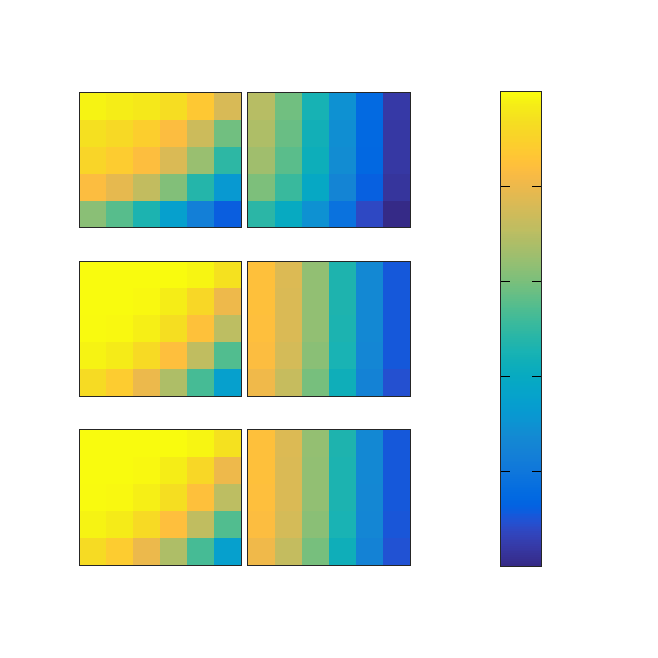
\includegraphics{./figures/parts/02/chapters/05/sections/03/orientation_wrt_gamma}}%
    \gplfronttext
  \end{picture}%
\endgroup

  \vspace{-0.5cm}
  \caption{\small Ποσοστά τελικών σφαλμάτων εκτίμησης προσανατολισμού των
           τριών διαμορφώσεων του FSMSM με μέτρο μικρότερο από $\gamma /
           2^{\nu+1}$, για $\nu = 0,1,\dots,\nu_{\max} = 5$, για όλες τις
           διαμορφώσεις τις πειραματικής διαδικασίας}
  \label{fig:02_04_05:13}
\end{figure}




%%%%%%%%%%%%%%%%%%%%%%%%%%%%%%%%%%%%%%%%%%%%%%%%%%%%%%%%%%%%%%%%%%%%%%%%%%%%%%%%
\subsection{Εξέταση και αξιολόγηση αποτελεσμάτων}
\label{subsection:02_04_05:03}

Με βάση τα πειραματικά αποτελέσματα που εκτίθενται στα σχήματα
\ref{fig:02_04_05:01}-\ref{fig:02_04_05:13} της ενότητας
\ref{subsection:02_04_05:02}, δεδομένης της πειραματικής διάταξης της ενότητας
\ref{subsection:02_04_05:01}, συνάγουμε πρώτα τα πιο βασικά συμπεράσματα:

\begin{framed}
\begin{itemize}
  \item Ο στόχος (\ref{objective:02_04}) επιτυγχάνεται για τον \texttt{x1} σε
        ποσοστό άνω του $97.5\%$ για όλα τα επίπεδα των υπό εξέταση διαταραχών
        $\sigma_R$ και $\sigma_{\bm{M}}$, και για τους \texttt{uf} και
        \texttt{fm} σε ποσοστό άνω του $99.2\%$ (σχήμα \ref{fig:02_04_05:01})
  \item Οι τρεις άνωθεν μέθοδοι εκτελούνται σε πραγματικό χρόνο για αριθμό
        ακτίνων $N_s = 360$, αλλά ο \texttt{x1} υπολείπεται σε χρόνο εκτέλεσης
        σε χαμηλά επίπεδα διαταραχών των μετρήσεων του φυσικού αισθητήρα lidar
        (σχήμα \ref{fig:02_04_05:03})
  \item Τo μέσo σφάλμα εκτίμησης στάσης των \texttt{x1}, \texttt{uf}, και
        \texttt{fm} έχει για άνω όριο τo ελάχιστo μέσο σφάλμα της καλύτερης
        ανά διαμόρφωση μεθοδου (σχήμα \ref{fig:02_04_05:05})
  \item Οι μέθοδοι \texttt{uf} και \texttt{fm} είναι πρακτικά ισοδύναμες ως προς
        όλες τις μετρικές αξιολόγησης (ποσοστό επιτυχίας, σφάλματα εκτίμησης
        θέσης και προσανατολισμού, αριθμό επανεκκινήσεων, χρόνο εκτέλεσης)
\end{itemize}
\end{framed}

Ξεκινώντας από το σχήμα \ref{fig:02_04_05:01}, με βάση τα πειραματικά στοιχεία
παρατηρούμε πως οι μέθο
